\chapter{肝脏}

\section{检查方法}

\subsection{平扫和增强扫描的应用价值}

1.检查前准备:空腹口服1%~2%的泛影葡胺水溶液或白开水500~800ml,上床前再口服200ml。增强扫描者需做碘过敏试验和选择静脉用造影剂。

2.平扫的作用:应作为常规,即使增强者,如无近期平扫片,亦应在注射造影剂前行常规平扫。平扫对造成肝脏密度改变的弥漫性病变如脂肪肝、血管性病变、糖原贮积病、淀粉样变性、Wilson病、血色素沉着以及肝硬化等有重要价值;对肝内钙化灶的显示如肝内胆管结石、血吸虫病肝内钙化、肿瘤钙化等平扫是不可缺少的。平扫应从膈顶开始至肝下端为止。层厚和间隔常规为10mm。对小病灶宜改用薄层(2~5mm)。

3.增强扫描的作用:①进一步发现病变,提高病变的检出率;②根据增强特点有利于确定病变性质;③可鉴别平扫图像上的血管断面、扩张的肝内胆管断面及小结节病变;④可进一步显示肝静脉、门静脉及胆管等结构。

\subsection{造影剂在肝脏内动态循环过程的分期}

下述3期是人为划分的。

1.动脉期:又称为注射期。约在开始注射造影剂后的30秒左右。腹主动脉及其主要分支增强十分显著,CT值>150~200Hu;门静脉和腔静脉尚未显影或密度低于主动脉,肝实质的CT值逐渐上升。早期肝实质的密度偶可不均。

2.门静脉期:又称为非平衡期。持续约60~90秒,造影剂已逐步由血管内向血管外分布,主动脉与腔静脉的密度趋向一致。在静脉早期肝实质的增强达到峰值,以后缓慢下降。

3.平衡期:亦称为延迟期。造影剂在血管内外的分布处于均衡状态,肝内血管影消失。在时间-密度曲线上,主动脉曲线与肝实质曲线开始平行,并以等同速度下降。

\subsection{肝增强扫描常用的方式}

1.团注法增强扫描:以2~3ml/s流率,团注造影剂80~100ml。如扫描范围大时,可采用此法与滴注法相结合。即以2~3ml/s的流率注完50ml后,再改为1ml/s静滴法,将全部造影剂滴完。这样可保持整个扫描过程中,血液中有较高的造影剂浓度。

2.团注动态扫描:适用于扫描速度较慢CT机,可行上述3期扫描。①同层动态扫描:即在平扫或常规扫描发现病变的基础上,确定扫描层面。然后,在同一层面连续增强扫描,每3~5次扫描为1组,该时间内病人屏气;一般行两组扫描,两组间停顿10秒。如疑为血管瘤再行延迟扫描。②进床式动态扫描:以发现病灶为主要目的,扫描范围包括整个肝脏。允许床面移动,每3~5层为1组,该时间内病人屏气,两组之间间隔10秒,让病人呼吸。完成全肝扫描需3~4组。然后进行图像重建、显示和处理。

3.螺旋CT增强扫描:以3ml/s的流率,注入60%造影剂80~100ml。于开始注射造影剂计时,延迟至20~25秒行动脉期,60~90秒行门静脉期,3~4分钟行平衡期扫描。肝动脉期有利于血供丰富性肿瘤的诊断,门静脉期有利于乏血性肿瘤的诊断。

\subsection{肝脏延迟扫描}

它指的是在一次大量注射造影剂后4~6h的重复扫描,与鉴别肝癌与血管瘤的7~15min的延迟扫描含义不同。目的是提高肝内小病灶的检出率。

其原理为泛影葡胺、优维显等有机碘溶液经静脉内注射后大部分经尿路排泄,小部分(10%左右)经肝脏排泄。由于正常肝细胞具有排泄和再吸收有机碘的功能,数小时后肝脏CT衰减值略有提高(CT值升高6~10Hu);而肝癌细胞不具有这种功能,这样两者的密度差异增大,有利于肝癌病灶的检出。但造影剂用量必须足够大,用60%的造影剂150~180ml(结合碘含量50~60g),如增强扫描时注射量不足,待扫描结束后补充注射达上述总剂量。

\subsection{肝动脉造影CT(CTA)}

1.方法:经股动脉插管后(Seldinger法),将导管置于肝动脉内,根据检查目的的不同,可采用同层或进床式动态扫描。经导管注入造影剂,浓度为30%,注射流率1~2ml/s,每次(组)10~20ml。于注射开始后即开始扫描,每3~4层为1组。

如用螺旋CT可行全肝CT检查,对发现多发小病灶更为有利。

2.诊断价值:因肝细胞癌由肝动脉供血,故CTA图像上呈特异性的高密度。此法对诊断小肝癌有一定价值,但有一定假阳性率。此外,对乏血性肿瘤不易检出。

\subsection{肝脏经动脉门静脉造影CT(CTAP)}

1.方法:同样经股动脉插管,将导管置于肠系膜上动脉或脾动脉内。经导管注入造影剂,浓度为60%,注射流率为2~3ml/s。注射开始后20~25秒开始扫描,扫描方法同CTA。

2.诊断价值:CTAP是依据绝大部分肿瘤,尤其是肝细胞癌不接受门脉供血,而正常肝组织血供80%~85%来源于门脉。因而CTAP可明显提高正常肝组织的CT值,而肿瘤组织的CT值无改变或改变甚微,从而提高病变的检出率。此外,亦可有假阳性表现。

\subsection{肝脏碘化油CT}

1.方法:经股动脉插管后,将导管置于肝动脉内,并尽量选择到供血动脉的末梢支,注入5ml碘化油,于7~14天后行CT检查。

2.诊断价值:碘化油能长期选择性地聚集在肝癌组织中。其原因可能与肝癌组织血供丰富、血流量大、血管形态结构异常,癌组织缺乏完整的单核吞噬细胞系统和淋巴系统,以及碘化油颗粒黏度大,难以清除有关。因碘化油能选择性地沉积在肝癌组织内,碘化油CT对小肝癌尤其≤1.5cm病灶的定位、定性有较高的特异性。部分血供丰富的转移瘤亦可有碘化油停滞。一些早期肝细胞癌因肿瘤血管尚不成熟且不丰富,可几乎无碘化油沉积。

\subsection{螺旋CT门静脉成像}

1.检查前准备:主要包括呼吸训练和口服胃肠对比剂,应口服阴性对比剂如水或产气粉为好。

2.扫描参数:①单层螺旋CT:层厚3~5mm不等,螺距1~2,重建间隔1.5~2.5mm。②多层螺旋CT:层厚0.5~1mm用于高分辨率扫描(HQ);层厚5~10mm用于快速扫描(HS)。HQ螺距为3,HS螺距为4.5~6即可。

3.对比剂注射:以3ml/s流率注入60%对比剂100~140ml(约2ml/kg体重)。

4.延迟时间:指开始注射对比剂后至开始扫描的时间间隔,多用50~70秒。

5.重建方式:MIP、MPR、MPVR(多轴向投照容积重建)。

\subsection{肝脏CT灌注成像}

\subsubsection{检查方法}

患者平卧,常规行全肝平扫。层厚及层距10mm或8mm,螺距为1~1.5,扫描速度最少1层/秒。然后选定靶层面,通常包括肝门层面,也可为病灶中心层面;经肘静脉快速团注对比剂,流率为2.5~10ml/s,多为4~5ml/s,用量40~50ml。在对比剂首过前、首过时及其后,按一定时间设置、行同层动态扫描。文献中扫描程序并不相同,Miles等常扫描10次:常规扫描后,于注药后0,7,10,13,16,21,26,31,37.5,44秒各扫描一次,共计10次;其他常用的扫描设置为19~25次。由于4层螺旋CT的广泛应用,采用程序一般为:层厚5mm,间隔为3秒,平静呼吸下行120层扫描。

\subsubsection{图像处理}

先选择兴趣区(ROI),于左右叶肝实质或病灶、脾脏实质、门静脉、主动脉各选一个,在没有包括脾脏者可用肾实质代替。ROI应尽量大,但不能达脏器边缘,以免部分容积效应的影响;实质区ROI尽量不包括大血管。测量该层面不同时间获得的ROI的CT值,可获取其时间-密度曲线(TDC)。接着用灌注软件处理、得出灌注值;如无此软件,则可根据相应公式(下述)计算。

\subsubsection{组织灌流量的计算公式}

组织灌注量(ml·min\textsuperscript{-1} ·ml\textsuperscript{-1}
)=组织TDC的最大斜率(Hu/min)/供血动脉TDC的峰值(Hu)。

\subsubsection{肝灌注成像的灌注参数}

1.肝动脉灌注量(HAP)=脾峰值增强前的肝TDC最大斜率/最大主动脉CT增加值。

2.门静脉灌注量(HPP)=脾峰值增强后的肝TDC最大斜率/最大主动脉CT增加值。但该方法在计算HPP(或PVP)时,未考虑到肝血流中动脉血流的影响,并且以主动脉作为门静脉肝的供血血管进行计算,所得的HPP偏低。国外有学者对此公式进行了改进:HPP=脾峰值增强后的门静脉灌注TDC最大斜率/最大门静脉CT增加值,算得的HPP为0.93,更接近于生理值。

3.肝动脉灌注指数(HPI):为肝动脉灌注占全肝总灌注值(TLP,为HAP和HPP之和)的比例。HPI=HAP/(HAP+HPP)。

4.门静脉灌注指数(PPI):为门静脉灌注占全肝总灌注值的比例。PPI=HPP/(HAP+HPP)。

文献报道的各项正常灌注指标并不一致,如HAP为0.102±0.014、0.091±0.067、0.16、0.19不等;HPP则为1.03±0.43、1.11±0.23、1.22、0.93不等。差异可能为所选病例不同或CT值测量具有误差所致。但总的看来,HAP:HPP≈1∶(3~4)。

近期国内有报道HAP为0.2828±0.0969,HPP为1.1788±0.4004,总肝灌注量为1.4563±0.4439,HPI为(19.71±5.81)%。

\subsubsection{临床应用价值}

①肝硬化:HPP、TLP、PPI明显降低,HAP虽有升高,但无统计学意义。HPP、PPI降低可能是由于肝内组织的阻力增加所致,但HPP降低并不一定出现HAP代偿性升高。②弥漫性肝癌:HPP明显降低,而HAP变化变大,原因同上。③转移性肝癌:转移灶内HAP及邻近肝组织HAP均明显升高。病灶内HAP升高与微血管密度升高一致;邻近组织HAP升高意味着新生血管化,可能是恶性的;HPP多与正常接近,但范围变化大,可异常高或异常低。④肝癌经动脉栓塞治疗(TAE)后:TAE后2~6天HAP明显升高,1个月后降低;而HPP在TAE后2~6天明显降低,1个月后变化不显著。HAP增加可能是栓塞后急性反应所致;而HPP降低可能是因为肝组织内压力增加。⑤肝移植:HAP、HPI增加,而HPP、TLP无统计学差异。HAP增加可能是肝移植后的反应有关。

\section{正常解剖、变异和血管畸形}

\subsection{肝脏表面的解剖结构}

肝脏为人体最大的腺体,分为上下两面。

1.上面:为凸面称为膈面。由镰状韧带从矢状位将肝分为左右两部分,但镰状韧带并非左右两叶的分界标志。

2.下面:为凹面称为脏面。有两条纵沟和一条横沟通过,呈“H”形。左纵沟内有肝圆韧带和静脉韧带;右纵沟的前部为胆囊,后部为下腔静脉。横沟即肝门,内有门静脉、肝动脉和肝管等结构出入肝脏。

\subsection{叶和段的划分}

肝脏被叶间裂和段裂分成若干叶和段。

\subsubsection{肝脏的裂隙}

1.主叶间裂:即正中裂或Cantlie线。基本呈矢状位,将肝脏分成左右两叶。在脏面,该裂相当于胆囊窝中点到下腔静脉左缘的连线,中肝静脉的主干位于该裂隙内。

2.左叶间裂:即脐裂。呈矢状位,将肝左叶分成内侧段(亦称为左内叶,相当于原来的方叶)和外侧段(亦称为左外叶,相当于原来的左叶)。该裂即圆韧带裂隙和静脉韧带裂,在脏面与左纵沟一致。在裂的上部有左肝静脉干(汇入下腔静脉前的一段)通过。但国内刘树伟等认为,该裂断层中为下腔静脉左前缘与肝门静脉左支矢状部的连线,于人体正中矢状轴偏右10°引虚线即为左叶间裂。

尾叶相当于肝脏后部一个突出的部分,以下腔静脉窝为后界,静脉韧带裂隙为前界。尾叶与右叶之间由峡部相连,有时尾叶呈舌状突起自内伸入到门静脉和下腔静脉之间,称为尾叶突。来自左叶和右叶的肝动脉和门静脉分支同时供应尾叶,尾叶的静脉血直接回流到下腔静脉。其血供特点和自成体系的解剖结构,使该部很少患某些弥漫性病变,如肝硬化病人右叶往往萎缩,而尾叶却代偿性增大。

3.背裂:位于尾叶前方,上起第二肝门的下缘,下至第一肝门的后缘。在横断面上,其上部为肝中静脉近侧端的后缘,中部相当于从下腔静脉右前缘至静脉韧带裂右端的弧形线,下部为肝门横沟或肝门静脉的后缘。背裂分隔尾状叶与前方的左内叶、右前叶以及右侧的右后叶。

4.右叶间裂:即右门裂。基本呈冠状位,把右叶分成前段(右前叶)和后段(右后叶)。该裂在肝表面难以确定,内有右肝静脉通过。横断面肝门以上相当于下腔静脉右缘与肝右静脉长轴的连线;肝门以下相当于肝门横沟后缘(或肝门静脉右支)与肝右静脉或其右前、后支之间的连线。

5.左段间裂:即左门裂。呈由后上斜向前下的冠状位。在断层中相当于肝左静脉向外延伸的长轴,将肝左外叶分为上、下两段。但亦有文献在横断面上,以门静脉左支的水平切面为界,将左外叶分为上、下两段。

6.右段间裂:即横裂。断层中,此裂内无肝静脉走行,但通常将门静脉右支或肝门右切迹作为右段间裂的标志,即该平面以上为右半肝的前上或后上段,平面以下为前下或后下段。

\subsubsection{叶和段的划分}

根据以上裂隙可将肝脏分成3叶,即左叶、右叶、尾叶。每叶又分成段和亚段即右叶前段(上段+下段)和后段(上段+下段),左叶的内侧段和外侧段(上段+下段)和尾叶。也有学者将其归结为5叶8段(后述),但其含义是完全一致的。

\subsection{肝脏的功能解剖分段}

目前,对1954年由Couinaud创立的肝脏8段法功能解剖,已得到广泛应用。它是以Glisson系统在肝内的分布为基础,以肝静脉为分段界限。

\subsubsection{Glisson系统}

亦称门管系统,即门静脉、肝动脉、胆管在肝内的分属支相伴而行,被结缔组织纤维鞘包绕而形成的三联管道系统,似树枝状分布于肝内。肝的各段均有Glisson系统的一个分支供血,并引流胆汁,而位于各段之间的肝静脉则引流相邻肝段的回血。因此,每一个段可视为肝的功能解剖单位。

\subsubsection{肝脏分段}

右、中、左3支主肝静脉走行区所形成的纵行切面将肝分割成4个部分,称为4个扇区。由右向左分别称为右后、右前、左内、左外4个扇区。每个扇区又被门脉左、右支的水平切面分成上下两段(见上述:左外叶以左肝静脉向外延伸的长轴、近冠状切面分段可能更趋合理)。4各扇区不包括尾状叶。Ⅰ段:尾状叶,为一个自主段;Ⅱ段:左外扇区(相当于传统的左叶外段)的上部;Ⅲ段:左外扇区的下部;Ⅳ段:左内扇区(相当于传统的左叶内段),在外科临床上还可分为上部的Ⅳa、下部的Ⅳb亚段;Ⅴ段:右前扇区下部;Ⅵ段:右后扇区下部;Ⅶ段:右后扇区上部;Ⅷ段:右前扇区上部。国内刘树伟等将其总结为5叶8段(见表\ref{tab11-1})。

\begin{table}[htbp]
\centering
\caption{Couinaud肝段}
\label{tab11-1}
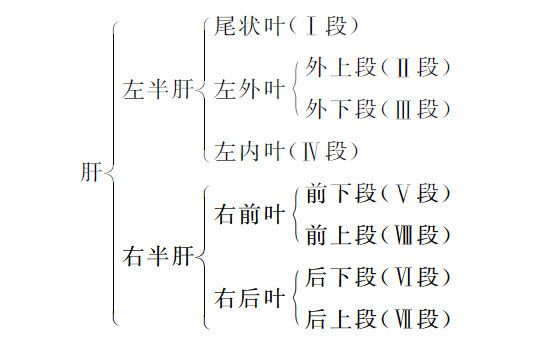
\includegraphics[width=\textwidth,height=\textheight,keepaspectratio]{./images/Image00270.jpg}
\end{table}

在CT检查时,可在下述4个层面上识别肝静脉和门静脉并区分各段:①最头端层面,为3支主肝静脉和下腔静脉汇合的层面;②门静脉左支层面;③门静脉右支层面;④最尾端层面,为门静脉主干和胆囊水平的层面。

\subsection{第二肝门的解剖结构}

1.第一肝门:门管系统经第一肝门(或称肝门)出入肝脏。由门静脉、肝动脉和胆管所构成。门静脉最粗,位于肝动脉和胆管的后方,肝动脉在左,胆管在右。

2.第二肝门:位于肝顶部,为肝左、肝中、肝右静脉汇入下腔静脉处。

\subsection{肝静脉和肝淋巴管的走行}

1.门静脉及其分支:门静脉由脾静脉和肠系膜上静脉汇合而成,门静脉通过肝十二指肠韧带上升到达肝门而分为左、右侧门静脉。门静脉左支供应尾状叶左侧及肝左叶各亚段;门静脉右支供应尾状叶右侧及肝右叶各亚段。在横断面图像上,右侧门静脉较短向下、向右、向后行走,其前后侧分支通常在同一层面。在该层面或向头侧可见到左侧门静脉,该支较长,向前、向左上水平行走一段称为横部(长约22mm,粗约9.4mm),其末端以90°~120°角向前转为矢状部(长约21mm,粗约9.3mm)。矢状部前后方向走行,其末端略膨大称为囊部。囊部再水平分支到肝左叶的外段和内段。

上述为2分支型,占90%以上;少数为3分支型即门静脉右前支和右后支直接由门静脉主支发出。肝门静脉的左、右支再进一步分支的形式多样。

2.肝动脉:位于门静脉前内侧,肝右动脉从门静脉与肝管之间进入肝内。左、右肝动脉的分叉点比门静脉的分叉点和肝、左右管的汇合点位置低,多位于胆总管汇合点和肝总管汇合点之间,口径约为相应肝管的1/2。

3.肝管:左、右肝管汇合处即肝总管,汇合点位于门静脉分叉点的前上方,它是肝内、外胆管的分界。正常肝内胆管CT图像上一般不显示,如有扩张,则表现为与门静脉平行的双套管状影。

4.肝静脉:几乎完全位于肝内,起源于小叶的中央静脉,逐级汇合,最后形成3大支即左、中、右肝静脉分别走行于左段间裂、正中裂及右叶间裂,并于第二肝门处汇入下腔静脉。

但还可存在第二肝门以外的低位肝静脉,这些静脉又称为肝小静脉,直接进入下腔静脉,属正常变异。肝小静脉可分为左、右两组。左侧组主要引流尾状叶静脉血;右侧组主要引流Ⅶ段上、中部和肝裸区深面近下腔静脉区的静脉血,以及Ⅵ、Ⅶ段下部肾压迹处的静脉血。而且这两组静脉之间,及其与肝静脉、门静脉之间通过侧支循环相互吻合,当肝静脉有阻塞时,该两组静脉是直接联系门、腔静脉的桥梁,并可见其相应扩张。

5.肝内淋巴管:分别随门管系和肝静脉出肝,CT图像不能显示。

\subsection{正常肝实质和肝血管的CT表现}

\subsubsection{肝实质}

未经增强的肝实质密度个体差异较大,一般稍高于上腹部其他脏器如脾脏,在40~70Hu范围内。有人认为其密度主要与糖原储量有关,糖原储量高,脂肪含量少,则肝密度偏高;反之则低。除肝血管影外正常肝实质密度相对均匀。增强扫描时肝实质的CT值升高可达140~150Hu。

\subsubsection{肝内血管}

呈分支状、条状或圆点状低密度影,严重贫血时显示更清;但肝脂肪浸润时血管显示不清,甚至在严重脂肪浸润时血管呈相对高密度。增强扫描时,在血管期血管强化高于肝实质,血管影呈高密度。

\subsection{肝脏形态的正常变异}

肝叶和肝段的形态、大小差异明显,正常变异甚多。①如某一叶或段显示相对小些,另一叶或段相对大些。正常情况下,左、右叶体积大致相仿,通常右叶较左叶大。②右叶向下延伸的距离不一,可长可短。有时呈球状隆突,形成所谓利德尔(Reidel)叶,在系列扫描图上可见右叶向下逐渐缩小,继续向下时又膨大形成球状。③左叶的大小、形态变化更多。左叶多数超过中线,有时可达上腹部左外侧壁与脾脏接近或重叠。有时左叶外侧段甚小或整个左叶很小,不超过中线,或者先天性缺如。左叶厚薄也不一致,有的很厚;有的很薄,前后径只有1~2cm。

\subsection{门静脉系统的常见变异及先天性异常}

1.十二指肠前门静脉:该异常是由肠扭转和胰腺、脾或心脏异常所致。门静脉通过十二指肠和胰头的前面。

2.双门静脉:为少见的异常。系两个分离的门静脉上升到达肝门,CT增强扫描有助于与其他病变相鉴别。

3.门静脉瘤:可为先天性,亦可由动脉-门静脉瘘和门脉高压引起。CT增强扫描,门静脉分支示踪可以与高血供的肿瘤相鉴别。

4.门静脉属支的变异:门静脉系统和其属支包括胆囊和胃冠状静脉之间的交通可导致肝内假性病变(后述)。

5.肝内门腔静脉分流:在横断面成像上可以看到,较肝外门腔静脉分流少见。这些分流可引起脑病。

6.Abernrthy畸形:门静脉缺如,门静脉血通过肝外异常分流道直接回流入腔静脉,即门静脉畸形和肝外门腔静脉分流。

\subsection{肝脏的第三供血血管及其形成的假性病变}

1.肝脏除双重供血外,部分肝组织还有一些其他供血血管,有人称之为第3供血血管。它常由体循环的一些正常或迷走的静脉不经门静脉而直接进入肝脏所形成。这些血管(主要有胆囊静脉、胆管旁静脉系统、腹壁-附脐静脉系统)常对肝脏的第Ⅰ、Ⅳ段供血,并由此导致该区门静脉供血的减少或缺失,在CTAP上形成灌注缺损区。

2.所谓“假性病变”,是指能够在CTAP上形成的灌注缺损区,而其本身不是一种临床意义的真性病变。除上述的第3供血血管外,多种因素可导致假性病变,如肝硬化或明显的肝内血管受压而导致的侧支循环开放、各种原因所致的肝内肝动脉-门静脉瘘等。

CT分类:肝脏的第3供血所致的假性病变,在平扫和经静脉动态增强扫描中可有两种表现形式:①第1种类型:平扫无异常;而动态增强CT上,Ⅰ、Ⅳ段肝实质出现一过性的异常灌注区。②第2种类型:平扫该区出现相对的低或高密度灶;动态增强CT上有明显的异常灌注区。

\subsection{胆囊静脉所致的肝脏假性病变}

胆囊静脉可以分成两组。①第1组:为一些细小的分支,直接进入肝脏第Ⅳ、Ⅴ段,这些分支向胆囊体、底部周围的肝实质供血,在肝内与门静脉周围分支相交通,从而稀释了该区的门静脉血流。这种血供特点可在胆囊旁区形成上述第1种类型病变,也可形成弥漫性脂肪肝中的正常“肝岛”(属第2种类型病变)。但尚无该区形成局灶性脂肪浸润的报道,其原因可能为胆囊静脉血成分中各种营养物质、激素及其他因子对局部肝组织的作用,使之不会产生脂肪浸润。②第2组:胆囊静脉汇入胆管旁静脉丛(见后述)。

\textbf{【CT表现】}

1.平扫:①第1种类型假性病变无密度异常;②“肝岛”则表现为围绕胆囊周围的薄层相对高密度区,其他典型表现还包括非结节样的外形、不清楚的边界和无定形的形态。

2.增强扫描:由于解剖关系的邻近,流经该组静脉的血液快速进入肝脏,所以有以下特点。①动脉期:有可能出现胆囊旁区类似肿瘤的早期强化。尤其是在胆囊炎、胆囊癌时,胆囊的血供异常增加,这种假性病变可能更加明显,应注意鉴别。②门静脉期:第1种类型病变基本呈等密度,即仅在动脉期呈一过性高灌注。而“肝岛”并不是想当然的呈等或相对低密度,其原因有以下两方面:一是假性病变区只是门静脉血供被稀释,并不完全被替代,故该区在门静脉期仍有一定强化;二是周围受脂肪浸润的肝组织,其强化程度较正常时略低,故多数病例假性病变区在门静脉期仍表现为相对高密度。

\subsection{胆管旁静脉系统所致的肝脏假性病变}

该静脉丛走行于肝十二指肠韧带中,主要由3组静脉汇成,即包括上述第2组胆囊静脉,以及胰十二指肠静脉和胃右静脉(或称幽门静脉)。这些静脉多数情况下引流入门静脉主干或门静脉系统的较大分支,但偶尔它们在肝门附近汇合形成静脉网并附着于胆管壁上,沿胆管直接进入肝脏,该静脉系统由此而得名。

该静脉系统或与门静脉系统的小分支汇合,或继续分支形成1支向某个肝段单独灌注的血管。胆管旁静脉丛进入肝内,可与除Ⅷ段以外的所有肝段内的门静脉分支相交通,其中交通频率最大的是第Ⅰ、Ⅳ段的门脉分支。由于胆管旁静脉丛的血管分支间有着丰富的交通,故3组中哪组静脉在形成假性病变中成为主要因素,由这些交通血管的血流方向和血流量所决定,也有可能是由多根静脉共同形成。上述的两种类型病变均可形成。

\textbf{【CT表现】}

1.平扫:①第1种类型的假性病变无异常密度灶。②第2种类型:局灶性脂肪肝呈低密度;而“肝岛”呈局限性的相对高密度。

2.增强扫描:①第1种类型的假性病变并非一定都出现动脉期异常灌注的特点,因为胆管旁静脉丛常与门静脉分支相交通,致对比剂稀释而强化作用明显下降。只有在胆管旁静脉丛的分支向Ⅰ、Ⅳ段单独供血时,呈一过性高灌注表现。②局灶性脂肪肝和“肝岛”在动脉晚期均有强化表现,但局灶性脂肪肝仍表现为相对低密度区,只是与周围肝实质的密度差异有所缩小;而弥漫性脂肪肝的正常“肝岛”仍为相对高密度区,但与周围肝实质的密度差异进一步加大。③门静脉期由于周围肝实质明显强化,致两种假性病变与周围肝实质的密度差异分别增大和缩小,但仍为相对低和高密度区。

\subsection{腹壁-附脐静脉系统所致的肝脏假性病变}

该静脉系统由镰状韧带旁的小静脉组成,引流腹壁前部的静脉血直接进入肝脏,稀释局部的门静脉血液形成假性病变。

\textbf{【CT表现】}

1.平扫:①第1种类型的假性病变无异常密度灶;②第2种类型假性病变则可呈低密度的局灶性脂肪肝和相对高密度的“肝岛”。

2.增强扫描:①局灶性脂肪肝和“肝岛”的增强表现与胆管旁静脉丛形成的假性病变表现一致。②第1种假性病变在动脉期常无强化表现,可能与血液从腹壁回流到假性病变区的解剖距离较远有关。③在上腔静脉梗阻时,从上肢静脉注药,动脉期可在Ⅳ段前缘出现强化表现,而门静脉期呈低密度区;如从下肢注药则不能出现早期强化。在下腔静脉梗阻时,则从下肢静脉注药出现早期强化表现,若从上肢静脉注药则无早期强化表现。

\subsection{先天性或特发性肝血管畸形}

肝血管畸形主要指肝动脉畸形,以及由此引起的肝血管及其他继发性改变等。肝血管畸形分为先天性和特发性两类。前者为遗传性出血性毛细血管扩张症的一部分,较为多见,肝脏受累机率为8%~31%,可形成肝硬化;后者仅为肝血管畸形,而无其他部位或脏器的血管畸形。

\textbf{【CT表现】}
国内有学者报道先天性和特发性各1例,主要表现为:动脉期肝实质灌注不均匀,可出现斑片状、散在斑点状强化或灌注缺损区,以及肝静脉早期显影等。腹腔动脉干、肝总动脉、肝固有动脉等增粗、迂曲。门静脉期肝实质强化较均匀,门静脉无明显异常或相对较细。

\textbf{【鉴别诊断】}
应注意与肝动脉瘤鉴别。后者表现为肝内与腹主动脉强化一致的类圆形高密度灶,并可见肝动脉伸入其内。

\section{原发性肝细胞癌}

\subsection{概述}

肝肿瘤以恶性多见,约占90%以上,其中肝细胞癌占原发性恶性肿瘤的75%~85%。原发性肝肿瘤可发生于肝细胞、胆管上皮细胞以及血管、其他间质、中胚层组织等,其分类见表\ref{tab11-2}。

\begin{table}[htbp]
\centering
\caption{肝肿瘤及肿瘤类似病变组织学分类(WHO,1994)}
\label{tab11-2}
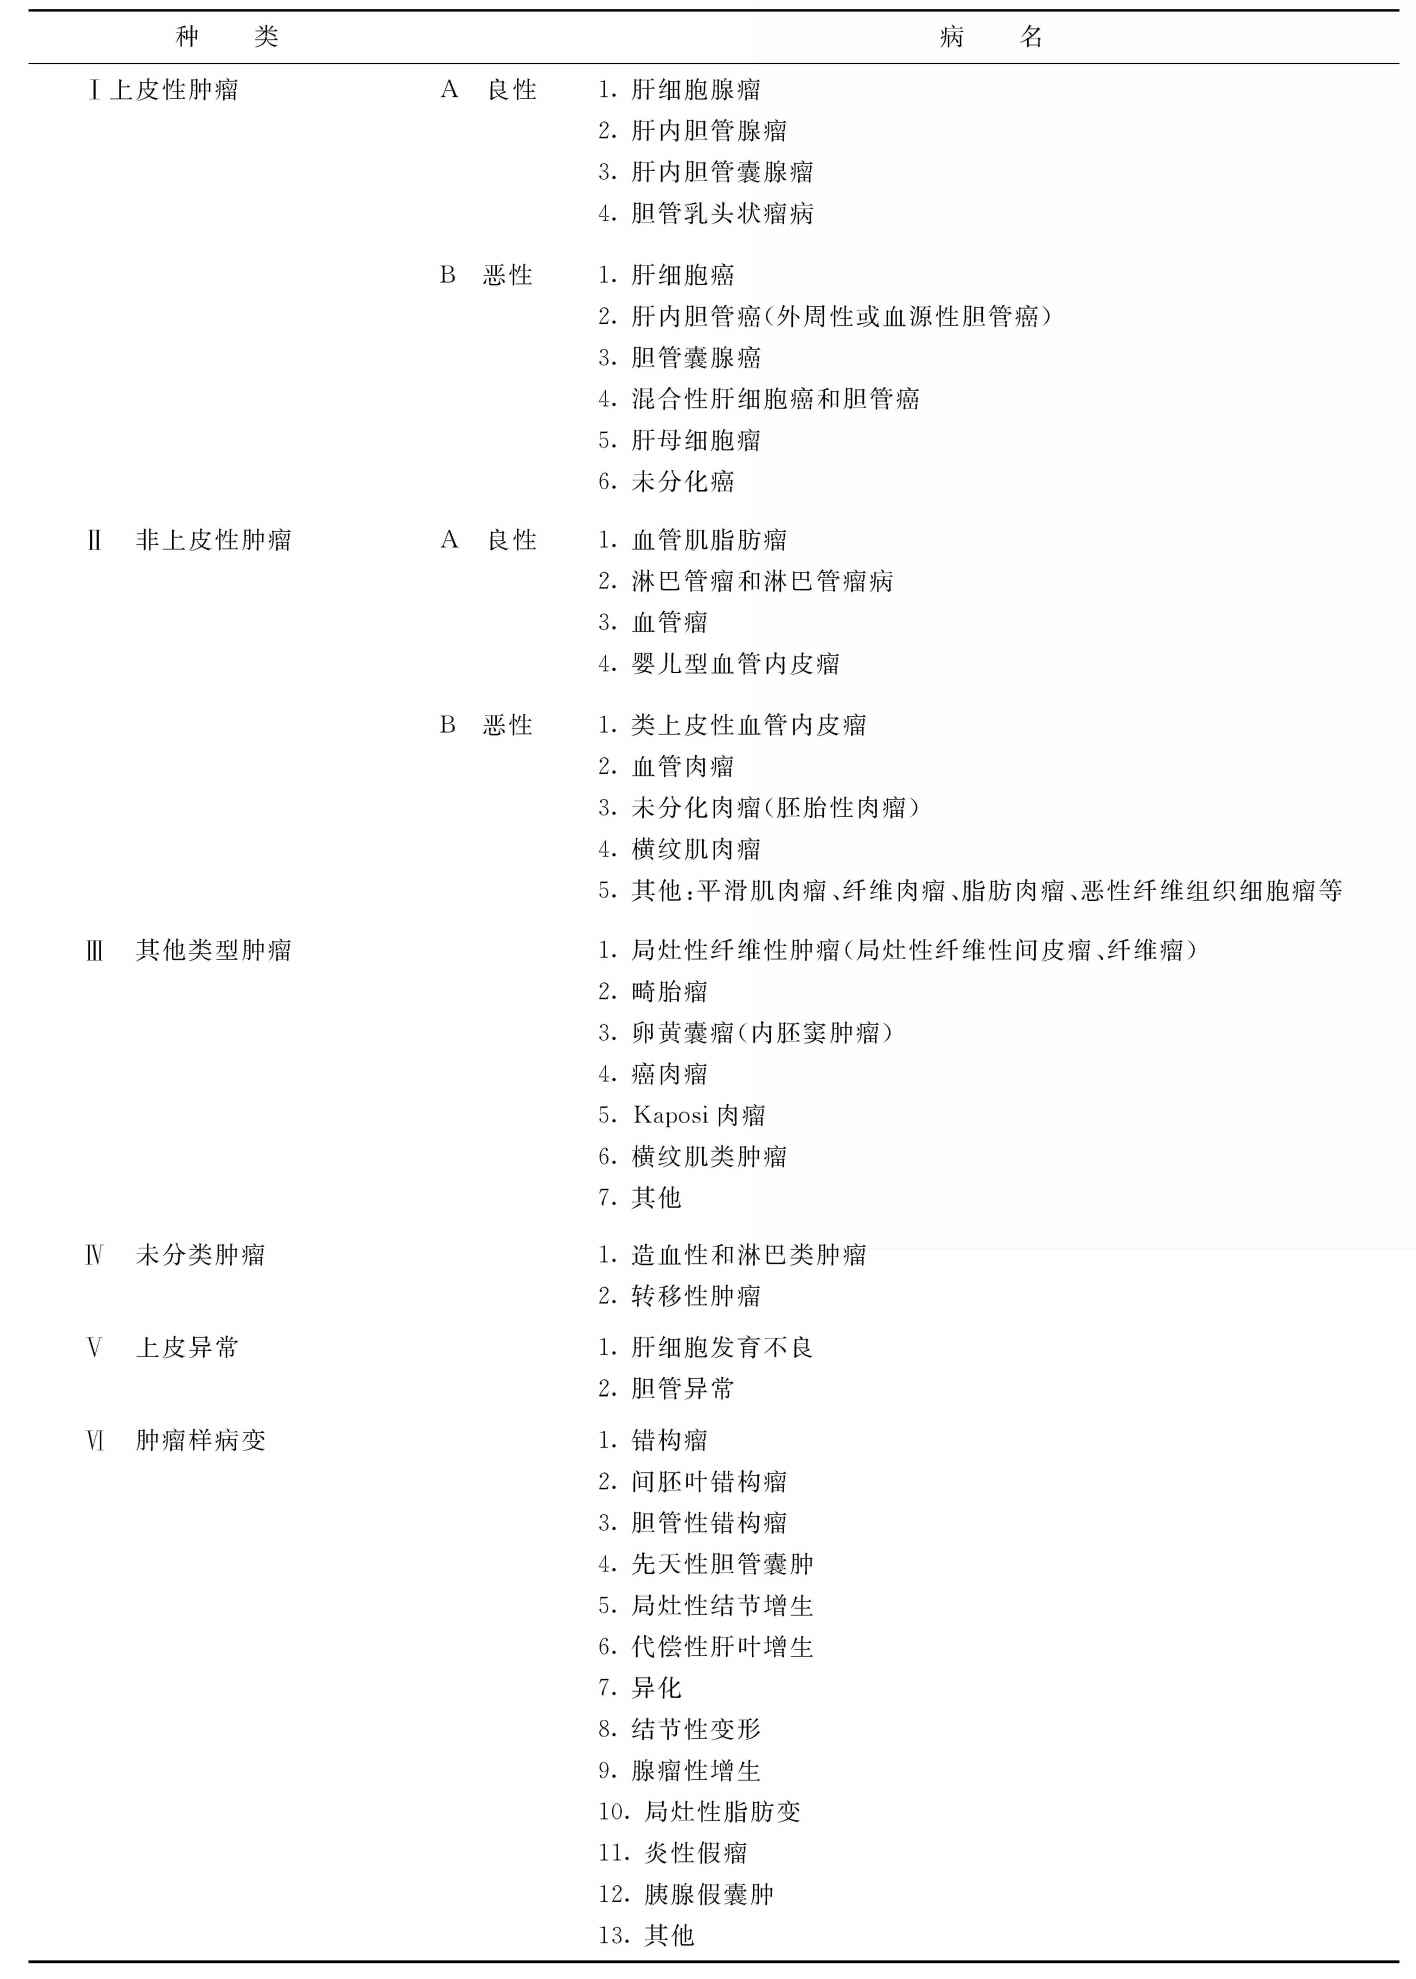
\includegraphics[width=\textwidth,height=\textheight,keepaspectratio]{./images/Image00271.jpg}
\end{table}

原发性肝癌的细胞学类型有:肝细胞癌、胆管细胞癌与混合型。近些年报道的纤维板层样肝细胞癌为肝细胞癌的一种特殊类型。

\subsection{病因}

肝细胞癌的病因主要有两方面。①乙型肝炎病毒(HBV):国内病例中,90%以上感染过HBV,即HBsAg阳性;②黄曲霉素(AFT):长期低剂量或短期大剂量摄入可诱发。此外,与饮水污染、丙型肝炎、戊型肝炎、饮酒和吸烟等也有一定关系。

\subsection{病理}

\subsubsection{肝细胞癌的分级}

可分为4级:Ⅰ级高度分化;Ⅱ~Ⅲ级中度分化;Ⅳ级为低度分化。中度分化最多,其AFP多为阳性,而高度与低度分化者AFP阴性者为多。

\subsubsection{大体病理}

肝细胞癌(HCC)的大体病理分型较为繁杂。

1.Eggel于1901年提出的经典分类曾被广泛应用至今。此分类将HCC分为3型:①结节型:直径<5cm的属结节,单个或多个分布;②巨块型:直径≥5cm,常为单个巨块,也有密集结节融合而成的巨块,以及2个以上巨块的;③弥漫型:少见,该型结节很小,直径约5~10mm,弥漫分布且较均匀,全部合并肝硬化;易与肝硬化结节混淆。上述分类属中、晚期肝癌的类型。

2.70年代以后国内将HCC分为4型:①块状型:单块状、融合块状或多块状;②结节型:单结节、融合结节、多结节;③弥漫型;④小癌型。小癌型(即小肝癌)的提出标志着肝癌诊断水平的提高。

3.80年代以来日本学者的分类为:①膨胀型:肿瘤分界清楚,有纤维包膜(假包膜),常伴肝硬化;其亚型有单结节型和多结节型;②浸润型:肿瘤边界不清,多不伴肝硬化;③混合型(浸润、膨胀):分单结节和多结节两个亚型;④弥漫型;⑤特殊型:如带蒂外生型、肝内门静脉癌栓形成而见不到实质癌块、硬化型肝细胞癌等。日本和中国以膨胀型为多,北美以浸润型为多,而南非地区多不伴肝硬化。国内80%~90%伴肝硬化,而出现相应影像学表现。

4.小肝癌的病理诊断标准:目前国际上尚无统一标准。中国肝癌病理协作组的标准是:单个癌结节最大直径≤3cm;多个癌结节,数目不超过2个,其最大直径总和应≤3cm。

\subsubsection{转移途径}

①血行转移:最常见。HCC易侵犯血窦,在门静脉和肝静脉内形成癌栓,并向肝内、外转移。肺为肝外转移的主要部位,其他有肾上腺、骨、肾、脾和脑等。②淋巴转移:以肝门淋巴结最常见,其次为胰头周围、腹膜后(主动脉旁)和脾门等区域。③种植性转移:最少见。此外,除晚期少数患者产生癌性腹膜炎外,极少发生腹膜转移。

\subsubsection{HCC的单中心与多中心起源}

多结节型HCC或巨块结节型HCC,究竟是HCC肝内播散的结果(即单中心起源)还是多中心起源,尚有争论。Esumi(1986年)通过HBV-DNA整合这一分子生物学方法证实两种可能性同时存在。

\subsection{临床表现}

国内将其临床分为3期:Ⅰ期(亚临床期,无临床症状和体征)、Ⅱ期(中期)、Ⅲ期(晚期)。一旦出现症状,肿瘤多较大,已属中晚期。

1.症状:以肝区痛、腹胀、上腹部肿块、纳差、消瘦、乏力等最为常见,其次可有发热、腹泻、黄疸、腹水和出血等表现,低血糖与红细胞增多症为少见表现。

2.并发症:①肝癌结节破裂出血;②消化道出血,由肝硬化门脉高压和凝血功能障碍所致;③肝昏迷。

3.实验室检查:①AFP(甲胎球蛋白)定量:放免法测定\textgreater{}500μg/L,持续1个月;②AFP
200~500μg/L,持续2个月,并排除其他AFP升高的因素,如活动性肝病、妊娠和胚胎性肿瘤等。小肝癌病例AFP常轻度或中度升高,如持续时间长(低浓度持续阳性)亦应警惕;但有10%~30%的肝癌AFP阴性。其他如γ-GT和各种血清酶测定亦有一定意义。

\subsection{CT表现}

\subsubsection{平扫表现}

平扫很少能显示出<1cm的病灶。肿瘤一般呈低密度改变;少数与周围肝组织呈等密度(分化好的),如无边缘轮廓的局限突出,则很难发现病变;极少数呈高密度(图\ref{fig11-1}A)。当合并脂肪肝时,与肝实质呈等密度及高密度者为肝细胞癌的特征性所见。肿瘤内产生钙化的约占5%以下,还偶见出血及脂肪成分。合并肝硬化者可出现相应表现。

1.结节型:①为单结节或多结节,多呈类圆形;②界限清楚,部分可见完整或不完整的更低密度环状带即假包膜;③肿瘤内常形成间壁而密度不均,另因肿瘤缺血、坏死其内可见更低密度区;④有时肿瘤所在的肝段呈低密度,是由于肿瘤浸润并压迫门静脉血流减少,而致瘤周肝实质营养障碍。

2.巨块型:①单个或多个,占据一叶或一叶之大部分(图\ref{fig11-1});②常因向周围浸润而边缘不规则;③肿瘤内多有缺血、坏死而有不规则更低密度区;④周围常有子灶(<5cm为结节),有人称之巨块结节型。

3.弥漫型:平扫难以显示弥漫的小结节。可见肝脏呈弥漫性增大、肝硬化以及门静脉内瘤栓形成(图\ref{fig11-2})。

\subsubsection{增强扫描}

肝癌主要由肝动脉供血,但几乎都存在着不同程度和不同情形的门静脉供血。早期肿瘤血供多来自门静脉,随着肿瘤发展,动脉供血逐渐成为主要血供,而门静脉供血逐渐走向瘤周。CT增强表现为:

1.动脉期:肿瘤显著强化(图\ref{fig11-1}B)。小肝癌常为均一强化;大肝癌由于内部形成间壁、有不同的血管结构、缺血坏死等而呈不均匀强化。但有时小肝癌动脉期不强化(国内有人统计占13.2%),主要与其坏死有关,透明细胞变可能是另一原因。

2.门静脉期:肿瘤呈低密度改变(图\ref{fig11-1}C)。此时,病变范围比平扫时略缩小,边界较为清晰。是因为肝癌90%~99%由肝动脉供血,而周围肝实质约80%由门静脉供血,两者增强效应时相不同所致。

3.平衡期:肿瘤仍呈低密度(图\ref{fig11-1}D)。如与血管瘤鉴别可延迟至7~15min扫描(即所谓延迟扫描)仍呈低密度。

\begin{figure}[!htbp]
 \centering
 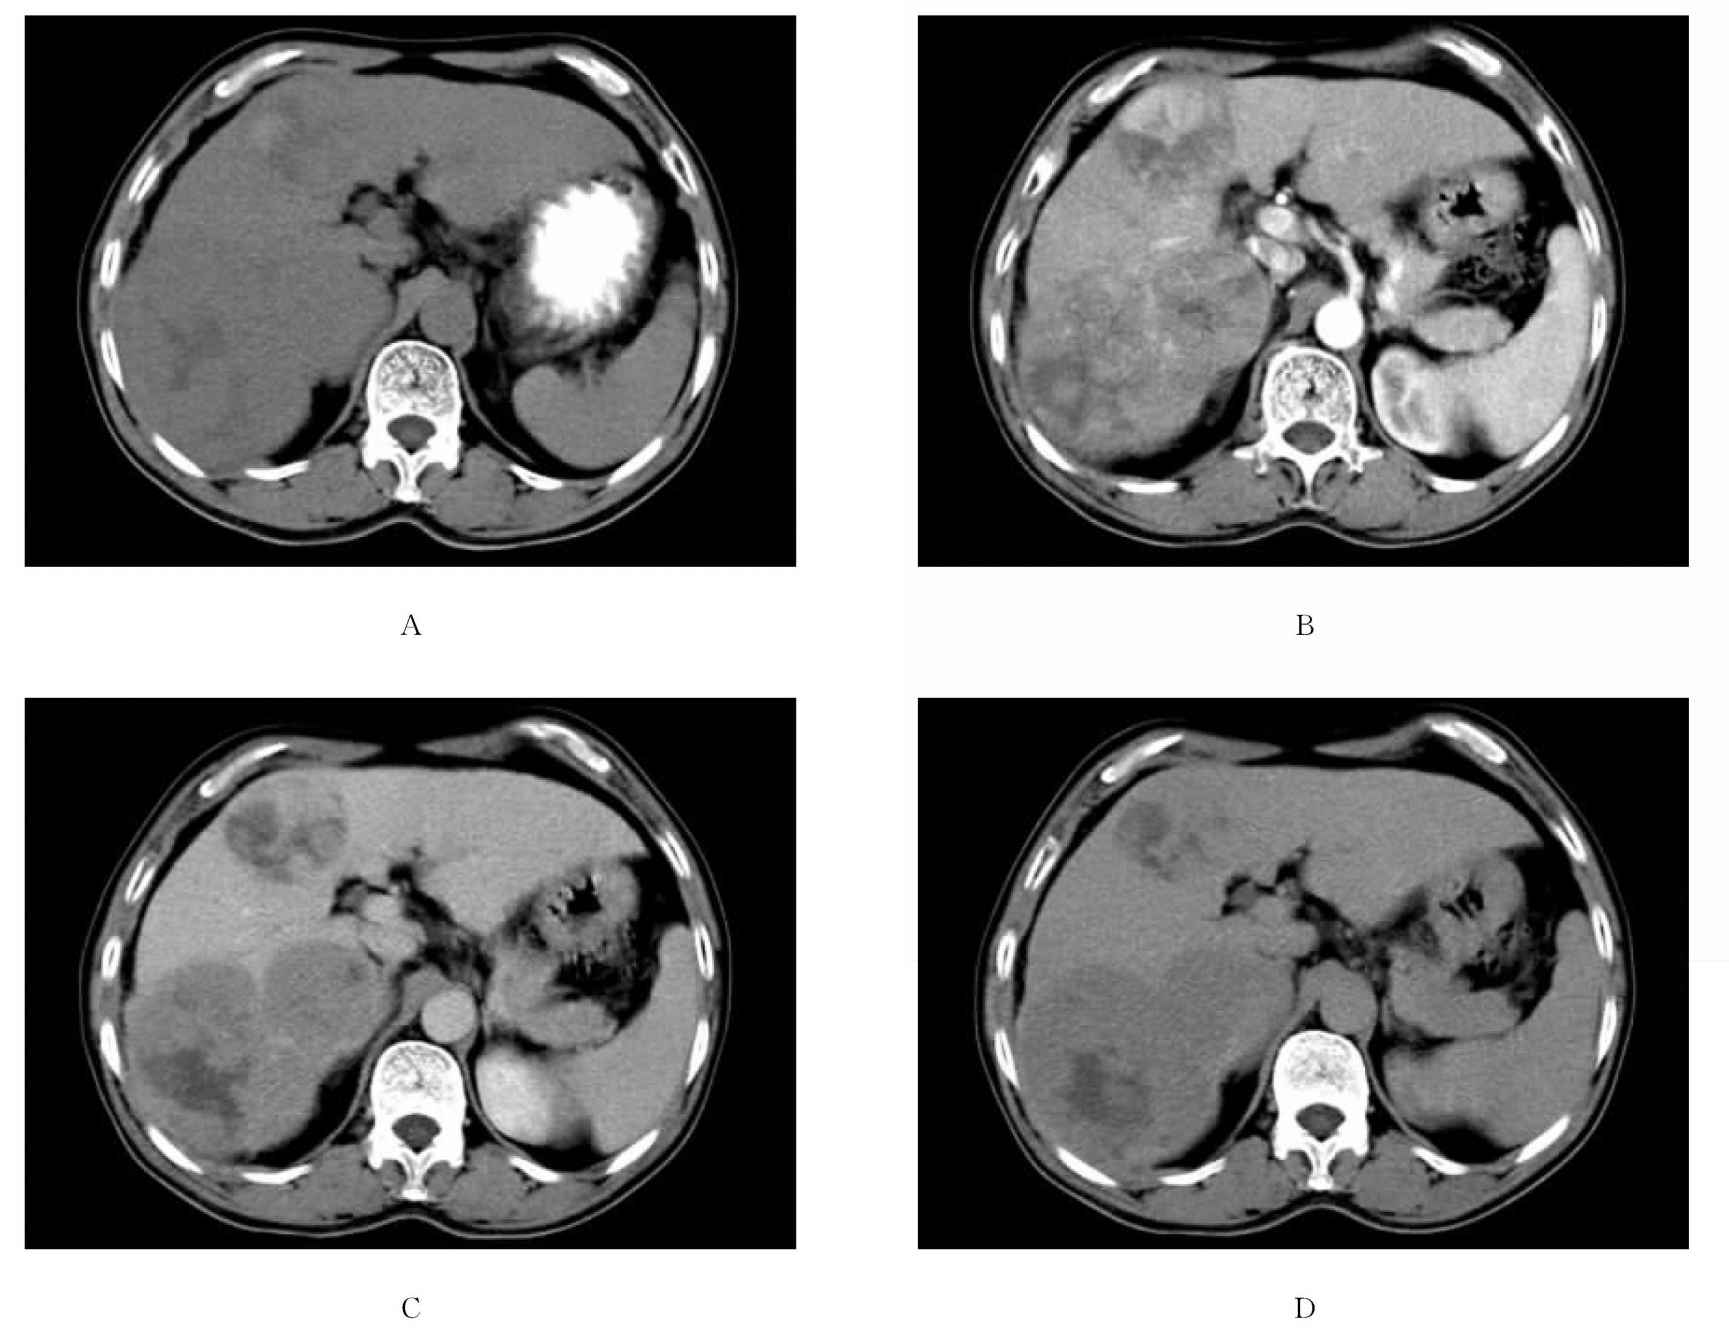
\includegraphics[width=.7\textwidth,height=\textheight,keepaspectratio]{./images/Image00272.jpg}
 \captionsetup{justification=centering}
 \caption{肝癌(巨块型)\\{\small A~D为同一患者。A.平扫可见干左右叶有团块状等、低、高混杂密度灶,界限欠清晰;B.动脉期病灶部分有强化,病灶界限清晰;C.门静脉期病灶呈低密度,界限清晰,其内有更低密度的坏死区;D.平衡期病灶呈低密度}}
 \label{fig11-1}
  \end{figure} 

\begin{figure}[!htbp]
 \centering
 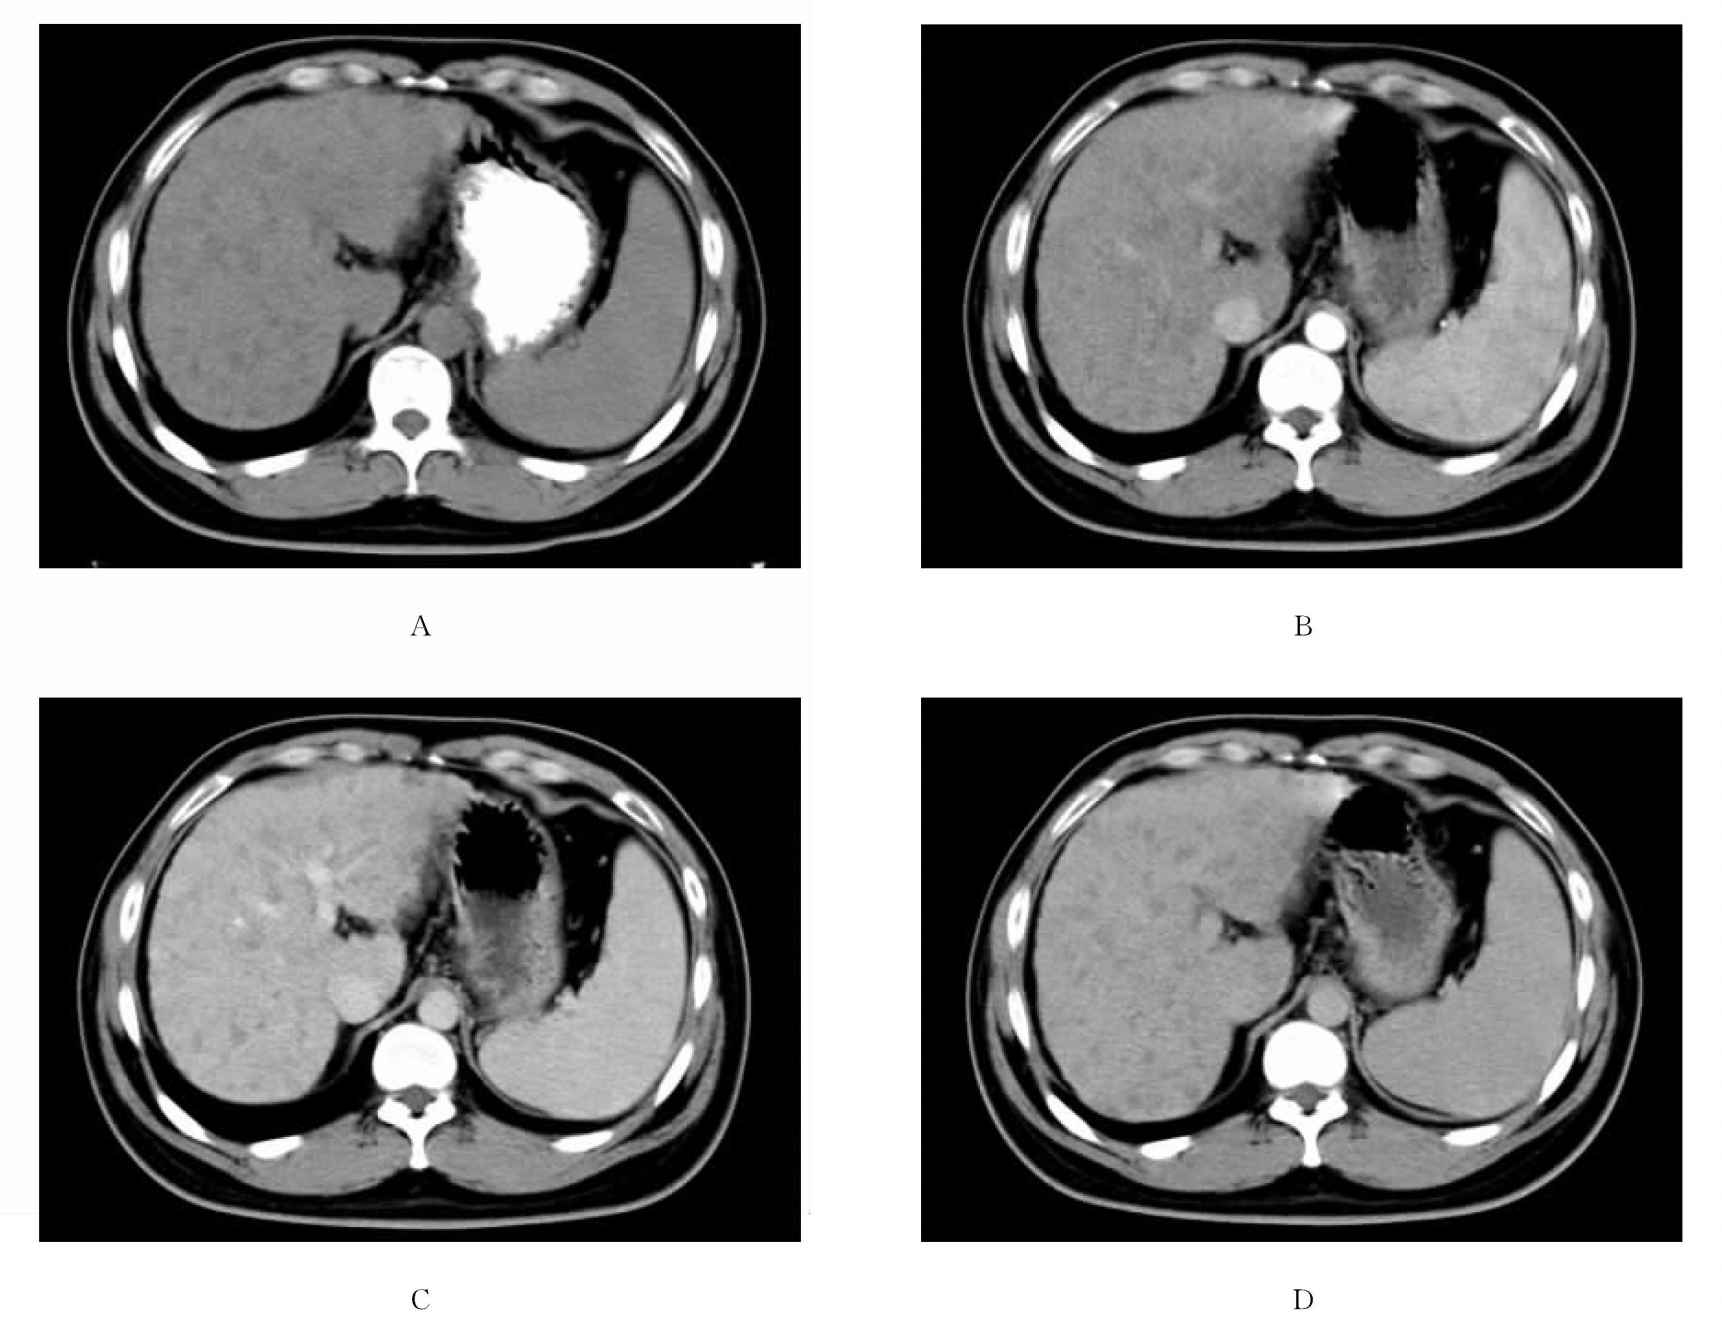
\includegraphics[width=.7\textwidth,height=\textheight,keepaspectratio]{./images/Image00273.jpg}
 \captionsetup{justification=centering}
 \caption{肝癌(弥漫型)\\{\small 分别为平扫和三期增强扫描;肝内弥漫性分布有许多低密度小结节}}
 \label{fig11-2}
  \end{figure} 

\subsubsection{CT增强的时间-密度曲线}

肝癌CT增强的时间-密度曲线可分为5型:①速升速降型;②速升缓降型;③无明显变化型;④速降缓升型;⑤初期速降而后稳定极缓上升型。但速升速降型是其特征性强化表现。

因肝癌主要由肝动脉供血,在动脉期CT值迅速上升达到峰值并超过肝实质。因平扫病灶密度多低于肝脏,故在其密度升高的极早期有一次与肝实质密度相近的第一次等密度交叉,但因极短暂,故一般不会显示。病灶峰值停留的时间很短,然后迅速下降,随着肝实质的CT值上升,两者的密度接近出现第二次等密度交叉。此后病灶密度缓慢下降而正常肝实质密度继续上升,病灶又成为低密度。但正常肝实质的增强上升速度较肝癌缓慢,达到的峰值低,峰值停留时间长,下降速度不及肝癌。

总之,凡血供丰富的HCC,与正常肝实质对照均出现从高密度、等密度到低密度的3步曲,整个过程短暂,时间密度曲线呈速升速降型,这是肝癌的特征性表现。可能由于乏血、门静脉参与血供较著等,因而出现其他4种强化曲线。

\subsubsection{肝细胞癌的包膜及其边缘强化方式}

1.纤维包膜的形成:是由于肿瘤呈膨胀性生长,对邻近的非癌变肝组织产生压迫,引起纤维结缔组织增生;同时由于肿瘤细胞及其间质细胞产生促进血管生长的细胞因子,使纤维结缔组织内形成数量不等的血管。此外,癌灶压迫周围正常肝组织,进一步有利于包膜的形成。

2.HCC的边缘强化方式:①动脉期未显示明确包膜,门脉期和平衡期显示明确包膜呈高密度影,提示肿瘤呈膨胀性生长,且包膜血管较少;或确无包膜,但癌周受压肝组织仍由门静脉供血而呈线环状强化。②动脉期包膜呈低密度,门静脉期和平衡期显示明确的包膜(略低或高密度)或包膜不清,提示肿瘤呈膨胀性生长,包膜内血管少。③三期扫描均见明确包膜且呈环状或不完整环状的高密度强化,提示包膜血管丰富。④动脉、门脉期未见包膜显示,平衡期显示包膜呈高密度,包膜内血管少。⑤三期扫描均未显示明确包膜,表现为癌灶与非癌变肝组织分界不清,提示肿瘤呈侵袭性生长,且生长迅速,无纤维结缔组织包膜。

国内有学者认为,HCC分化低者以不完整环状强化为主;分化高者以完整环状强化为主。

\subsubsection{及与肝硬化、血管瘤APVS的形成机制的区别}

国内有学者将APVS的动脉期表现分为3型:①Ⅰ型:门静脉三级(亚段)及以上分支提早显影;②Ⅱ型:肿瘤或病变周围肝实质提早强化;③Ⅲ型:肝脏边缘结节形、楔形提早强化,且邻近无占位性病变。此外,还有文献报道少见的弥漫型,表现为全肝早期强化,门静脉早显。

1.肝癌:肝癌病灶内出现动静脉分流征象为肝癌的特征之一。其APVS的发生机制有以下3种。①跨血管的APVS:即肿瘤组织对门静脉分支的直接侵犯破坏,使肿瘤处的肝动脉血通过破坏的门静脉壁直接灌入门静脉分支,形成肿瘤性APVS。CT表现为Ⅰ和Ⅱ型。②跨肝窦的APVS:肿瘤组织压迫、侵犯周围的肝静脉分支,造成该区域肝静脉回流受阻,致使肝窦压力升高,当此压力超过门静脉压力时,所属门静脉就成为引流静脉,直接接受肝动脉血液,形成跨肝窦的APVS。又由于受累区功能性门静脉血流减少,而致肝动脉的血流代偿性增加。还有人认为,在压迫肝静脉的情况下肿瘤周围的肝实质还会“盗取”肿瘤组织的肝动脉血供。该类在CT上呈Ⅱ型表现。③跨血管丛的APVS:肿瘤的压迫和(或)门静脉较大分支的瘤栓都可造成门静脉血流受阻,此时位于肝脏中央部分较大胆管的周围血管丛作为顺肝方向的侧支循环开放、增生,代偿受阻的门静脉血流。这种APVS在CT亦表现为Ⅱ型。但肝癌所致的Ⅱ型病变在门静脉期和平衡期均不呈低密度,有助于与肿瘤子灶相鉴别。

2.肝硬化:其APVS的CT表现以Ⅲ型多见。其形成主要与肝硬化时继发肝内血管网结构的扭曲、肝窦微细结构的变化以及门静脉高压等变化有关。原因可能为:①跨肝窦的APVS:因肝窦的结构会出现毛细血管化、胶原化,其通透性也有变化,肝内血管网结构的扭曲可使小的肝静脉出现梗阻,从而形成跨肝窦的APVS;②跨血管丛的APVS:门脉高压所致,与上述肝癌APVS的形成机制相似;③跨血管的APVS:尚未见报道,但国外有学者电镜发现肝硬化的大鼠可出现。

3.血管瘤:有文献报道肝海绵状血管瘤有近23.5%~29.7%出现APVS。于动脉期表现为瘤周楔形强化区(Ⅱ型),常伴门静脉支早显。随着时间的延长有的可变为低密度,最后呈等密度。伴脂肪肝时于平扫图上即可见到与异常灌注类似的高密度影。从狭义上说这种瘤周楔形强化区是指瘤旁肝组织内那些与瘤体内血窦相通的、扩大的肝窦腔隙或异常薄壁血管腔被对比剂充盈所致,从广义上可认为这种楔形强化是血管瘤并发APVS的一种特征性表现。

总之,APVS以肝癌最为多见,且CT表现为Ⅰ、Ⅱ型;亦可见于单纯肝硬化者,而其CT表现以Ⅲ型多见;血管瘤所致APVS应予重视。此外,肝转移瘤、肝脏手术、穿刺后亦可发生,偶为正常人。APVS应注意与肝第3血供所致的假性病变相鉴别。

\subsubsection{肝脏灌注异常}

导致肝脏灌注异常的病因:多种多样,包括门静脉阻塞(癌栓、血栓)、肝静脉阻塞(布加综合征、心衰、纵隔纤维化等)、局限性肝脏病变、感染(肝脓肿、胆囊炎、胆管炎)、肝内门-体分流术后所致的血流动力学改变、肝脏肿瘤、肝硬化、急性胰腺炎等,以及已述及的第3血供。

门静脉癌栓所致的肝灌注异常的增强CT表现:动脉期的不规则形或三角形高密度区,或(和)门脉期不规则形或三角形低密度区。

门静脉癌栓所致的肝实质灌注异常,其部位与受累门静脉分布一致。但当合并动脉-门静脉短路时则例外。其形成机制为:①门脉癌栓形成后血流受阻,致相应区域肝实质门静脉血供减少,即门静脉血流灌注减少。为维持肝实质血流量的相对恒定,则供应该区域的肝动脉血流量将代偿性增多,即动脉血流量高灌注。我们认为,从前已述及肝动脉-门静脉分流(APVS)之跨血管丛型可知,这种灌注异常还可与APVS有关。②门静脉期低灌注(伴或不伴动脉期高灌注),可能原因有两方面:一是由于门静脉癌栓未导致管腔完全阻塞,仍有血流通过肝实质;二是由于脾静脉与肝内门静脉分支之间存在着较广泛的侧支循环,这些侧支循环开放(即门静脉海绵样变),使门静脉属支的血液绕过癌栓阻塞的部位进入肝脏。

\subsubsection{门静脉海绵样变}

门静脉海绵样变(CTPV)是指门静脉栓塞或后天性、先天性狭窄后引起门静脉旁、肝内及胆囊窝小静脉或毛细血管呈网状扩张,以及栓塞的门静脉再通。

正常情况下门静脉周围仅见肝固有动脉伴行,极少数可见门静脉周围有2~3个小血管断面显示,可能是胃右动脉或胆囊动脉显影,或存在解剖变异。胆囊壁及周缘无肉眼可见的小血管断面。故国内有学者提出CT图像以门静脉周围血管横断面多于3个作为胆总管周围侧支循环开放的标准。

门静脉癌栓所致的位于肝门、肝十二指肠韧带的形似海绵的静脉网,由门静脉之间的侧支循环(门-门短路)和门静脉分流至体循环(门-体分流)的侧支循环所形成。它包括:①门静脉胆支:包括胆囊静脉和胆管周围静脉丛;②门静脉胃支:包括胃左静脉(即胃冠状静脉)、胃右静脉,以及它们的属支如食管静脉、胃短静脉、幽门前静脉和幽门十二指肠静脉;③胰十二指肠后上静脉;④脐旁静脉:其扩张提示门体分流的存在。

国内文献报道,门静脉胆支和胃支是构成门脉海绵状变的最主要血管;胆支开放仅见于门脉海绵样变(但有学者认为亦可见于肝硬化);胰十二指肠后上静脉亦较常显示;门静脉胃支的开放与肝硬化并门静脉高压,以及门脉海绵样变均有关系。

\subsubsection{门静脉、肝静脉、下腔静脉癌栓和门静脉动脉化征}

肝细胞癌向门静脉、肝静脉、下腔静脉浸润生长时,可形成肿瘤癌栓。

1.门静脉内癌栓:①平扫癌栓的密度与门脉血液密度无差异,但受累血管因癌栓生长有扩大,造成分支直径大于主干或主干与分支粗细不成比例。②增强后表现为血管内充盈缺损征象,相应血管扩张。③增强后动脉早期癌栓强化及其内显示细小的肿瘤血管,称为“门静脉动脉化征”,其发生率可高达86%,是与血栓鉴别的主要征象。血栓一般主要位于肝外门脉,累及或不累及肝内主干及分支。④位于末梢的门静脉癌栓诊断困难,CTAP有利于显示,并可见此范围呈扇形低密度区。

2.肝静脉和下腔静脉受侵和癌栓:①受侵犯的血管不规则狭窄,或见局部压迹,也有完全被肿瘤包绕的;②腔内充盈缺损,个别病例向上可延伸至右心房内;③局部管腔扩大;④奇静脉、半奇静脉扩张;⑤应注意:增强扫描早期下腔静脉可部分显影或密度不均,需同一部位重复扫描鉴别;下腔静脉受肿块压迫亦可不显影。

\subsubsection{肝细胞癌胆管内浸润}

据统计,肝细胞癌伴有肝内胆管扩张的发生率为14.4%,小肿瘤很少发生,是肝癌肿块的直接压迫、侵犯或肝门区转移淋巴结压迫所致。肿瘤向胆管内直接浸润生长,可形成胆管内癌栓,比较少见,其发生率约在13%左右,多同时合并门静脉及肝静脉内癌栓。

CT表现:肝内胆管轻、中度扩张,以肝门(包括左、右肝管)附近多见。CT可显示肝总管或大分支内癌栓,确诊需胆道造影。对于末梢部位者,一般形成胆管内癌栓之肝细胞癌多属乏血型,周围又有扩张的胆管,故应与肝内胆管细胞癌鉴别。直接显示出胆管内癌栓及伴随门静脉癌栓征象对诊断和鉴别极为重要。

\subsubsection{肝细胞癌肝内转移的方式}

其肝内转移方式有两种。①门静脉性:癌细胞经肿瘤周围之门静脉系,着重于末梢侧或中枢侧之肝实质内形成转移灶。若合并肝门侧的动脉-门静脉短路,可转移至肝较远部位。②肝动脉性:多由其他脏器的肝细胞癌转移灶,再循环入肝动脉血,引起肝动脉性肝内转移,此种方式只见于晚期患者。

CT表现:肝内均一大小转移灶,易发生在肝被膜部位。结节型和巨块型均可伴有肝内转移,也称为子结节。平扫及增强扫描病变特点与原发灶基本相同。

\subsubsection{肝细胞癌破裂出血}

其CT表现为:平扫示肿瘤内斑片状、片状高密度灶;也可表现腹腔内广泛出血;还可形成肝包膜下血肿,呈沿肝脏表面的月牙形、梭形血肿征象。

\subsubsection{肝细胞癌肝外浸润及转移}

1.肝细胞癌向周围邻近脏器直接浸润极少。①病灶巨大或近横膈者可产生横膈的直接浸润,并进而浸润胸腔。但除晚期患者外,极为少见。②肝左叶与胃前壁相邻,但肝癌直接浸润胃的发生率极低。③肝镰状韧带及胆囊可有直接受侵,也极少见。

2.肝细胞癌早期远隔转移少见,晚期可发生血行转移、淋巴转移及腹膜种植转移。

\subsection{肝纤维板层样癌}

肝纤维板层样癌(FL-HCC)是肝细胞癌的一个罕见和特殊类型,约占肝细胞癌的1%~2%。

\textbf{【病理】}
以左叶多见,常单发。肿块呈膨胀性生长、体积较大、包膜完整,常伴明显纤维组织包绕,肿瘤内部可见钙化。显微镜下肿瘤细胞呈多边形;纤维基质成分较多,有时排列较整齐,将肿瘤细胞分隔成条带状或团状,有一定特征性。

\textbf{【临床表现】}
可发生于任何年龄,但好发于青年人。男女发病率相近。以腹块和上腹部不适为主,通常无病毒性肝炎或肝硬化病史。实验室检查如HBsAg阴性,AFP、CEA、AKP等均正常或略增高。本病手术切除预后好。

\textbf{【CT表现】}
平扫病灶为边缘较清楚的低密度区,可显示内部更低密度的条索状区和坏死区。病灶内出现点状、小圆形钙化为其特点。病灶周围有时可见卫星灶。肿瘤实质部分富血供,增强扫描与传统的肝癌表现相似。动脉期呈早期增强表现,而纤维间隔则为相对低密度。继发改变有肝内胆管扩张、血管受压或侵犯等,但极少有动脉-门静脉短路及门静脉内癌栓形成。

总之,其CT表现无特异性,但在年轻和无肝硬化的患者中,若发现肝内巨大肿块,除外血管瘤后,应考虑到FL-HCC的可能。但应注意与肝局灶性结节增生(FNH)鉴别。

\subsection{鉴别诊断}

\subsubsection{血管瘤}

血管瘤表现典型,两者多鉴别不难,但小血管瘤的变化较多。注意快速推注造影剂于动脉早期快速扫描,以及充分的延迟扫描有助于诊断。血管瘤有以下CT特点:①平扫呈类圆形低密度,密度多均匀、边缘清晰;②增强扫描于动脉早期出现边缘结节状、点状、斑点状等显著强化,其密度可与同层腹主动脉相近,有特征性;且密度高于周围肝实质的持续时间即强化峰值持续时间长,超过2min;③增强区域进行性向病灶中央扩散;④延迟扫描病灶呈等密度充填;⑤如病灶中央有纤维瘢痕,除瘢痕不强化外,增强扫描仍符合上述特点;⑥少数病灶强化不著,但延迟期仍呈等密度充填;⑦个别病例始终无强化,延迟扫描亦无充填则诊断和鉴别诊断困难。

\subsubsection{肝转移瘤}

转移瘤有以下CT特点:①转移瘤病灶多发、散在、大小相仿;②少血供者明显的边缘强化和“牛眼征”;而少数富血供者呈弥漫性强化;③较小病灶出现囊样变伴边缘强化;④无门脉癌栓和病灶周围的包膜(或晕圈)显示;⑤邻近脏器发现原发灶、复发灶或转移灶。

单个或数目不多的转移灶与HCC鉴别有一定困难。①大小不一,特别是大病灶周围的结节(卫星灶)形式出现以HCC可能大;②增强扫描病灶呈速升速降改变的以HCC可能大;而转移瘤门静脉期可呈渐进性厚壁强化,但强化程度低于肝组织;③病灶周围有包膜及门脉癌栓形成明显支持HCC;④两者大的瘤灶均可出现囊样坏死,而小瘤内囊样变一般不见于HCC。

\subsubsection{肝内胆管细胞癌}

肝内胆管细胞癌CT表现无特异性,下列特点有助于与肝癌鉴别。①呈边缘欠清的低密度灶,病灶常较大,部分病灶有点状钙化;②肿瘤多乏血,增强早期及门静脉期可见肿瘤边缘轻度不连续环状强化;③国内有学者报道近60%的病例可出现瘤体延迟强化;④局部肝内胆管扩张较多;极少数有门静脉侵犯或癌栓形成;⑤极少数有肝硬化表现,AFP为阴性。

总之,如病灶较大,且其内有点状钙化或大片状的无强化的液性密度区出现时,应考虑胆管细胞癌。肿瘤边缘不连续环状强化及低密度肿瘤内含无定形的稍高密度影是其双期增强扫描的典型表现。

\subsubsection{肝硬化结节}

单个或多个肝硬化结节与肝癌结节很难鉴别。

1.肝硬化结节缺乏动脉血供。团注动态增强扫描,甚至CTA如病灶无强化,则以再生结节、局灶性脂肪变或坏死结节可能大;结节明显强化则可确立肝癌的诊断;如仅轻度强化,或血管造影见轻度染色,则很难做出诊断。总之,肝动脉血供的有无及程度与结节的良、恶性相关。

2.大结节性肝硬化:肝脏表面高低不平,肝内有许多再生结节,颇像多结节性或弥漫性肝癌。下列征象有助于鉴别:①在平扫图上,肝硬化再生结节较正常肝组织密度略高。②增强扫描结节强化不明显,或不及正常肝组织,故成为低密度;或两者密度趋向一致,肝脏密度由平扫时的不均匀变为均匀。后一种情况更多见,更具有诊断意义。③门脉内见不到癌栓,而弥漫性肝癌的门脉癌栓发生率近于100%。

\subsection{肝硬化再生结节至肝细胞癌的演变}

在肝硬化基础上肝细胞癌的发生是一个多阶段过程,在这一过程中再生结节可能是第一步。其演变过程有两种观点:①再生结节(RN)→腺瘤样增生(AH)或称为普通型AH→不典型腺瘤样增生(AAH)→早期肝细胞癌(EHCC)→小肝细胞癌(SHCC);②RN→发育不良结节(DN)→含局灶癌变的发育不良结节→SHCC。

1.病理特征

(1)再生结节(RN):是在肝硬化的基础上发生局灶性增生而形成的肝实质小岛,直径多在0.3~1.0cm。内含肝细胞、Kupffer细胞及小胆管等正常肝组织,周围被硬化肝脏的粗糙纤维间隔所包绕。

(2)发育不良结节(DN):最初称为腺瘤样增生,还有再生大结节、腺瘤性增生及肝细胞假瘤等名称。1994年国际胃肠道会议正式命名为发育不良结节。结节常>1.0cm,多<2.0cm,可达3.0cm左右。无真正包膜。镜下根据细胞异形性程度又分为低度DN和高度DN,分别相当于腺瘤样增生的普通型AH和AHH。后者细胞异形性较明显,被认为是癌前病变。当DN内部出现癌灶时就称为早期肝细胞癌。

(3)小肝细胞癌(SHCC):其定义无统一标准,国内规定直径≤3cm或两个相邻结节直径之和≤3cm。包膜、脂肪变性及镶嵌模式等都是SHCC较为特征的病理改变。

2.CT表现和区别

(1)平扫:SHCC呈界限清楚的低密度;RN和DN有聚铁特性,偶呈高密度。

(2)动态增强扫描:由RN至SHCC随着结节恶性程度的增高,肝动脉供血比例逐渐增加,而门静脉供血比例逐渐减少并走向结节周围。96%的发育不良结节(DN)主要由门静脉供血,而94%的HCC主要由肝动脉供血。①HCC于动脉期明显增强,而门静脉期又呈低密度;CTA呈高密度,CTAP呈低密度。②RN、DN的血供大部分为门静脉,其增强规律与正常组织多相似;CTA、CTAP亦与肝实质同步。③一些分化较好的SHCC与含癌灶的DN(即早期肝癌)、异形性明显的DN(相当于非典型样腺瘤样增生),其血供无明显差别。因此,三者有一定重叠性,CT表现无特异性,鉴别较困难,需结合MR、US等综合分析。

但对上述由再生结节至小肝细胞癌的演变过程,有时病理亦难以鉴别(图\ref{fig11-3})。

\begin{figure}[!htbp]
 \centering
 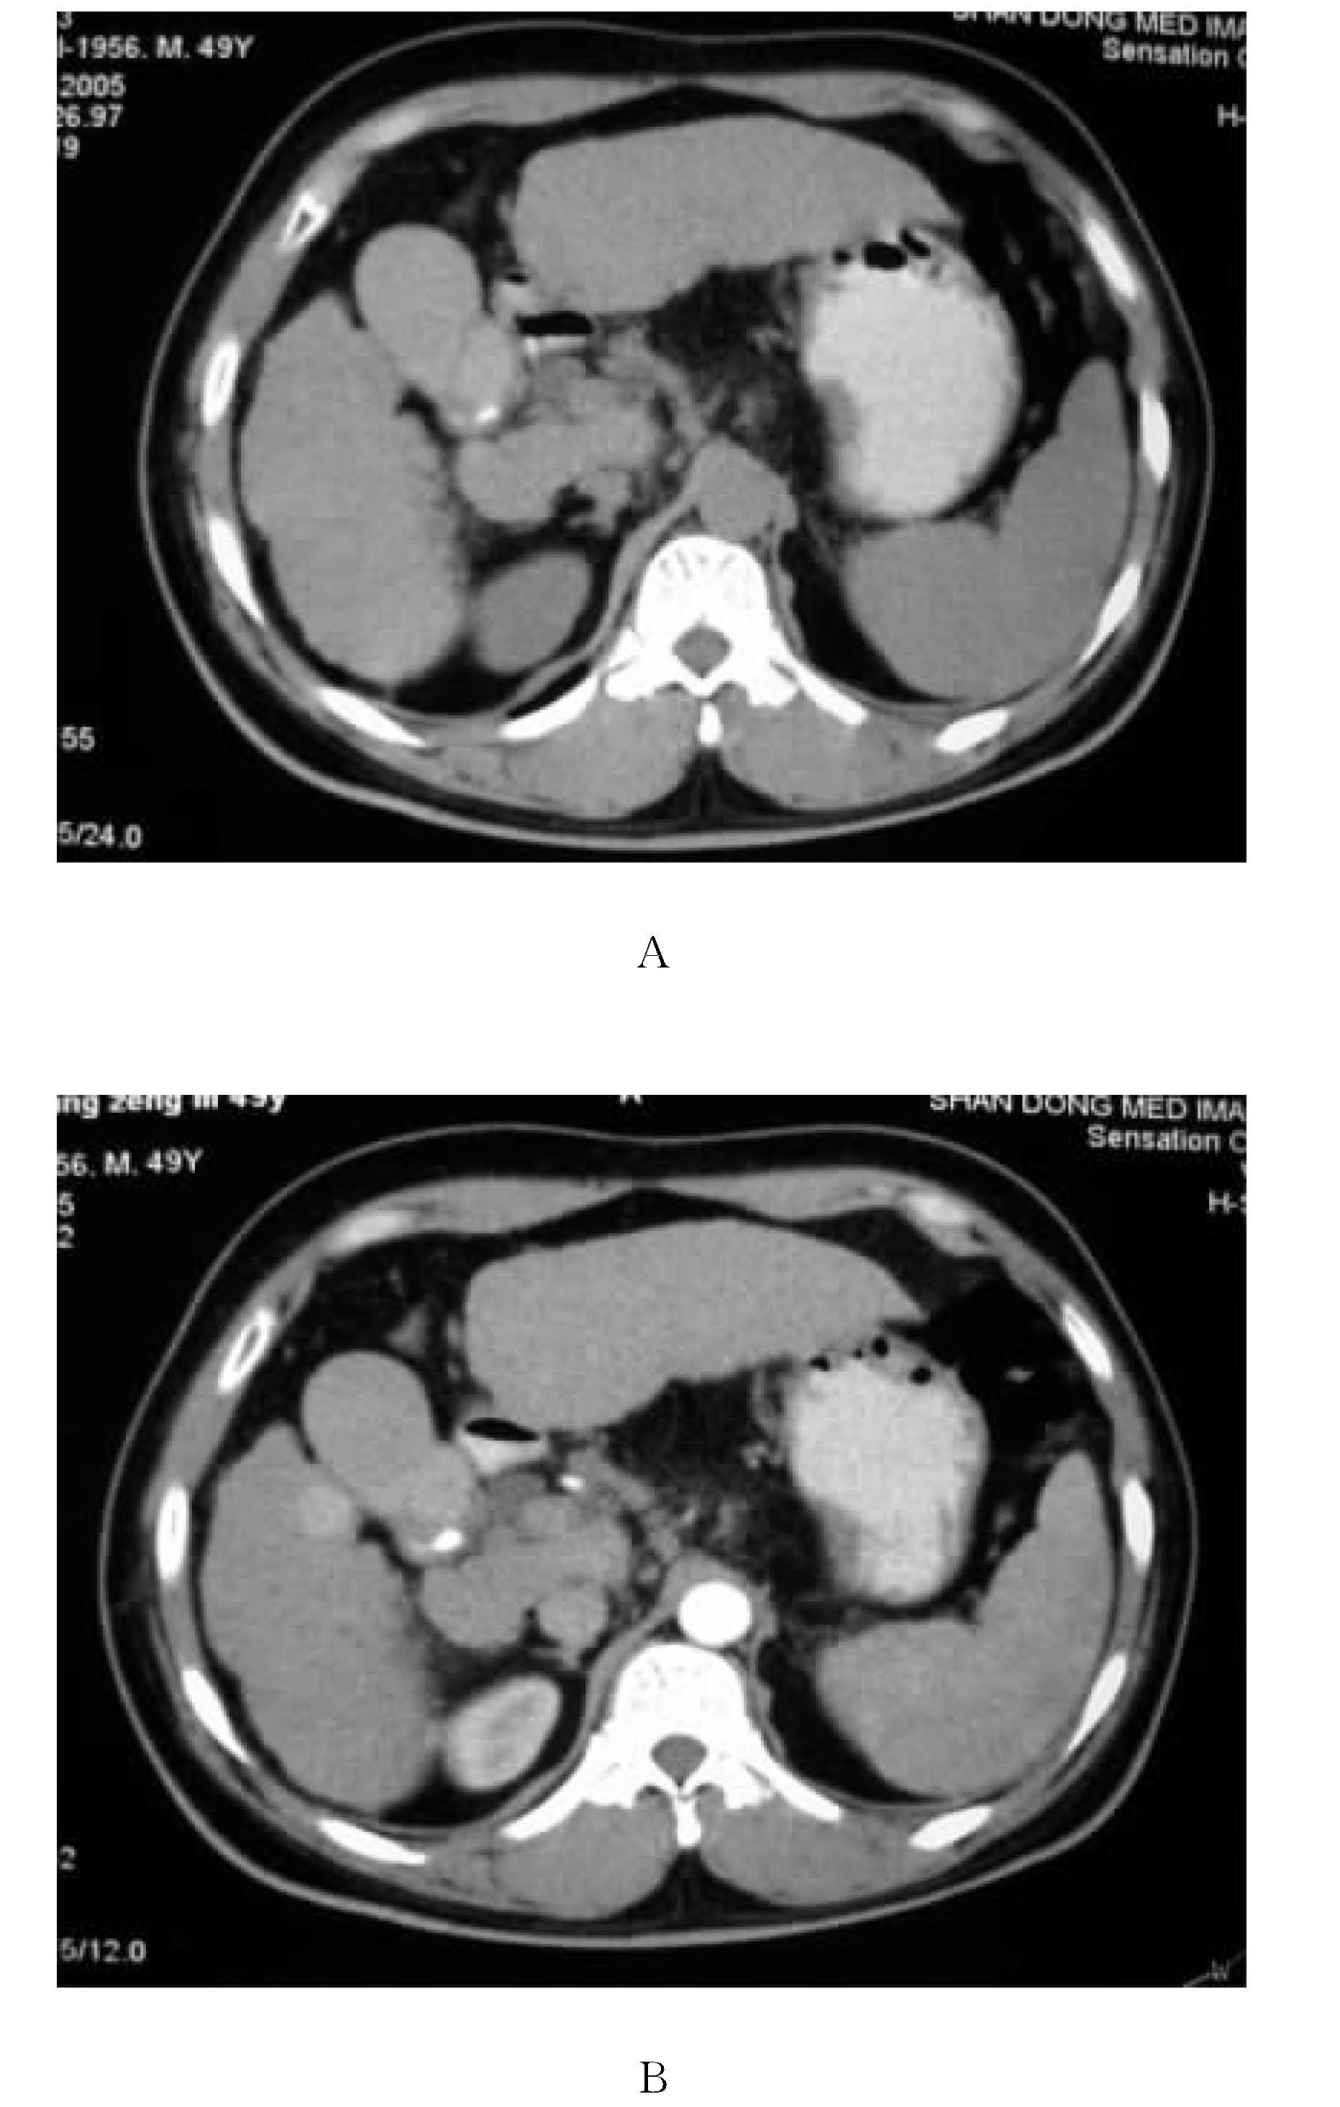
\includegraphics[width=.7\textwidth,height=\textheight,keepaspectratio]{./images/Image00274.jpg}
 \captionsetup{justification=centering}
 \caption{小肝癌(手术证实)\\{\small A、B为同一患者,由肝硬化继发。A.平扫病灶显示不清;B.动脉期病灶呈高密度强化(位于胆囊右侧的肝右叶前下段)}}
 \label{fig11-3}
  \end{figure} 

\subsection{肝癌术后复发及鉴别诊断}

1.肝癌术后复发的病理机制:①肝内转移和播散;②多中心起源;③术中小的病灶未被发现,而后继续生长。

术后AFP浓度未下降到正常,或短期内又复上升;3个月之内又发现新病灶,或原来可疑病灶又增大,通常把它归为术后残存。如术后AFP降到正常,3个月后又复升高,同时找到新病灶通常归为复发灶。复发的时间从3个月至5年不等,也有10年以上的。

2.鉴别诊断:复发灶以结节型、单个居多,与原发灶CT表现基本相同,但需与术后残腔和纤维瘢痕鉴别。①残腔:多呈水样密度,轮廓光滑,无强化;②纤维瘢痕:靠近手术部,平扫呈低密度,无张力和占位效应,边缘较清楚,无明显强化。

\section{非肝细胞性肝脏恶性肿瘤及转移瘤}

\subsection{肝内胆管细胞癌}

本病又称周围型胆管细胞癌,占肝脏原发性恶性肿瘤的第二位。

\textbf{【病理】}
起源于肝内胆管的上皮,如起源于左右肝管或总肝管称为肝外胆管癌。大体标本与肝细胞癌无法鉴别,比肝细胞癌硬,常无肝硬化。组织学表现为腺样分化或伴有黏液分泌,富于纤维性间质,有时可见钙化。肿瘤外周以肿瘤细胞为主,而纤维组织含量较少;中央区则反之。

\textbf{【临床表现】}
本病平均发病年龄50岁左右,男女发病相近或女性稍多见。早期无症状,多以上腹部胀痛不适和肿块为首发症状。还可有间歇性皮肤巩膜黄染、乏力纳差、畏寒发热或无痛性进行性黄疸伴皮肤瘙痒和消瘦等。一般无乙肝和肝硬化的证据,AFP阴性。

\textbf{【CT表现】}
平扫呈边缘欠清的低密度灶,病灶常较大,部分病灶内有多而小的不规则或点状钙化灶(非肝内胆管结石)。肿瘤多乏血,故最常见的强化类型是动脉期及门静脉期均可见边缘不连续的薄壁轻度强化环(图\ref{fig11-4})。肿瘤内部呈低密度(可能与弥漫性微囊样坏死有关),内有无定形的稍高密度区(可能为瘤内黏液样组织),稍高密度区在动脉期、门脉期及延迟期无差别。少数富血供者于早期和延迟期均有强化,且早期呈中、重度强化。但是国内有学者报道近60%病例可出现瘤体延迟强化(3~9分钟时高于肝组织,12分钟变为低密度),其中多为不完全强化,少数完全强化。此外,还有少数瘤体虽有强化但不及肝组织,近1/3病例延迟扫描仅边缘稍有强化。病理上延迟强化区是大量纤维组织伴少量散在的腺癌组织;无强化区是凝固性坏死或同时含有大量黏液的存活癌组织。早期周围增强的原因可能是由于肿瘤外周以存活的肿瘤细胞为主,血管相对增多;而向心性增强可能是以肿瘤内部大量纤维组织存在为基础的,而延迟增强是对比剂对血管外区的缓慢灌注引起的。局部肝内胆管扩张多见,可有卫星灶。极少有门静脉侵犯及癌栓形成,也极少有肝硬化表现。

\begin{figure}[!htbp]
 \centering
 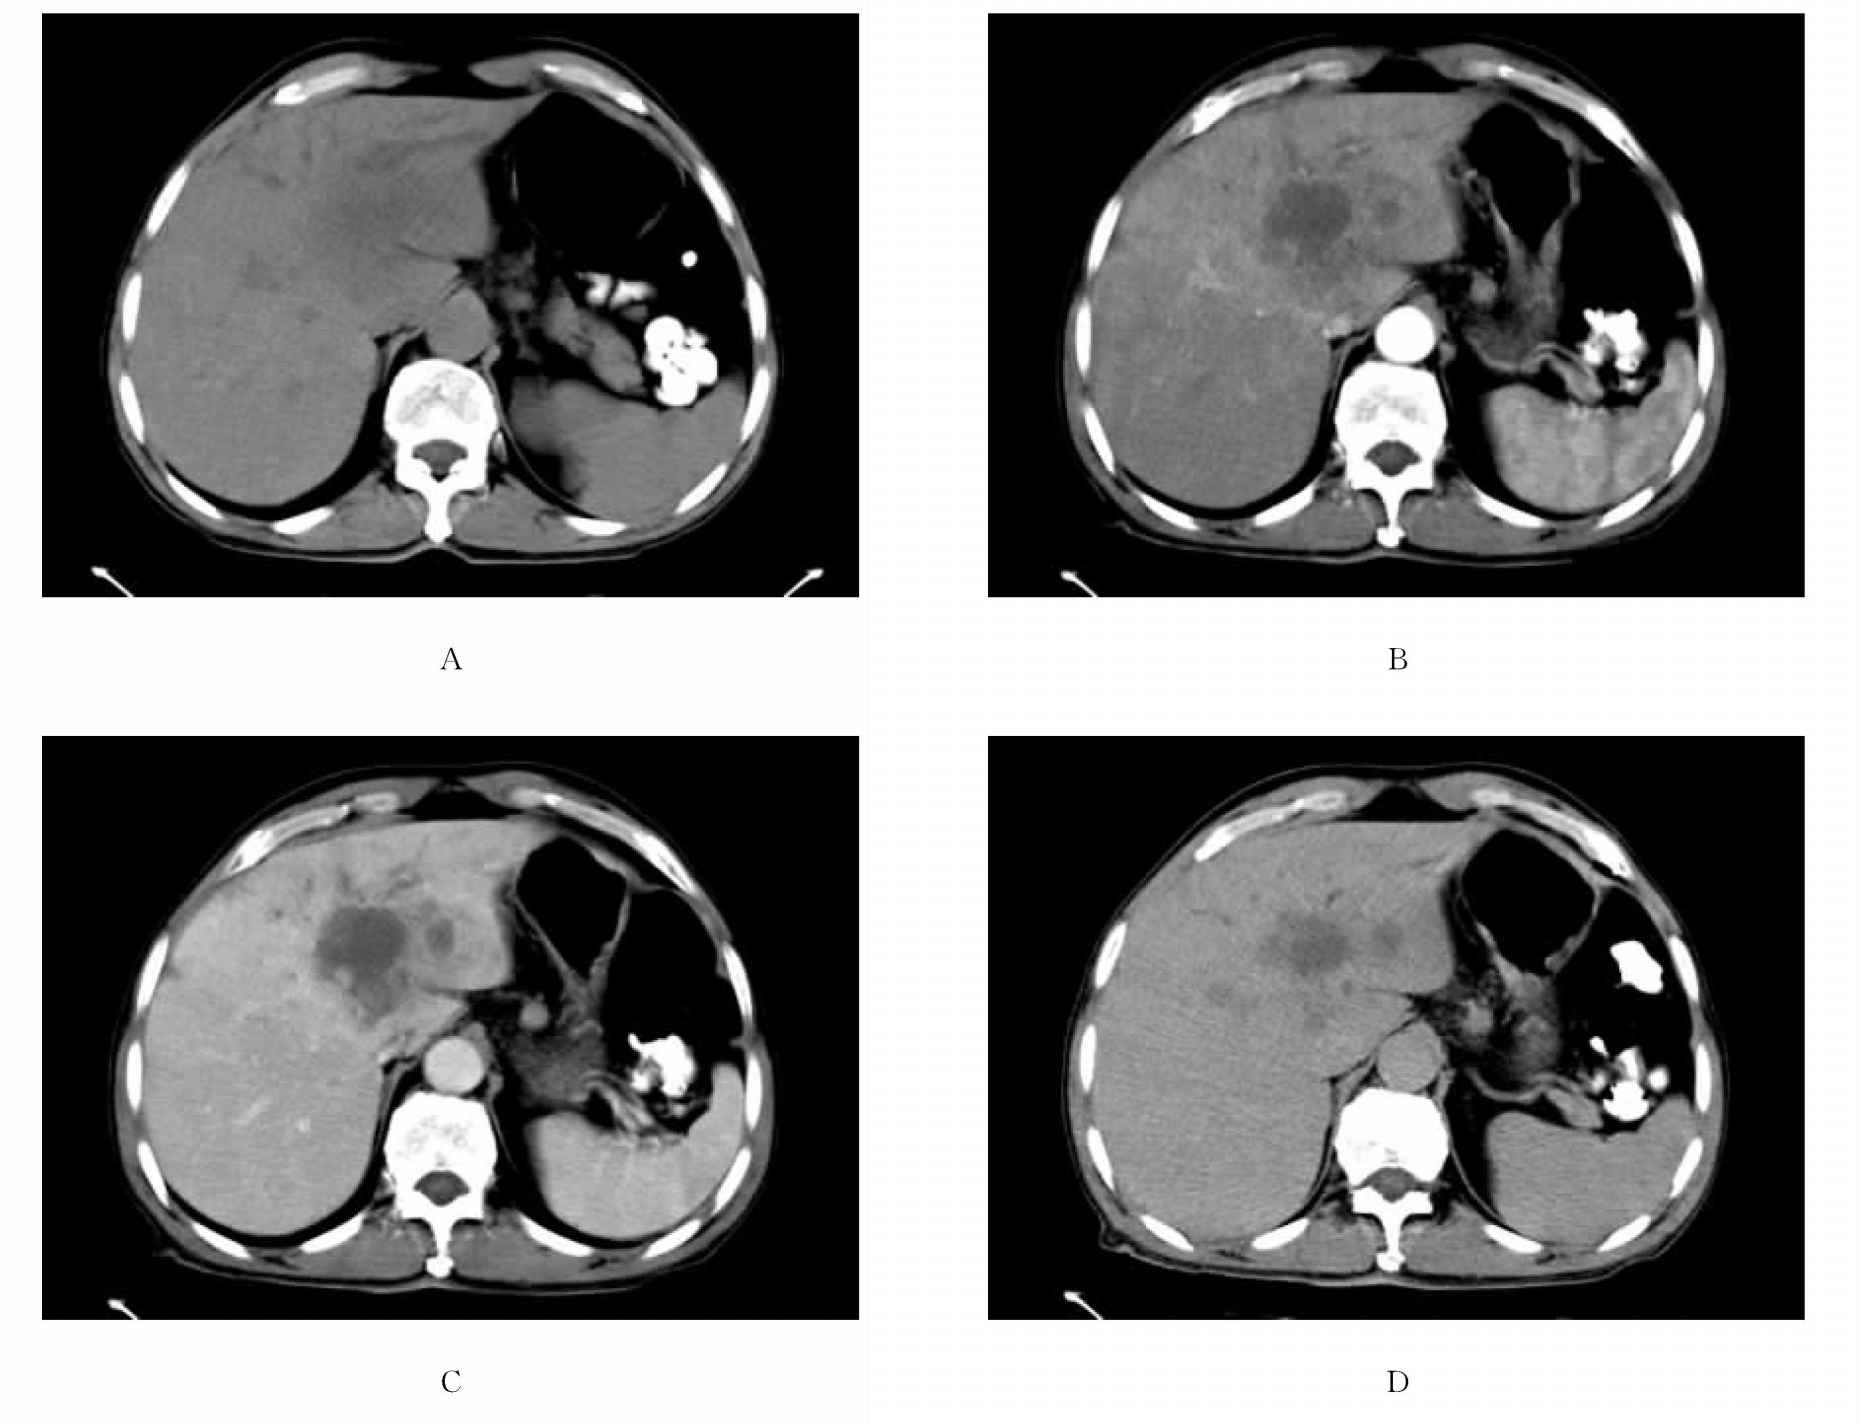
\includegraphics[width=.7\textwidth,height=\textheight,keepaspectratio]{./images/Image00275.jpg}
 \captionsetup{justification=centering}
 \caption{肝内胆管细胞癌\\{\small A~D为同一患者。A为平扫,呈边缘欠清的团块状低密度灶,邻近胆管扩张;B、C分别为动脉期和门静脉期,病灶边缘不连续的薄壁环状轻度强化,周围有卫星灶;D为延迟10min扫描,有明显向心性强化}}
 \label{fig11-4}
  \end{figure} 

总之,如病灶较大,且瘤体内有点状钙化或大片状的无强化的液性密度区出现,应考虑本病。肿瘤边缘不连续的薄壁环状轻度强化及低密度肿瘤内含有无定形的稍高密度影,是双期增强扫描的典型表现。延迟扫描可有强化及向心性强化。

\textbf{【鉴别诊断】}

1.肝内胆管细胞癌最常见的强化类型是肿瘤边缘不连续的薄壁轻度环状强化,借此即可与富血供的肝细胞癌相鉴别,结合其他表现鉴别不难。

2.肝少血供的转移瘤尤其是胃肠道来源的腺癌,CT表现可与胆管癌相似。胆管癌无原发性病灶、瘤体相对较大及伴胆管扩张有助于诊断,而且肝内胆管癌的独特表现是肝动脉期及门静脉期肿瘤呈低密度内含无定形的稍高密度影。

3.还应注意:①末梢部胆管乳头状胆管癌常以末梢胆管局限扩张为惟一表现,需注意与肝内胆管结石鉴别。②如肝内胆管癌侵及肝总管分叉区需与肝门胆管癌鉴别。③肝血管穿行在病灶中曾被认为是局灶性脂肪肝与肝占位鉴别的重要征象,但亦可见于淋巴瘤、转移性黑色素瘤、转移性腺癌以及肝内胆管癌。

\subsection{肝内胆管细胞囊腺癌}

本病比较少见,好发于中年女性。起源与胆管细胞癌一样,是具有分泌黏液功能的一种特殊类型。在病理学与胆管细胞囊腺瘤相对应,普遍认为胆管细胞囊腺瘤是囊腺癌的癌前病变。也有人认为孤立性囊肿可恶变为囊腺癌。

\textbf{【病理】}
囊壁和分隔厚薄不均,可见乳头状、结节状或扁平组织突入囊内。镜下见囊腔衬覆柱状、立方或扁平的分泌黏液细胞,可见多灶性上皮呈多层排列、特征性的乳头状结构并出现核分裂及间质内浸润。常见囊内壁被覆良性立方或扁平细胞过渡至恶性区间,囊壁可钙化。免疫组化显示其表型与胆管癌类似。

\textbf{【临床表现】}
缺乏特征性症状,常以腹部肿块为首发症状,也可有右上腹痛及间歇性黄疸、消化不良、食欲减退、恶心、呕吐等少见症状。

\textbf{【CT表现】}
平扫呈单房性或多房状囊性病变,壁较厚,并有乳头状壁结节突向腔内。囊壁大部分清晰,小部分壁厚而毛糙。常有远端肝内胆管扩张,并易造成肝内自身转移形成卫星灶。少数伴有囊壁或分隔钙化、囊内出血。综合有关文献增强扫描肿瘤实质、壁结节及纤维间隔有强化,动脉期强化较著或等于肝,门脉期、延迟期可有持续强化或无持续强化(低于肝脏)。

\textbf{【鉴别诊断】}
①与囊腺瘤十分相似,难以鉴别。但囊腺癌或囊腺瘤恶变部分的局部囊壁或间隔常较厚而毛糙、伴有粗大钙化,与周围界限不清;壁结节较多且大、实性部分相对较大及卫星灶、囊内出血等有助于鉴别。②应注意与肝囊肿、脓肿、囊性转移瘤等相鉴别。

\subsection{胆神经内分泌癌}

神经内分泌癌也称为类癌或嗜银细胞瘤,极为少见。该肿瘤一般好发于胃肠道,其次是肺脏,发生于肝脏者常为转移性,原发于肝、胆部位者罕见。

\textbf{【病理】}
神经内分泌癌一般起源于神经嵴Kulchisky细胞(嗜银细胞肿瘤),具有分泌生物活性多肽类激素和神经介质的功能。瘤细胞较小,大小均匀一致。细胞核多呈圆形,核分裂象多。胞质内具有特征性的内分泌颗粒,颗粒具有胃泌素和胰多肽的功能;成熟的颗粒所含的激素具有生物活性,不成熟的颗粒内含激素前体,生物活性低。嗜银染色(+),免疫组织化学标记中CgA是特异性较高的神经内分泌标记物,对该瘤的诊断价值很高。

\textbf{【临床表现】}
本病的术前诊断主要依赖于典型的类癌综合征即皮肤潮红、腹痛、腹泻、哮喘等症状。国内报道1组肝、胆部位者共计5例,其中4例长期腹泻(最长达1年以上),药物难以控制;其中2例腹痛。有些无典型症状者,与瘤细胞内的内分泌颗粒生物活性低或无功能有关。

\textbf{【CT表现】}

1.肝脏病变:肝内不均匀低密度肿块,大者可达30cm。瘤内常有小坏死液化区,肿瘤广泛出血坏死时则形成巨大囊实性肿块。增强扫描早期呈不均匀强化(富血供肿瘤),晚期肿瘤逐渐转变为等密度及低密度。易发生肝内转移。

2.胆囊病变:腔内隆起性病灶,无特异性征象,很难与息肉、腺瘤和腺癌鉴别。

\subsection{肝母细胞瘤}

原发性肝肿瘤占小儿腹部肿瘤的15%,2/3为恶性。肝母细胞瘤是胚胎源性恶性肿瘤,占小儿原发肝恶性肿瘤的首位(51%~56%)。

\textbf{【病理】}
由上皮和间叶两种成分组成。上皮成分又有原始肝细胞和肝癌细胞两种。间叶成分主要是骨样组织、肌肉以及髓外造血组织。大体病理可分为块状型、多结节型和弥漫型。

\textbf{【临床表现】}
好发于3岁以内的婴幼儿,以1岁以下更多见,亦可见于儿童或成年人。男女发病率之比约3∶1。常表现为厌食、体重减轻和上腹部肿块,并可出现黄疸。AFP可明显升高。

\textbf{【CT表现】}
好发于右叶,大多表现为肝内单个球形或分叶状融合的实性低密度肿块,亦可表现为多发结节(图\ref{fig11-5})。肿瘤大部分悬垂或突入腹腔,似外生型的肾母细胞瘤。肿瘤界限多较清晰,可有假性包膜;密度大多不均匀,内有放射状、裂隙状或不规则更低密度区,亦可有条索状、颗粒状等钙化表现。增强扫描可呈不均等或弧线状、网格状轻度强化,个别显著强化;其强化常延至门静脉期,考虑与肿瘤内血窦有丰富的胶原纤维分隔以及静脉参与有关;动脉期包膜有时可显著强化。很易发生肝内、外转移,最常见的部位是肺、腹部淋巴结,骨骼转移亦可见。可有肝静脉、门静脉、下腔静脉瘤栓形成。

\begin{figure}[!htbp]
 \centering
 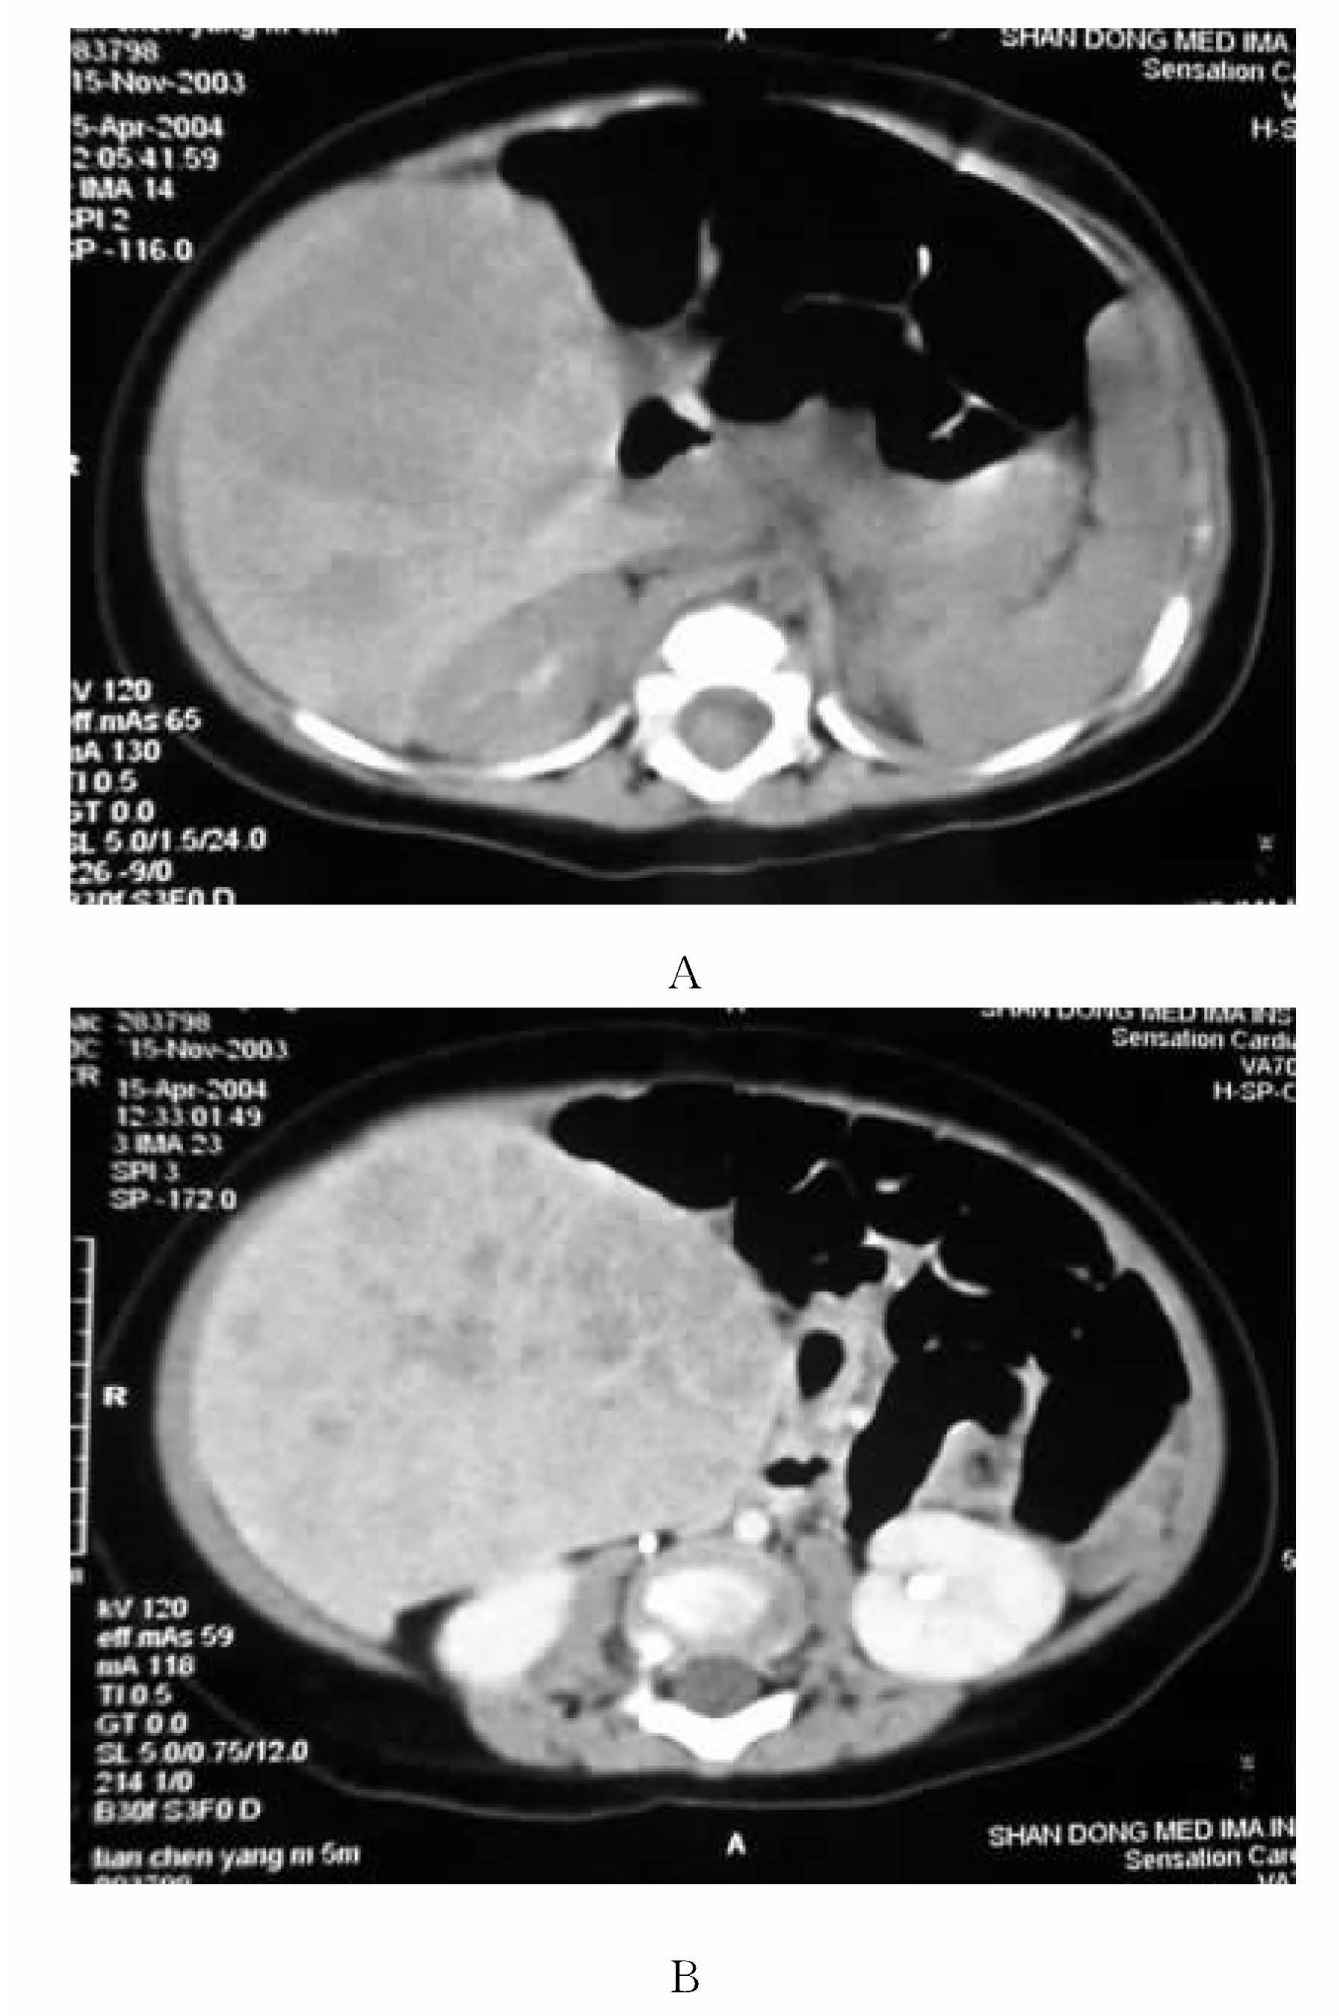
\includegraphics[width=.7\textwidth,height=\textheight,keepaspectratio]{./images/Image00276.jpg}
 \captionsetup{justification=centering}
 \caption{肝母细胞瘤\\{\small A、B为同一患者,为5个月患儿。肝右叶有巨大团块状低密度灶,密度欠均匀;病灶突向肝外,界限较清晰}}
 \label{fig11-5}
  \end{figure} 

\textbf{【鉴别诊断】}
需注意结合发病年龄、AFP与原发性肝细胞癌、横纹肌肉瘤、转移瘤(如神经母细胞瘤肝转移)、婴儿血管内皮瘤等鉴别。

\subsection{肝脏恶性间叶瘤}

本病又称为未分化胚胎性肉瘤,罕见。有人认为它是良性间叶错构瘤的恶性变。

\textbf{【病理】}
多位于右叶。剖面见大小不等的囊,内含坏死碎屑、血液、凝血块或胶样物质;部分以囊性为主或囊实各半。组织学在肿瘤的黏液性基质中含有未分化的肉瘤组织。

\textbf{【临床表现】}
多见于6~10岁儿童,多无性别差别。表现为上腹部肿块和(或)上腹痛。还可有发热、黄疸、体重下降,AFP阴性,存活期约1年。

\textbf{【CT表现】}
多为多房囊性,有不同程度的实性部分(条块状突起和囊内条索影),界限清晰,可有钙化。增强扫描假包膜可强化,肿瘤实性部分和间隔可强化,但强化常不及肝组织。

\textbf{【鉴别诊断】}
应注意与良性间叶错构瘤鉴别。后者多发生于3岁内儿童,CT表现为病灶内多数大小不等的囊,囊壁光滑,无钙化,囊内密度不一致;实性部分可较显著强化。

\subsection{肝脏横纹肌肉瘤}

\textbf{【临床表现】}
多见于5~11岁儿童。多表现为上腹部肿块和(或)上腹痛,AFP阴性。

\textbf{【CT表现】}
肿瘤呈边缘较清楚的不均匀低密度,可位于肝门区或左右肝内。出血坏死少见,罕见钙化。

\subsection{肝血管肉瘤}

本病又称为恶性血管内皮细胞瘤。

\textbf{【病因病理】}
可为先天性血管内皮瘤恶变,也可为后天发生。可能与酒精性肝硬化及接触放射性核素、氯化烯、砷化物等致癌物质有关。肉眼呈灰棕色肿块,有时如海绵窦状,经肝窦广泛侵犯肝脏。易发生出血,瘤内可见多发出血灶、凝血块与陈旧性血液相混杂之囊性变为其特征。肿瘤由各种异形的血管内皮细胞构成。

\textbf{【临床表现】}
好发于50~60岁,男性多见。患者多迅速出现黄疸、腹水,并发生肝昏迷。预后差,常早期发生肺、骨转移,并可广泛播种于腹腔。

\textbf{【CT表现】}
肝内巨大低密度病变,其内有密度不均之多种形态改变。强化方式多种多样。于动脉期可见边缘显著强化,并见内部间壁样结构,肝内转移灶也示强化。此后可见强化区向中心扩散,但不均匀,囊变区仍呈低密度。部分病例可先见病灶中心斑点样强化,而无边缘强化。弥漫侵犯时,可见肝脏体积增大,肝内多发弥漫性病变,并有不规则强化。

\textbf{【鉴别诊断】}
本病与海绵状血管瘤表现类似,但本病内部结构复杂如有许多囊变区,且常为多发病变、弥漫性侵及全肝等,与血管瘤典型表现为进行性向心性结节状强化有别。

\subsection{肝脏上皮样血管内皮瘤}

本病亦称为组织细胞样血管瘤,是一种极为罕见的血管源性恶性肿瘤,临床过程介于血管瘤和血管肉瘤之间,也有学者将其视为血管肉瘤的一种罕见类型。其病因不明,主要见于成年女性,可能与口服避孕药有关。

\textbf{【病理】}
组织学上肿瘤由树枝状和上皮样细胞构成,常包含代表细胞内腔的空泡,基质由纤维构成,有玻璃样变区域。免疫组化至少对一种内皮标记物即因子Ⅷ相关抗原、CD34和(或)CD31呈阳性,尤以细胞中含因子Ⅷ相关抗原是诊断的关键。肿瘤外周为富细胞区,中心为富含纤维的硬化区。

\textbf{【临床表现】}
无特异性,上腹部隐痛、不适为常见症状。还可表现乏力、体重减轻、食欲减退、黄疸等症状。

\textbf{【CT表现】}
肿瘤较多的位于肝脏周边区域,肝包膜无膨隆,甚至内缩(由于肿瘤的纤维基质成分可在肝实质中产生一种纤维收缩反应所致)。常为多发。平扫呈不均匀低密度,中央可有更低密度区,部分可有钙化。增强扫描表现为类似于血管瘤的“早出晚归”和向心性强化模式,但其强化表现为怪异形状的非结节状,且强化程度均低于同期的腹主动脉和门静脉,中央区常有索片状无强化区;小结节灶多呈周边环形强化。

此病预后较血管肉瘤好,不足30%发生肝外转移,应注意鉴别。

\subsection{恶性血管外皮细胞瘤}

血管外皮细胞瘤是少见的血管肿瘤,发生率不及全部血管瘤的1%。可发生于任何年龄、任何部位,但多见于四肢、躯干、盆腔、腹膜后,肝脏少见。

\textbf{【病理】}
其组织学来源为血管外皮Zimmermann氏细胞,近年来有学者认为其来源为血管外周多功能间质细胞。病变多为单发,偶为多发,大小从数毫米至数厘米。病理单纯依靠光镜较难判断其生物学行为,但有丝分裂增多,细胞退行性变明显提示恶性程度较大。由于肿瘤良恶性之间无明显可靠的组织学鉴别标准,所以有人认为所有肝血管外皮细胞瘤应考虑或视为潜在恶性肿瘤。

\textbf{【临床表现】}
本病好发于20~70岁,男性略多。一般表现为肝脏无痛性肿块。

\textbf{【CT表现】}
①病变<3.0cm时,多为实性,无包膜,少有囊变坏死,故平扫时呈密度均匀的低密度灶。因血供丰富增强扫描于动脉期显著均匀强化。②3.0~5.0cm的肿瘤,平扫时呈均匀的低密度。增强后自周边向中心逐渐强化,类似血管瘤表现。③当病变较大时,常有完整的包膜形成,其中心区可有出血、坏死和囊变,故平扫呈混杂密度。增强早期包膜或周边环状强化,但延迟后呈混杂密度,囊变区不强化,类似巨块型肝癌。

\textbf{【鉴别诊断】}
①海绵状血管瘤:血管外皮细胞瘤于动脉期的强化程度低于血管瘤,于静脉期一般呈等密度,稍大者呈环状强化,但无血管瘤之边缘结节样强化并迅速向中心推进的特点。②小肝癌:动脉期呈明显均匀的强化,但门静脉期迅速变为低密度,且多有完整包膜,有助于和血管外皮细胞瘤鉴别。③巨块型肝癌:血管外皮细胞瘤呈中等密度的边缘强化,强化程度高于肝癌、低于血管瘤并有向中心推进的特点,有助于和肝癌鉴别。

\subsection{肝脏恶性纤维组织细胞瘤}

恶性纤维组织细胞瘤四肢多见,其次是腹膜后、腹膜腔和躯干等,肝脏罕见。

\textbf{【病理】}
恶性纤维组织细胞瘤为具有纤维细胞形态的细胞与具有组织细胞某些形态及功能特征的细胞彼此混合的肿瘤,属肉瘤性质。其组织学来源尚无定论,可能来自组织细胞或原始间叶细胞。发生于肝脏者其组织学特点与发生于软组织者相似,也可分为4个亚型:①席纹状多形性型;②黏液型;③巨细胞型;④炎症型。

\textbf{【临床表现】}
该病可发生于任何年龄,以老年人多见,男多于女。临床与肝癌和肝脓肿相似。主要表现为肝区疼痛、发热及消瘦,部分病人出现厌食、全身不适等。晚期偶见外周WBC异常增多。

\textbf{【CT表现】}
其表现无特异性。主要表现为形态不规则的低密度占位。肿瘤向周围浸润明显而致边界模糊不清,容易侵犯肝包膜和邻近组织。肿瘤中心坏死显著,实质部分所占比例很小,内缘毛糙。瘤内出血常见。增强扫描肿瘤周边的实质部分逐渐强化,即动脉期轻度强化,门静脉期中度强化。

\subsection{肝脏Kaposi肉瘤}

本病又称特发性多发性出血性肉瘤。

Kaposi肉瘤腹内实质性脏器受累主要有肝脏、胰腺和肾上腺。在腹部还可累及腹膜后间隙、肠系膜、盆腔(包括直肠及直肠周围间隙)。

\textbf{【CT表现】}
平扫见肝内小的低密度灶,肝门及肝实质内门脉分支影不规则扩大。增强扫描示门静脉分支旁肝实质内多个散在的低密度影,比平扫时显示更多;4~7min后延迟扫描大部分强化并与肝实质密度相近或稍高,但其病理基础尚不明确。

\subsection{肝脏肉瘤}

本病是起源于肝脏间叶组织的恶性肿瘤,罕见,以血管肉瘤相对较多(见上述)。此外,还有纤维肉瘤、平滑肌肉瘤、脂肪肉瘤和多种成分的混合肉瘤等,而癌肉瘤更为罕见。

\textbf{【临床表现】}
常无明显症状,往往在病灶较大时以上腹部包块而就诊。实验室检查如AFP等均正常。

\textbf{【CT表现】}
①多种成分的间叶源性肉瘤:由于含脂肪和软组织成分,病灶边缘清楚。增强后软组织部分显著强化,且可显示动静脉瘘。②脂肪肉瘤:往往较大,部分病例以脂肪密度为主。但与脂肪瘤不同,内见较多纤维条索影,且有较明显增强。③其他类型的肉瘤如平滑肌肉瘤,多表现为肝内巨大低密度灶。易坏死囊变,壁厚且不规则,呈厚壁囊样或囊实性占位表现,且边缘增强明显。④癌肉瘤与HCC表现基本一致。

\subsection{肝脏恶性淋巴瘤}

本病分为原发和继发两种。

\textbf{【病理】}
原发性极为罕见,属非霍奇金淋巴瘤。继发性为全身淋巴瘤累及肝脏,脾脏多同时受累。原发性肿块呈单发或多发,无明显包膜,极少呈弥漫性浸润。继发性多呈弥漫性浸润,仅由显微镜检出或呈粟粒性、结节状或肿块。

\textbf{【临床表现】}
全身症状有发热、盗汗、原因不明的体重下降、乏力、贫血、血沉快等。肝脏增大或触及局部肿块,常伴脾脏增大。肝区可有胀痛。

\textbf{【CT表现】}

1.原发性:平扫呈单发或多发的边缘清楚、形态不规则的低密度灶,其内可有更低密度区,病灶内无钙化。增强后病灶可有不同程度的强化,但多低于肝实质。我们遇见1例延迟期呈稍高于肝实质的均匀强化。

2.继发性:往往肝、脾同时受累。平扫表现肝脏弥漫性增大,密度可无明显异常。增强后肝、脾实质均匀性强化,门脉受压变细或显示不清;也可表现为肝内弥漫分布的低密度结节或肿块,病灶边缘轻度强化。可同时显示腹腔内增大的淋巴结。

\subsection{肝转移瘤}

\textbf{【来源途径】}
主要有:①血行转移:可为门静脉性及动脉性转移;②邻近脏器直接浸润;③经肝门部淋巴性转移;④经腹膜种植。其中主要为血行转移。

原发癌主要为消化系统肿瘤、乳腺癌、肺癌等,其中来自胃、胰腺、结肠等门静脉系脏器者约占半数。另外,肾、肾上腺肿瘤也可经肝静脉产生逆行性肝转移。

\textbf{【血供】}
肝转移瘤主要由肝动脉供血、门静脉参与供血,并有人认为瘤体边缘的血供可能来自门静脉。富血供的转移灶在动脉期和门脉期均表现为环状显著强化(少数亦可发生弥漫性强化),也反映了富血供转移灶不仅接受双重供血,而且其门静脉血供主要位于肿瘤边缘的特点。

大多数转移瘤是少血供的,约4%~7%血供丰富。富血供者主要见于肉瘤、胰岛细胞瘤、肾癌、乳腺癌、类癌、胃肠道来源的黏液腺癌、黑色素瘤等。

\textbf{【病理】}
肿瘤界限清楚,中心多发生坏死、退变。可分为多发结节型、结节相互融合的块状型和境界不清的弥漫型。病灶小者仅数毫米,大者达10cm以上;单发或多发,局限或散在分布。肿瘤内部出现钙化并不少见。

\textbf{【临床表现】}
兼有原发癌症状及转移癌本身症状,一般先有原发癌症状,晚期才出现转移癌症状。少数原发癌症状不明显,而以转移癌症状为主诉。可有乏力、消瘦、肝区痛,继而为肝大、黄疸、腹水、发热等。约95%AFP阴性,少数来自胃、胰和卵巢癌的肝转移AFP可轻度升高。血ALP、LDH、GPT升高。此外,胃肠道肿瘤癌胚抗原(CEA)可升高。

\textbf{【CT表现】}
肝转移灶的大小、数目和形态表现不一。病灶越多,大小和分布越趋向均匀,直径一般在1~3cm。绝大多数呈圆形,个别大的病灶可不规则或呈分叶的巨块状。病灶一般无包膜。

\subsubsection{平扫表现}

表现为多发性大小较一致的低密度结节,也可为单发结节或巨块(图\ref{fig11-6}A)。多在低密度灶内存在更低密度区域,从而呈同心圆状或等高线状双重轮廓为其特征。如合并脂肪肝,病灶可等于或高于肝实质。肿瘤内如有新鲜出血或钙化时,其内出现高密度灶。

易出现钙化的转移瘤有:结肠黏液癌、胃黏液癌、卵巢癌、乳腺胶质癌,其他尚有胰岛细胞瘤、平滑肌肉瘤、黑色素瘤和骨肉瘤等。

\subsubsection{增强扫描}

其增强表现主要取决于肿瘤本身的血供。有学者认为转移瘤的边缘强化,可能与肿瘤边缘结缔组织、炎性细胞浸润和血管增生有关。

1.病灶边缘强化:因血供程度不一,而强化程度不一,如血供丰富的肉瘤等可高于肝组织(图\ref{fig11-6}B),但大多低于周围肝实质。病灶中央因坏死、囊变而更低,肿瘤体积较大或肉瘤转移灶容易出现坏死和囊性变。还有的原发肿瘤本身为囊性结构如卵巢、胰腺的囊腺癌,转移到肝脏后仍呈囊性表现,甚至呈其典型的原发癌特征。

\begin{figure}[!htbp]
 \centering
 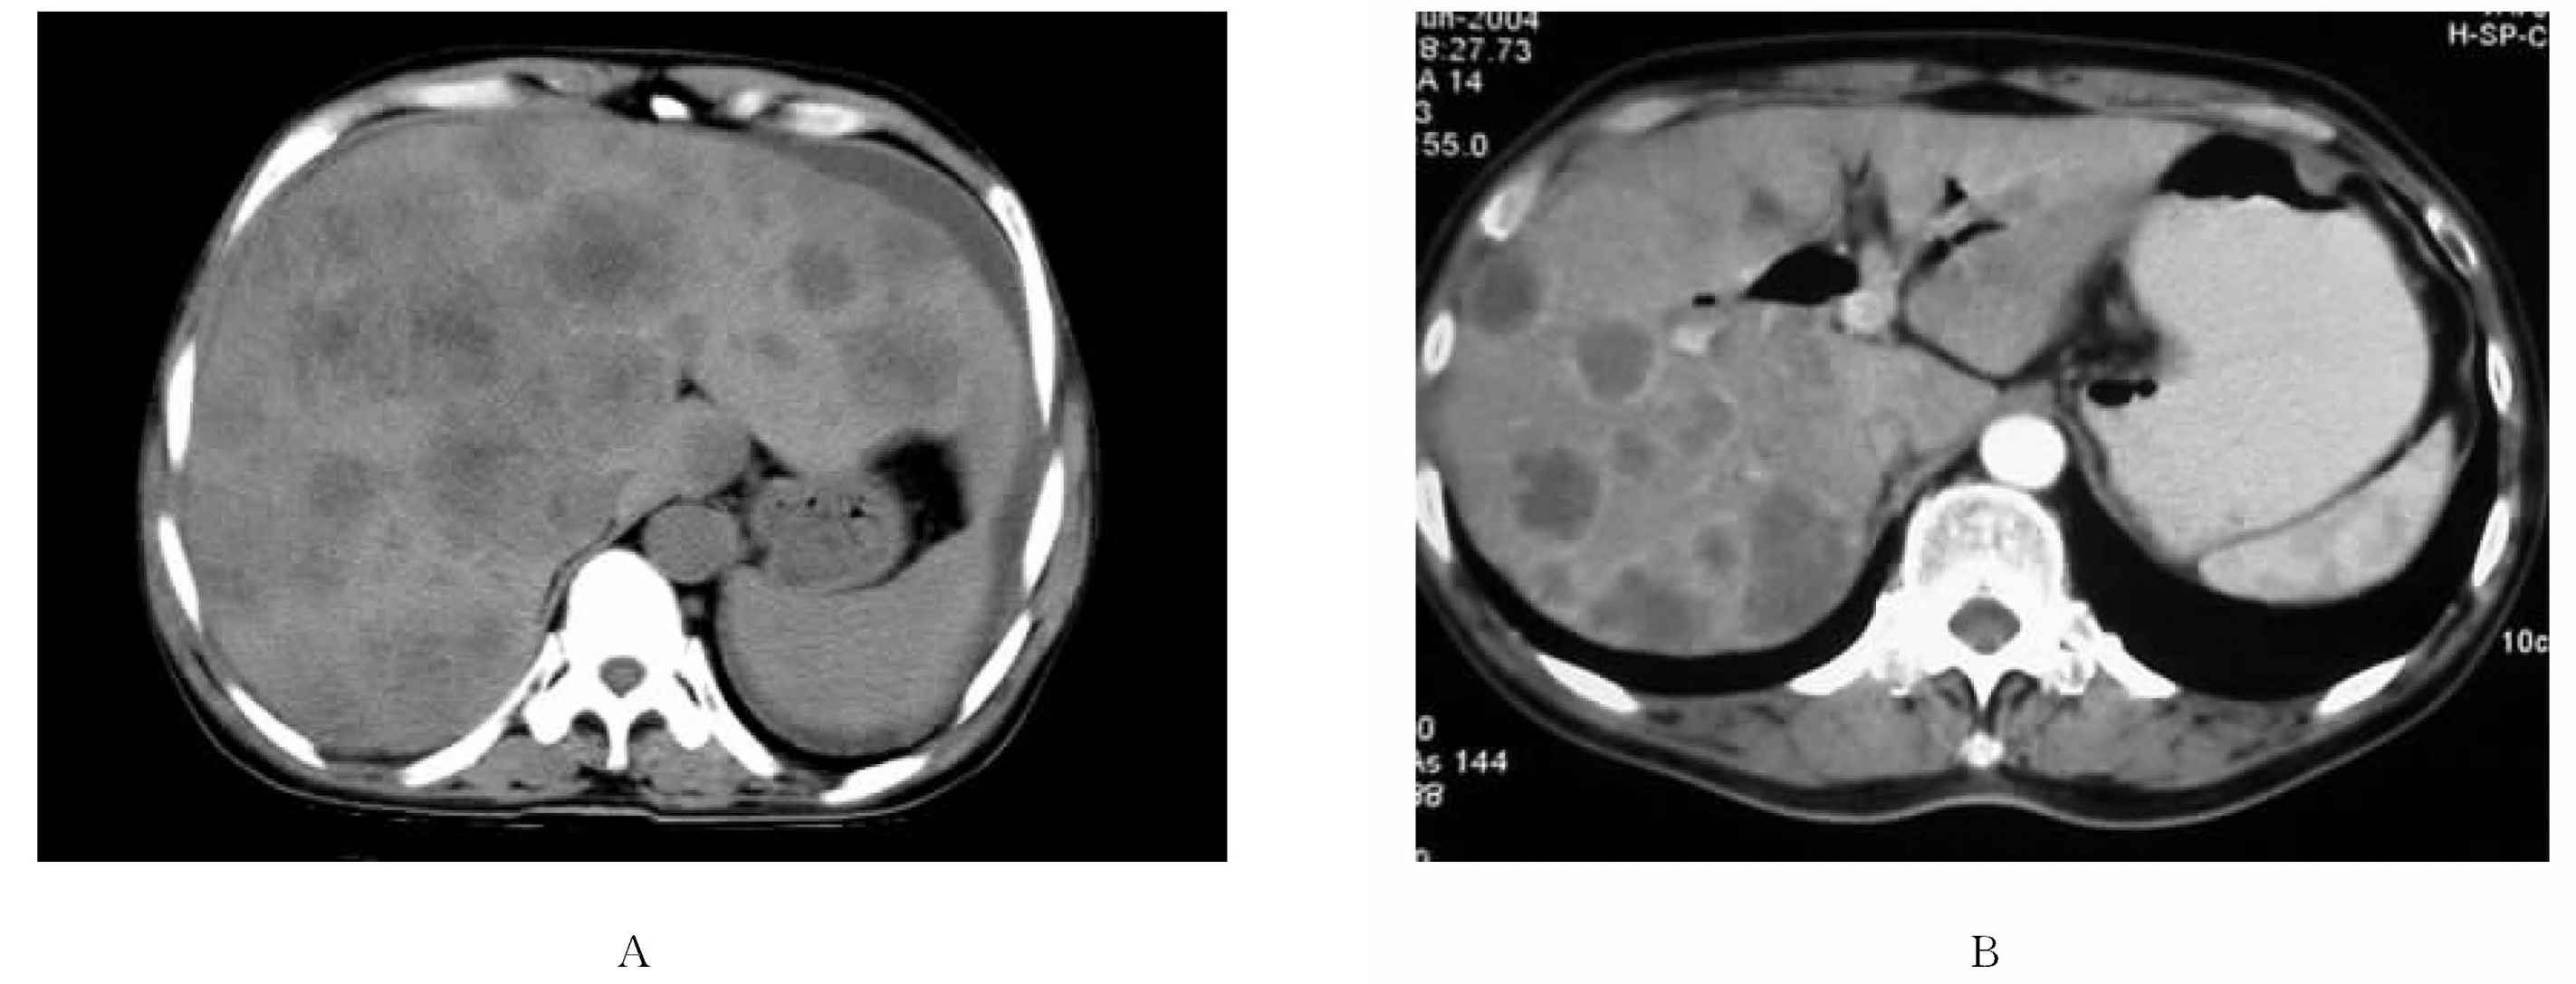
\includegraphics[width=.7\textwidth,height=\textheight,keepaspectratio]{./images/Image00277.jpg}
 \captionsetup{justification=centering}
 \caption{肝转移瘤\\{\small A、B非同一患者。A为平扫,肝左右内弥漫性分布有许多低密度结节,肝脾周围有腹水;B为增强扫描动脉期,病灶边缘强化}}
 \label{fig11-6}
  \end{figure} 

2.肝转移瘤可有灶内结节样强化或团块状强化的表现,并认为可能是正常肝组织对比剂浓度下降和病灶本身强化的结果。有文献报道以大肠癌、胃癌、乳腺癌为代表的腺癌肝转移,由于肿瘤周边部分被存活的瘤细胞所占据,中心被纤维组织和坏死组织随占据,故增强扫描早期为边缘增强,中心为低密度;10分钟后延迟扫描边缘为低密度,中心为高密度为其特征(这一特征与肝内胆管癌相似)。也可出现边缘强化及向心性强化的特点(图\ref{fig11-7})。国内还有学者报道1组全身化疗后的肝转移瘤呈“类血管瘤样强化”。

3.整个病灶均匀或不均匀强化,通常低于周围肝组织。

\begin{figure}[!htbp]
 \centering
 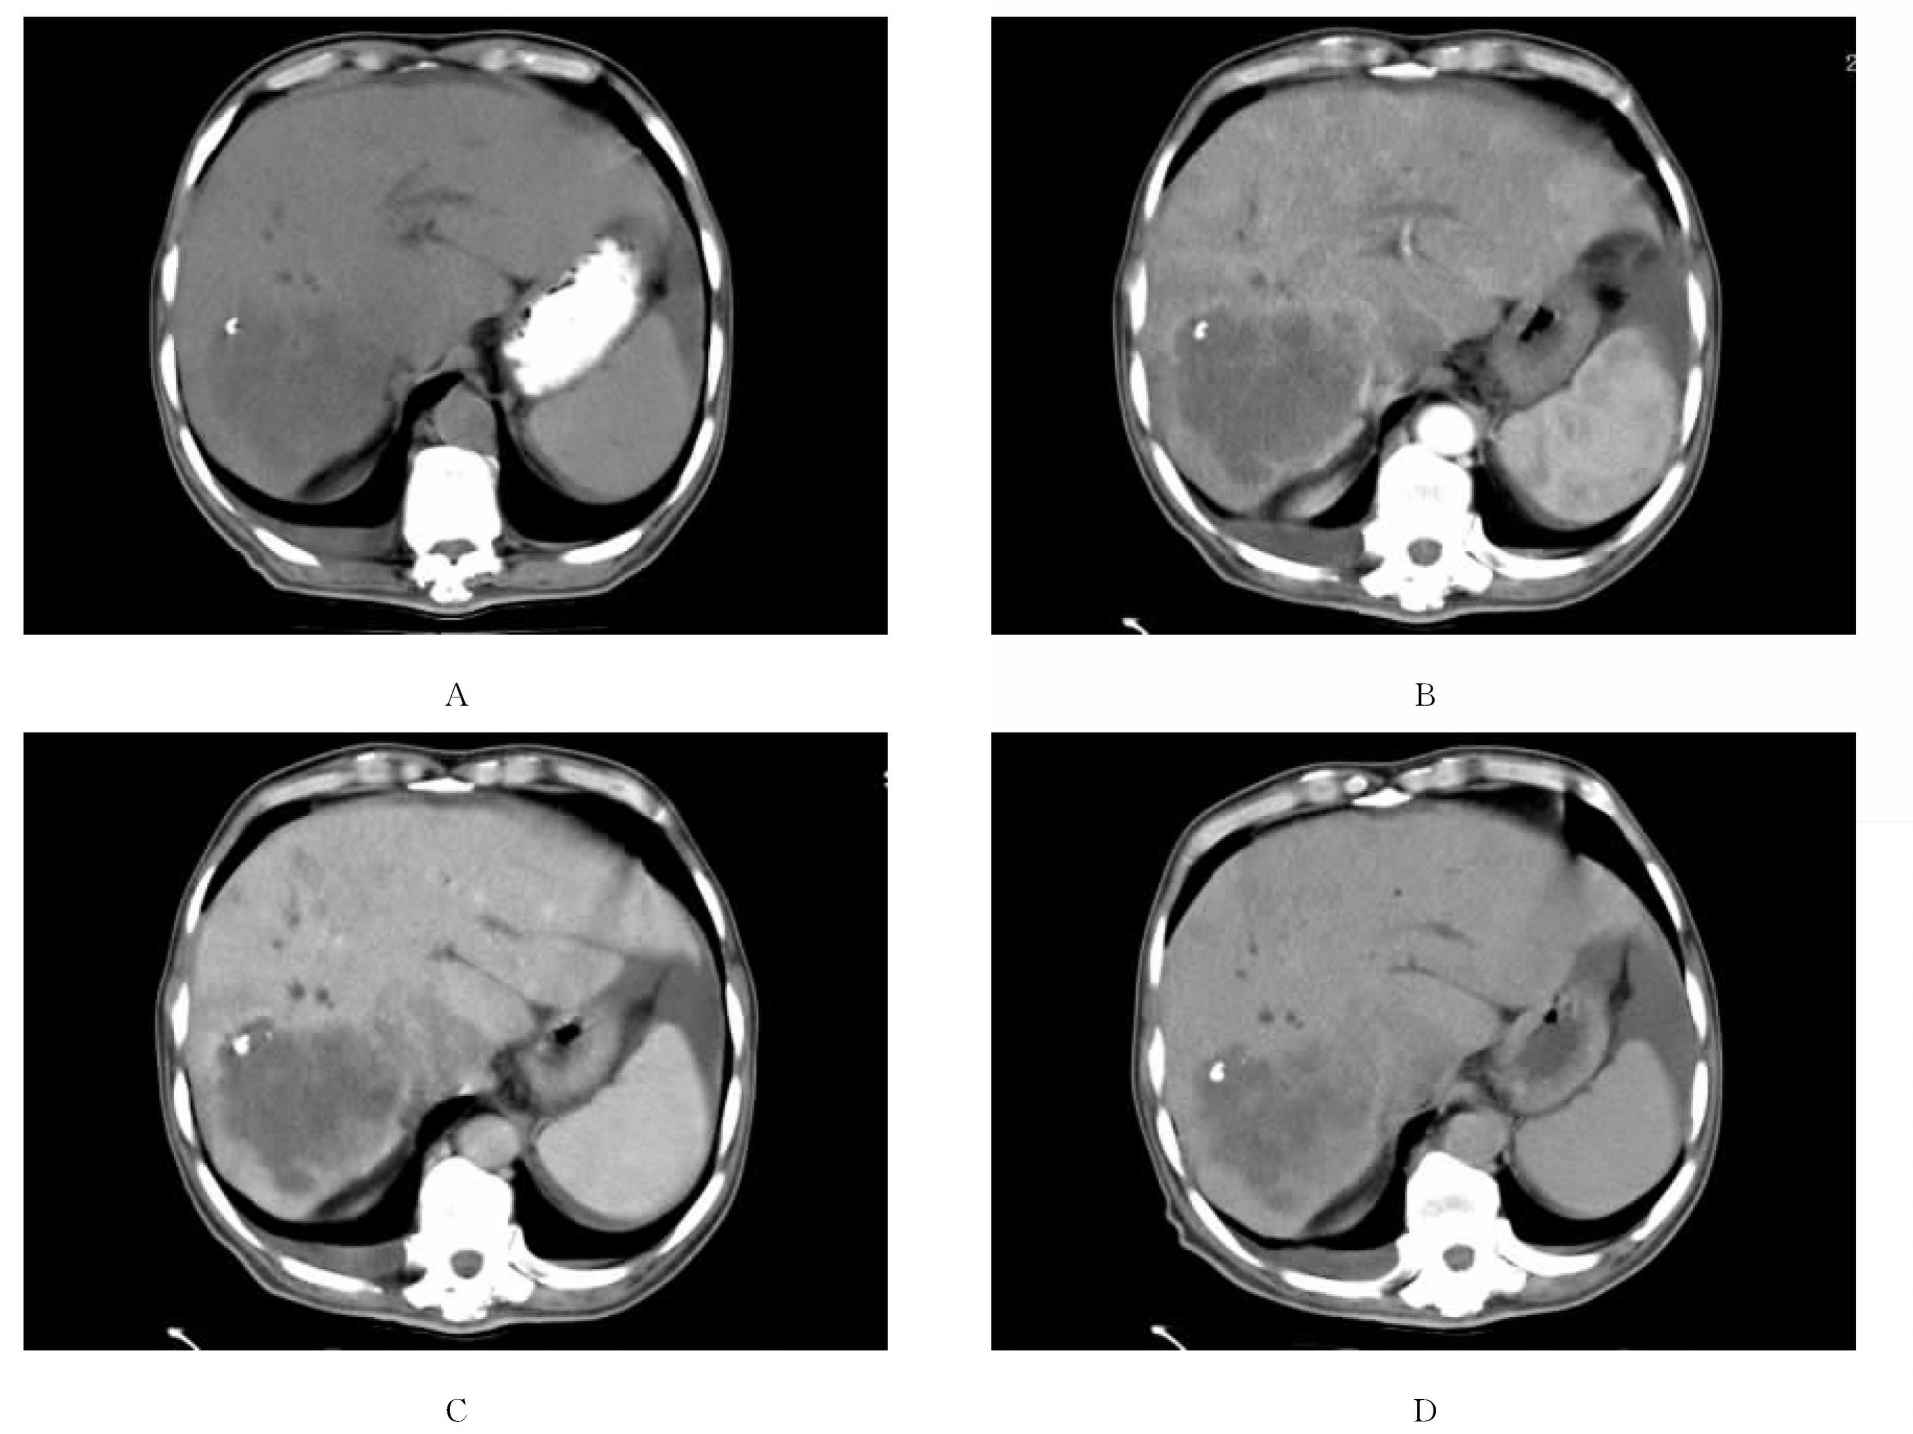
\includegraphics[width=.7\textwidth,height=\textheight,keepaspectratio]{./images/Image00278.jpg}
 \captionsetup{justification=centering}
 \caption{肝转移瘤(巨块状)\\{\small A~D为同一患者。A为平扫,B为动脉期,C为门静脉期,D为延迟7min扫描;显示动脉期和门静脉期病灶边缘稍强化,延迟扫描有向心性强化趋势}}
 \label{fig11-7}
  \end{figure} 

4.富血供的转移瘤可以与肝实质一样迅速增强,其密度与肝实质相同,而致增强扫描反而不如平扫时明确。

5.转移瘤尤其大的病灶,可因坏死液化而呈囊样改变,强化后更著,少数瘤壁很薄且光滑类似囊肿。小的转移灶也可发生坏死。

6.“牛眼征”即病灶中心为坏死液化的低密度,边缘强化,再向外的最外层密度又低于肝实质。也有中心为高密度的。一般认为该征多见于平滑肌肉瘤、恶性神经鞘瘤和其他肉瘤转移等。

此外,大的转移灶可侵犯局部血管,但较少见到癌栓形成;病灶亦较少见到代表假包膜的“晕圈征”。

\textbf{【鉴别诊断】}
根据临床并结合下列CT征象不难与其他疾病相鉴别。支持转移瘤的CT征象为:病灶多发、散在和大小相仿;明显边缘增强和“牛眼征”,较小病灶出现囊样变伴边缘强化;无门脉癌栓和周围晕圈;邻近原发肿瘤、复发灶和转移灶。但是增强扫描转移瘤、肝脓肿、胆管细胞癌、血管瘤均可出现边缘强化及向心性强化的特点,尤其单发转移瘤可与不典型肝脓肿、胆管细胞癌鉴别困难(如图\ref{fig11-7})。

1.原发性肝癌:单个或数目不多的转移灶与原发肝癌鉴别有一定困难。①大小不一,特别表现为大病灶周围有结节灶(卫星灶)者,以原发性肝癌可能大。②原发性肝癌呈速升速降的强化特点有别于转移瘤。③病灶周围的晕圈征和门脉癌栓形成,明显支持原发性肝癌。④小瘤内囊样变一般不见于原发性肝癌,而转移瘤常见。

2.血管瘤:①两者均可出现边缘强化及向心性强化特征,但血管瘤边缘呈结节状与腹主动脉相近的强化,并向中心迅速推进有别于转移瘤。②动脉期均一强化的小血管瘤与转移瘤难以鉴别,但血管瘤在门脉期仍维持强化,富血供的转移灶则趋于消失,可资鉴别。③血管瘤更多见对比剂完全填充病灶。

3.肝脓肿:除边缘强化外,外层有低密度水肿带,与转移瘤的“牛眼征”类似,但结合转移瘤其他典型表现并结合临床不难鉴别。

4.胆管细胞癌:肿瘤边缘不连续的薄壁环状轻度强化及低密度肿瘤内含有无定形的稍高密度影,是其双期增强扫描的典型表现。

此外,极个别的囊性转移灶与肝囊肿鉴别困难,应予注意。

\subsection{肝脏囊性恶性肿瘤的鉴别诊断}

1.囊性转移瘤:远较其他的肝囊性恶性肿瘤常见。其表现多样化,以多发囊性或伴实性病灶为其特点。根据囊壁情况可分为:①薄壁型:壁厚≤3mm,壁薄而均匀;②边缘结节型:多个壁结节突入囊内;③混合型:即薄壁、厚壁或囊实性病灶并存。除薄壁型强化不著外,其他均有强化。

2.囊性肝癌:表现为单发不均或均匀厚壁型肿块,有壁结节、囊壁有强化。

3.囊性肝肉瘤:为单房或多房囊性肿瘤,囊壁及分隔多有明显强化。

4.囊腺癌或囊腺癌肉瘤:为多房囊性病变,或以多房为主的囊实性肿块,有壁结节,周围可有卫星灶及远端胆管扩张。囊壁分隔、壁结节及肿瘤实质部分均有轻度或明显强化。

5.囊性胆管细胞癌:为囊实性病变,囊性部分多呈较小、多发的囊性病灶,伴病灶远端胆管明显扩张。增强扫描肿瘤边缘不连续的环状强化及低密度肿瘤内含有无定形的稍高密度影,是其双期扫描的典型表现。可有延迟强化及一定的向心性强化表现。

6.Caroli病癌变:癌变后的特征为扩张的胆管伴管壁软组织肿块。

\section{肝血管瘤和其他良性占位性病变}

\subsection{肝血管瘤}

本病通常为海绵状血管瘤,为肝脏最常见的良性肿瘤,占肝良性肿瘤的84%。尸检发现率约为7.3%。

\textbf{【病理】}
肿瘤大小不一,小者1cm左右,大者直径超过10cm,单发多见(90%)。外观呈紫红色,一般无包膜。切面呈囊状或筛状空隙,犹如海绵,故称为海绵状血管瘤。有的中央可见瘢痕,偶见钙化。镜下见大小不等的血管腔,衬以扁平内皮细胞,管腔间被纤维组织和基质充填。根据血管腔管壁厚薄不同分为厚壁型和薄壁型两种,前者少见,因管腔小,造影剂不易进入。

\textbf{【临床表现】}
可见于任何年龄,以30~60岁多见,女性居多。可无任何症状,只有少数大者因压迫肝组织或邻近脏器产生上腹部不适、胀痛,或触及肿块,但全身情况良好。

\textbf{【CT表现】}

1.平扫:呈圆形或卵圆形低密度,界限清楚,密度均匀(图\ref{fig11-8}A);大的血管瘤有时可见中央更低密度的瘢痕,呈裂隙状、星状或不规则形,偶有钙化。

2.增强扫描:动脉期早期可见病灶边缘呈结节状、棉球状、斑点状、C字形粗线条状所组成的环状强化,其密度明显高于肝实质,与同层面腹主动脉密度相近,具有特征性。早期边缘强化的峰值出现时间约在30~60秒,较肝癌稍迟,且峰值持续时间长即高于周围肝实质密度的持续时间超过2分钟。以后造影剂从周边部向中心部扩散,呈现向中心的乳头状突出的充填征象。多于5~10分钟以后中心部完全充填,有的长达20~60分钟,致使肿瘤与周围肝实质呈等密度。当肿瘤内部有血栓或纤维化时,此部分不被充填,而仍呈低密度区域。

总之,动脉早期病灶边缘呈高密度强化,强化区域进行性向病灶中央扩散,延迟扫描病灶呈等密度充填,即所谓“早出晚归”是其特征性CT表现(图\ref{fig11-8}B~D)。

\begin{figure}[!htbp]
 \centering
 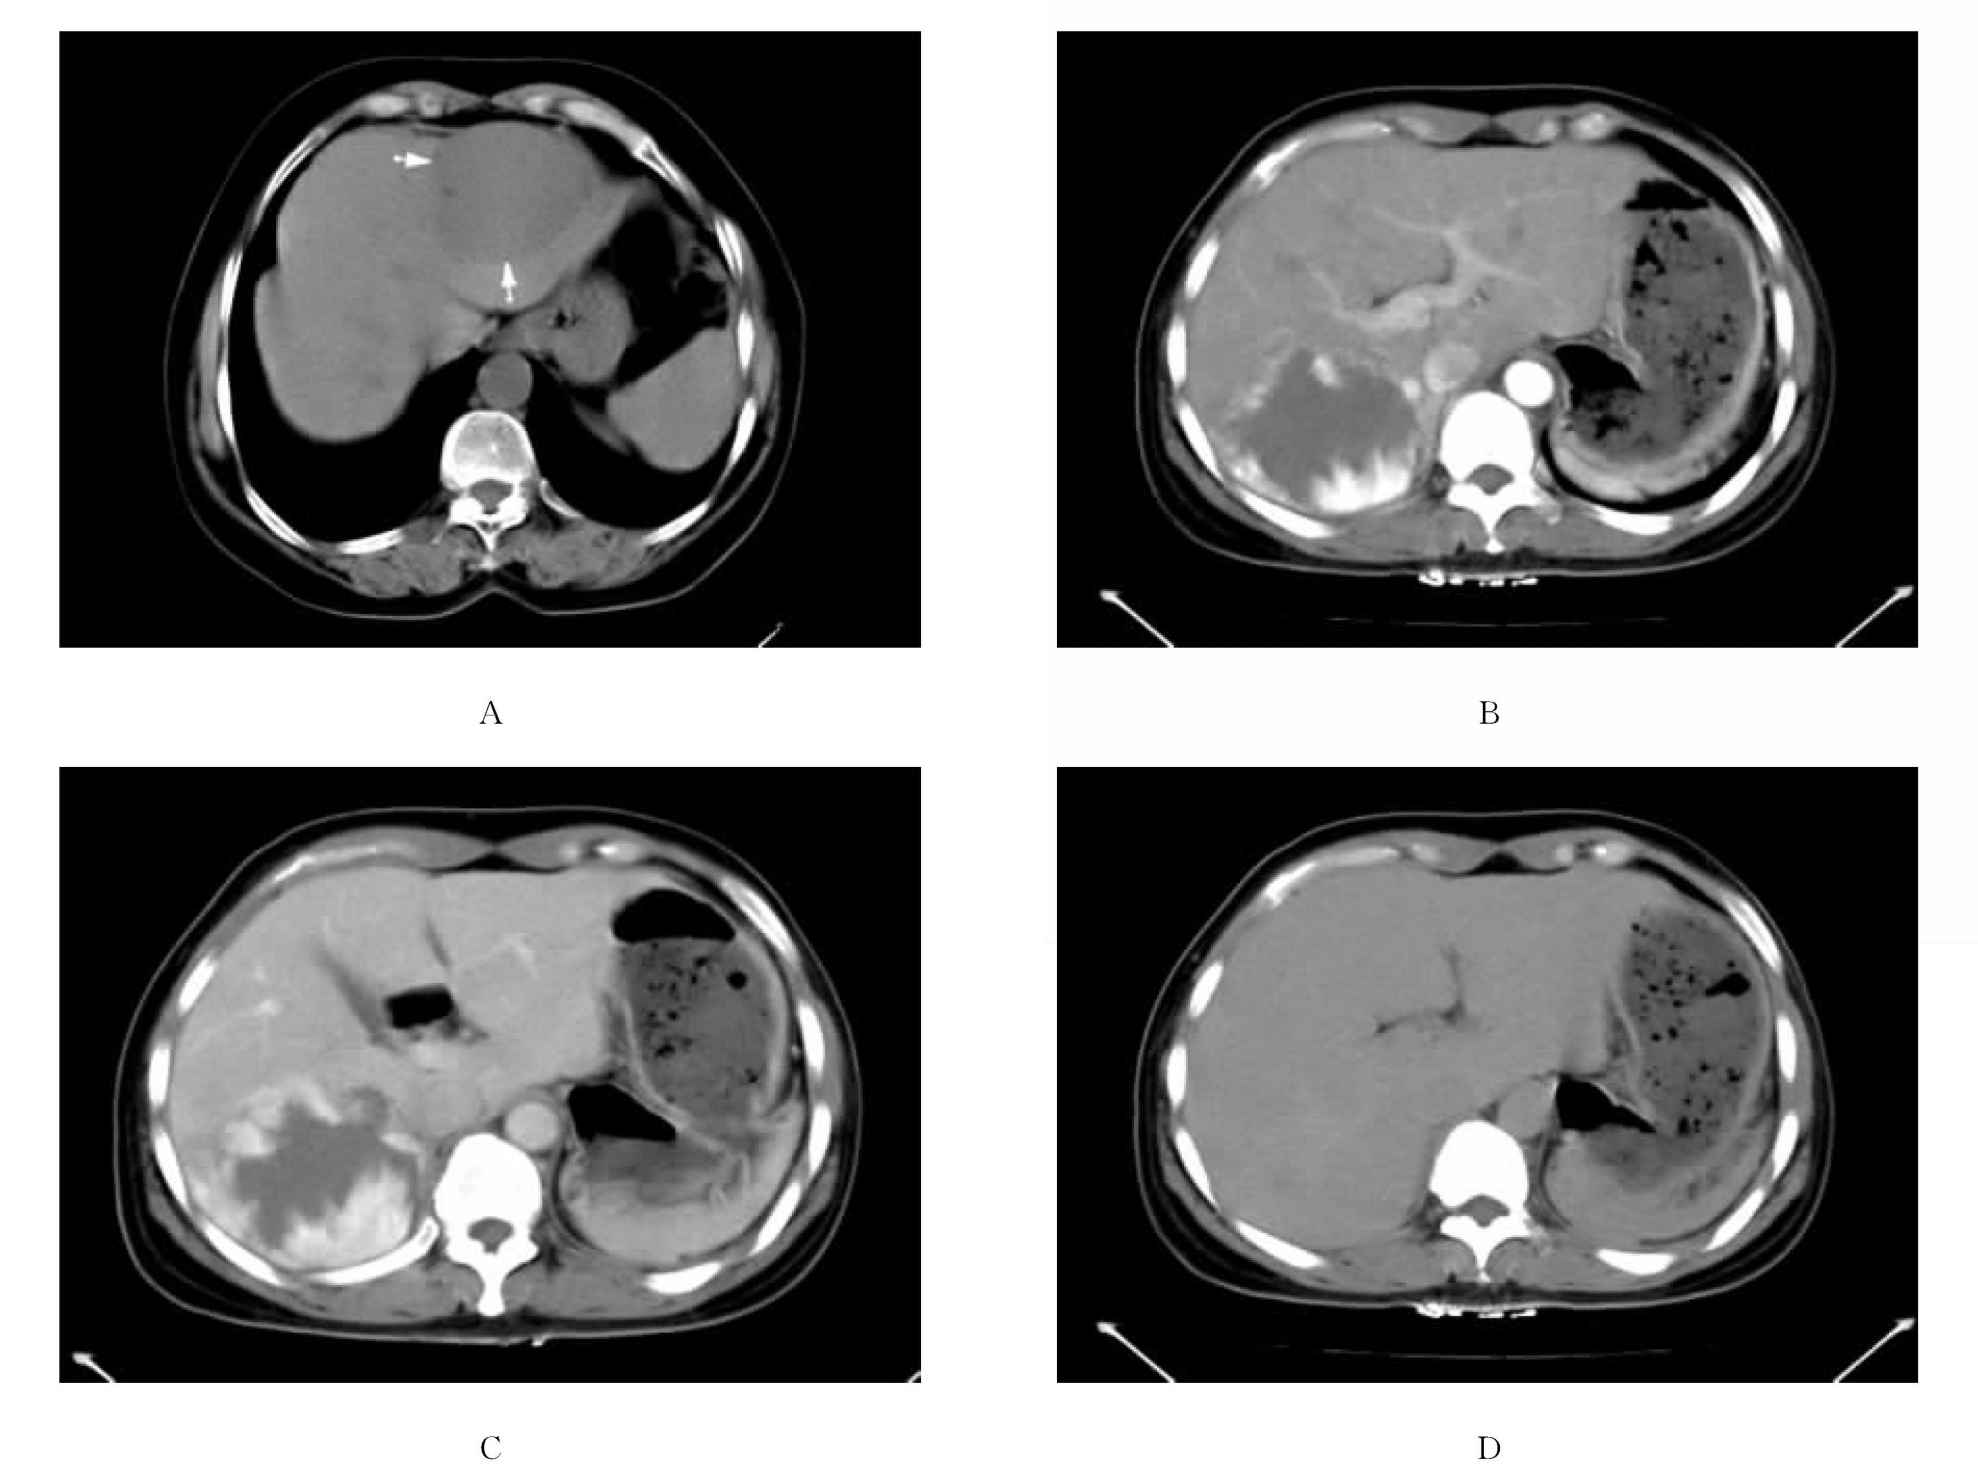
\includegraphics[width=.7\textwidth,height=\textheight,keepaspectratio]{./images/Image00279.jpg}
 \captionsetup{justification=centering}
 \caption{肝血管瘤\\{\small A示肝左叶有近圆形低密度,界限清楚,密度均匀。B~D为同一患者;B为动脉期病灶边缘呈棉球状、结节状、线条状高密度强化(与腹主动脉密度相近);C为门静脉期造影剂从周边部向中心部扩散;D为延迟11分钟扫描中心部完全充填,肿瘤与肝脏呈等密度}}
 \label{fig11-8}
  \end{figure} 

3.不典型表现:除上述典型表现外,还可见以下不典型表现。①首先在肿瘤的一部分强化,并逐渐向中心扩散,至整个病灶等密度充填。②其次在肿瘤内部呈斑点状高密度强化,其密度与主动脉接近,然后逐渐扩大、融合,至等密度充填。③肿瘤呈多数大小不等、比较密集的点状高密度强化,然后相互融合、扩大,至等密度充填。④早期表现为整个病灶呈高密度强化,且持续存在,多见于3cm以下的小血管瘤。⑤病灶强化不显著,低于正常肝组织,延迟扫描病灶呈等密度充填。⑥个别病例始终无强化,延迟扫描亦无充填,此类血管瘤管壁很厚、管腔非常小,造影剂难以进入。

总之,直径<2~3cm的血管瘤增强表现往往较复杂,应注意鉴别。CT检查时应注意“二快一慢”的技术要点,即快速注射足量造影剂、快速扫描和充分的延迟扫描是正确诊断的关键。

4.肝动脉-门静脉短路的CT表现:①动静脉直接交通征象:门静脉于动脉期提前显影,且显示为与主动脉相似的时间-密度曲线;②肿瘤周围一过性楔形强化区:动脉期病灶周围显示为楔形或不规则形密度增高影,门静脉期该区域显示为等密度或稍高密度,亦偶可呈低密度,最后又呈等密度。

肝动脉-门静脉短路(APVS)尤其多见于快速强化的小瘤体。国内有学者认为,快速强化的血管瘤由于其内的高血流,可以使潜在的动静脉交通开放而发生动静脉交通(或称为瘘、分流)的几率增高。国内还有学者认为,从狭义上说动脉期瘤周的楔形强化区是指瘤旁肝组织内那些与瘤体内血窦相通的、扩大的肝窦腔隙或异常的薄壁血管腔被对比剂充盈而形成,从广义上可以将这种楔形强化区作为血管瘤并发动静脉短路的一种特征性表现。

\textbf{【鉴别诊断】}
动态增强CT扫描是小血管瘤与小肝癌鉴别的主要方法。①两者早期均可出现明显强化,小肝癌往往是整个病灶均匀或不均匀强化;而小血管瘤以边缘强化多见。②两者的明显区别在于峰值持续时间长短,以及延迟扫描病灶是否缩小或出现等密度充填。血管瘤峰值持续时间至少超过1~2分钟,延迟扫描呈等密度充填;而小肝癌峰值持续时间短,延迟扫描病灶低于肝实质。③少数病例动态CT仍不能区分的可行CTA检查。④如发现病灶周围有假包膜存在则高度提示小肝癌可能。

\subsection{肝血管内皮瘤}

本病又称为婴幼儿肝血管内皮瘤,是最常见的儿童良性肝肿瘤。发生于4岁以下的婴幼儿,多数为6个月以上的乳儿。

\textbf{【病理】}
大体病理由大小不等的多发结节组成。组织学上,它是起源于肝的支持组织(间充质)的血管性肿瘤。Ⅰ型:由管腔内衬以丰富的内皮细胞,并被网状纤维组织支持的血管性管道组成;Ⅱ型:由衬以含有未成熟多形性细胞的、较大而不规则的分支状血管间隙组成,此型具有潜在恶性,少数可发生转移。肿瘤内可见纤维化、钙化、出血和囊性变。还可见少许动静脉分流。

\textbf{【临床表现】}
有时可有肝大,伴消耗性凝血病变的血小板减少(Kasabach-Merritt综合征),或因肿瘤破裂而致腹腔积血;20%患儿伴皮肤血管瘤。本病一般预后良好。有的可于数月内自然消退;有的可因合并动门静脉短路,在此基础上之高输出量导致淤血性心衰死亡;也可恶变为血管肉瘤(恶性血管内皮细胞瘤)。

\textbf{【CT表现】}
平扫肿瘤呈稍低或等密度灶。增强扫描早期可见病变强化,边缘不规则,中心可见星芒状低密度区;晚期病变呈等密度或稍低密度,边缘变光滑,原中心之星芒状低密度区可呈高密度改变。其动脉-门静脉分流(短路、瘘)表现常见,且分流量大者可见门静脉及下腔静脉早期显影。CTA能显示出肿瘤内新生血管通入中心后,再放射至外周区域;或先中心明显强化,而周边部分仅轻微强化,而后中心变为低密度,边缘部则由不规则变为光滑。

肿瘤可在12~18个月内自然消退,而部分具有潜在恶性,可引起血性腹水、骨破坏等。

\subsection{肝腺瘤}

本病又称为肝细胞腺瘤。比较少见,但在肝良性肿瘤中仅次于血管瘤和肝局灶性结节增生。欧美报道主要发生在育龄期妇女,与长期口服避孕药关系密切,停药后偶可自行消退;偶见于男性,与服用合成激素有关。但国内文献认为,我国病人大多数与服避孕药无明显关系,而且男性病例并不少见。

\textbf{【病理】}
一般为单发,偶可多发。多为圆形,被覆被膜。大小不一,有报道1~30cm直径不等。也有的带蒂向肝外生长。镜下肿瘤细胞比正常肝细胞稍大,可有空泡形成。间质为纤细的毛细血管及结缔组织,易出血,形成瘤内出血或腹腔积血。内含血管但无胆管。偶见不典型肝细胞和核分裂,而难与分化良好的肝细胞癌鉴别。本病偶可恶变和复发。

\textbf{【临床表现】}
本病平均发病年龄30岁左右,但亦可见于中老年人,并发于糖原沉积病者通常见于儿童。多无症状,5%~10%偶然发现。主要表现为腹痛、腹块,并发大量出血可致休克,少数无症状。

\textbf{【CT表现】}

1.平扫:呈低密度或等密度,边缘清晰,呈球形。偶示病灶中心出血,因出血时间不同而呈高密度、低密度或混杂密度。

2.增强扫描:①部分病例显示富血供的特点,早期病灶均匀显著强化,随后密度下降呈等密度,延迟扫描呈低密度。②国内报道1组,多表现为动脉期、门静脉期轻度强化,延迟期亦可轻度强化;少数动脉期显著强化,门静脉期、延迟期轻度强化。③部分病例整个增强过程呈低密度。④几乎都有包膜,且在门脉期和延迟期出现轻度强化。⑤出血区无强化。⑥无肝硬化表现。

\textbf{【鉴别诊断】}
本病的CT表现与肝癌有相似之处,如假包膜出现率高,强化方式也与肝癌相似。有文献认为如在平扫中见到高密度之新鲜出血灶,或动态增强CT扫描显示密度较均匀、无结节中结节征象,以及其速升缓降之强化曲线有一定特征。如门脉期有较明显强化而近等密度,则亦有别于肝癌。MR及核素(\textsuperscript{99m}
Tc-PMT)扫描有助于诊断和鉴别诊断。

\subsection{肝局灶性结节增生(FNH)}

本病为非常少见的良性占位性病变,并非真正肿瘤,有人认为FNH是一种先天性血管畸形,动脉血流灌注增加导致肝细胞增生。无恶性变、无出血等并发症。

\textbf{【病理】}
FNH的实质部分由正常肝细胞、Kupffer细胞、血管和胆管等组成,但正常排列的肝小叶消失。其最大的病理特点为:以星状纤维瘢痕组织为核心,向周围呈辐射状分布。在FNH中心缺乏正常的中央静脉和门静脉。瘢痕内也可见到胆管,但不与胆管树相连。有时可见急、慢性炎性细胞。病灶大小一般4~7cm,大者可达20cm。

\textbf{【血液动力学特征】}
①离心性血液供应:FNH有1条或多条供血动脉由病灶中心向周围呈辐射状分布。血管造影时可显示大的FNH的离心性血供,但小的FNH很难显示这些血管。②血液引流途径:有两条,直接引流到病灶周围肝组织的中心静脉和肝静脉,或FNH内血窦直接引流到周围肝窦。

\textbf{【临床表现】}
男女任何年龄均可发病,但常见于30~40岁女性。男女发病之比为1∶4。与口服避孕药无关,通常无临床症状,多数偶然发现。无出血倾向,亦无恶变报道,一般不需处理。

\textbf{【CT表现】}

1.平扫:大多呈孤立的等密度或略低密度肿块,界限清楚,密度均匀,很少有钙化。如有弥漫性脂肪肝可呈高密度。约20%在病灶中心可见低密度瘢痕。当肿块呈等密度时,仅表现有占位效应或低密度中心瘢痕。

2.增强扫描:除动脉、门脉期扫描外,延迟扫描(2~5分钟)有利于显示中心瘢痕的强化。①肿块强化特征:动脉期除瘢痕外呈显著均匀强化,门脉期呈等或略高密度,延迟期呈等密度,这种快进慢出的强化特征是由于FNH有丰富的动脉血供及大的引流静脉和血窦所致。②肿块周围血管影:在门静脉晚期和延迟期,其周围可见血管影,呈薄层不完整包膜样强化。这与肿块周围扩大的血管、血窦有关。③增强的供血动脉:在动脉期螺旋CT常能显示条状异常动脉。④瘢痕和分隔:虽镜下几乎均显示,但CT上仅有1/3可显示。动脉期瘢痕内可显示供血动脉,门脉期和延迟期可见瘢痕逐渐呈等或高密度。

3.不典型表现:①病灶密度不均匀:由于FNH血供非常丰富,故病灶内很少见到出血和坏死。②脂肪沉积:很少见,即肝脏脂肪变性所致。③未见中心瘢痕。④动脉期强化不显著,而低于肝实质。⑤动脉期出现动脉-门脉、动脉-静脉分流。⑥门脉期和延迟期呈低密度和(或)中心瘢痕不强化。⑦延迟期出现包膜样强化。

总之,其典型CT表现包括增强早期肿瘤呈弥漫均匀强化,在门静脉期及延迟期呈等密度;平扫病灶内可见中心低密度瘢痕及辐射状分隔,门脉期和延迟期可见瘢痕逐渐呈等或高密度。

\textbf{【鉴别诊断】}
FNH应注意与纤维板层样肝癌(FL-HCC)、肝腺瘤、肝血管瘤、肝炎性假瘤相鉴别(见表\ref{tab11-3})。

\begin{table}[htbp]
\centering
\caption{FNH与FL-HCC、肝腺瘤、肝血管瘤、炎性假瘤的鉴别诊断}
\label{tab11-3}
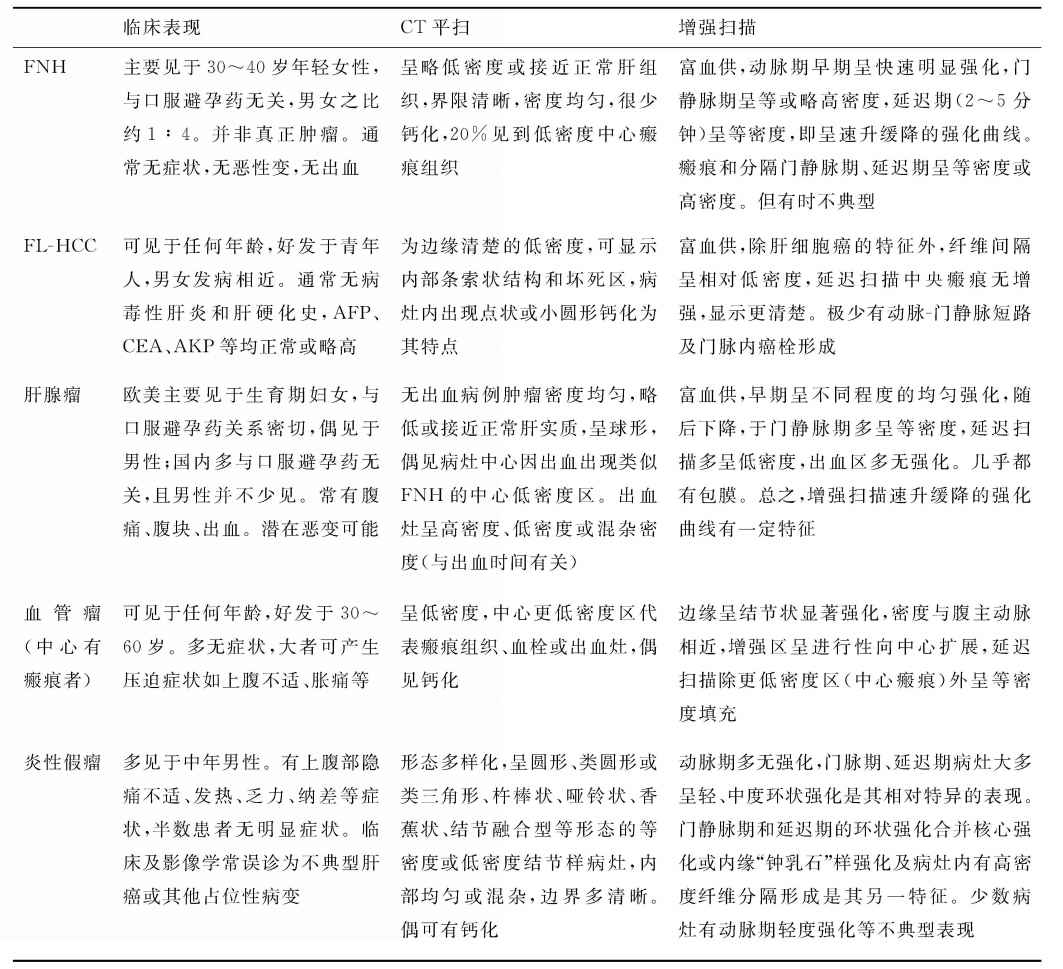
\includegraphics[width=\textwidth,height=\textheight,keepaspectratio]{./images/Image00280.jpg}
\end{table}

\subsection{肝脏囊腺瘤}

肝脏囊性腺瘤样肿瘤有良、恶性之分,分别为囊腺瘤和囊腺癌,都起源于肝内胆管,故又称为胆管囊腺瘤或胆管细胞囊腺瘤(或癌)。

\textbf{【病理】}
囊腺瘤以囊性为主,界限清楚,内含液体,有纤维基质分隔,故为多房性。囊壁薄,纤维组织部分呈乳头状生长,乳头分支少;被覆良性立方或扁平上皮细胞,组织无明显异型性。普遍认为囊腺瘤是囊腺癌的癌前病变。

\textbf{【临床表现】}
有报道多见于30岁以上女性。肿瘤生长缓慢,大者因压迫肝组织或邻近脏器产生上腹部不适、胀痛,或触及肿块。

\textbf{【CT表现】}
CT显示囊实性肿块,边缘清晰,良性者以囊性成分为主,可见壁结节和纤维分隔(图\ref{fig11-9})。增强扫描与囊腺癌一样,肿瘤实质、壁结节及纤维间隔有强化,动脉期强化较著或等于肝,门脉期、延迟期可有持续强化或无持续强化(低于肝脏)。

\begin{figure}[!htbp]
 \centering
 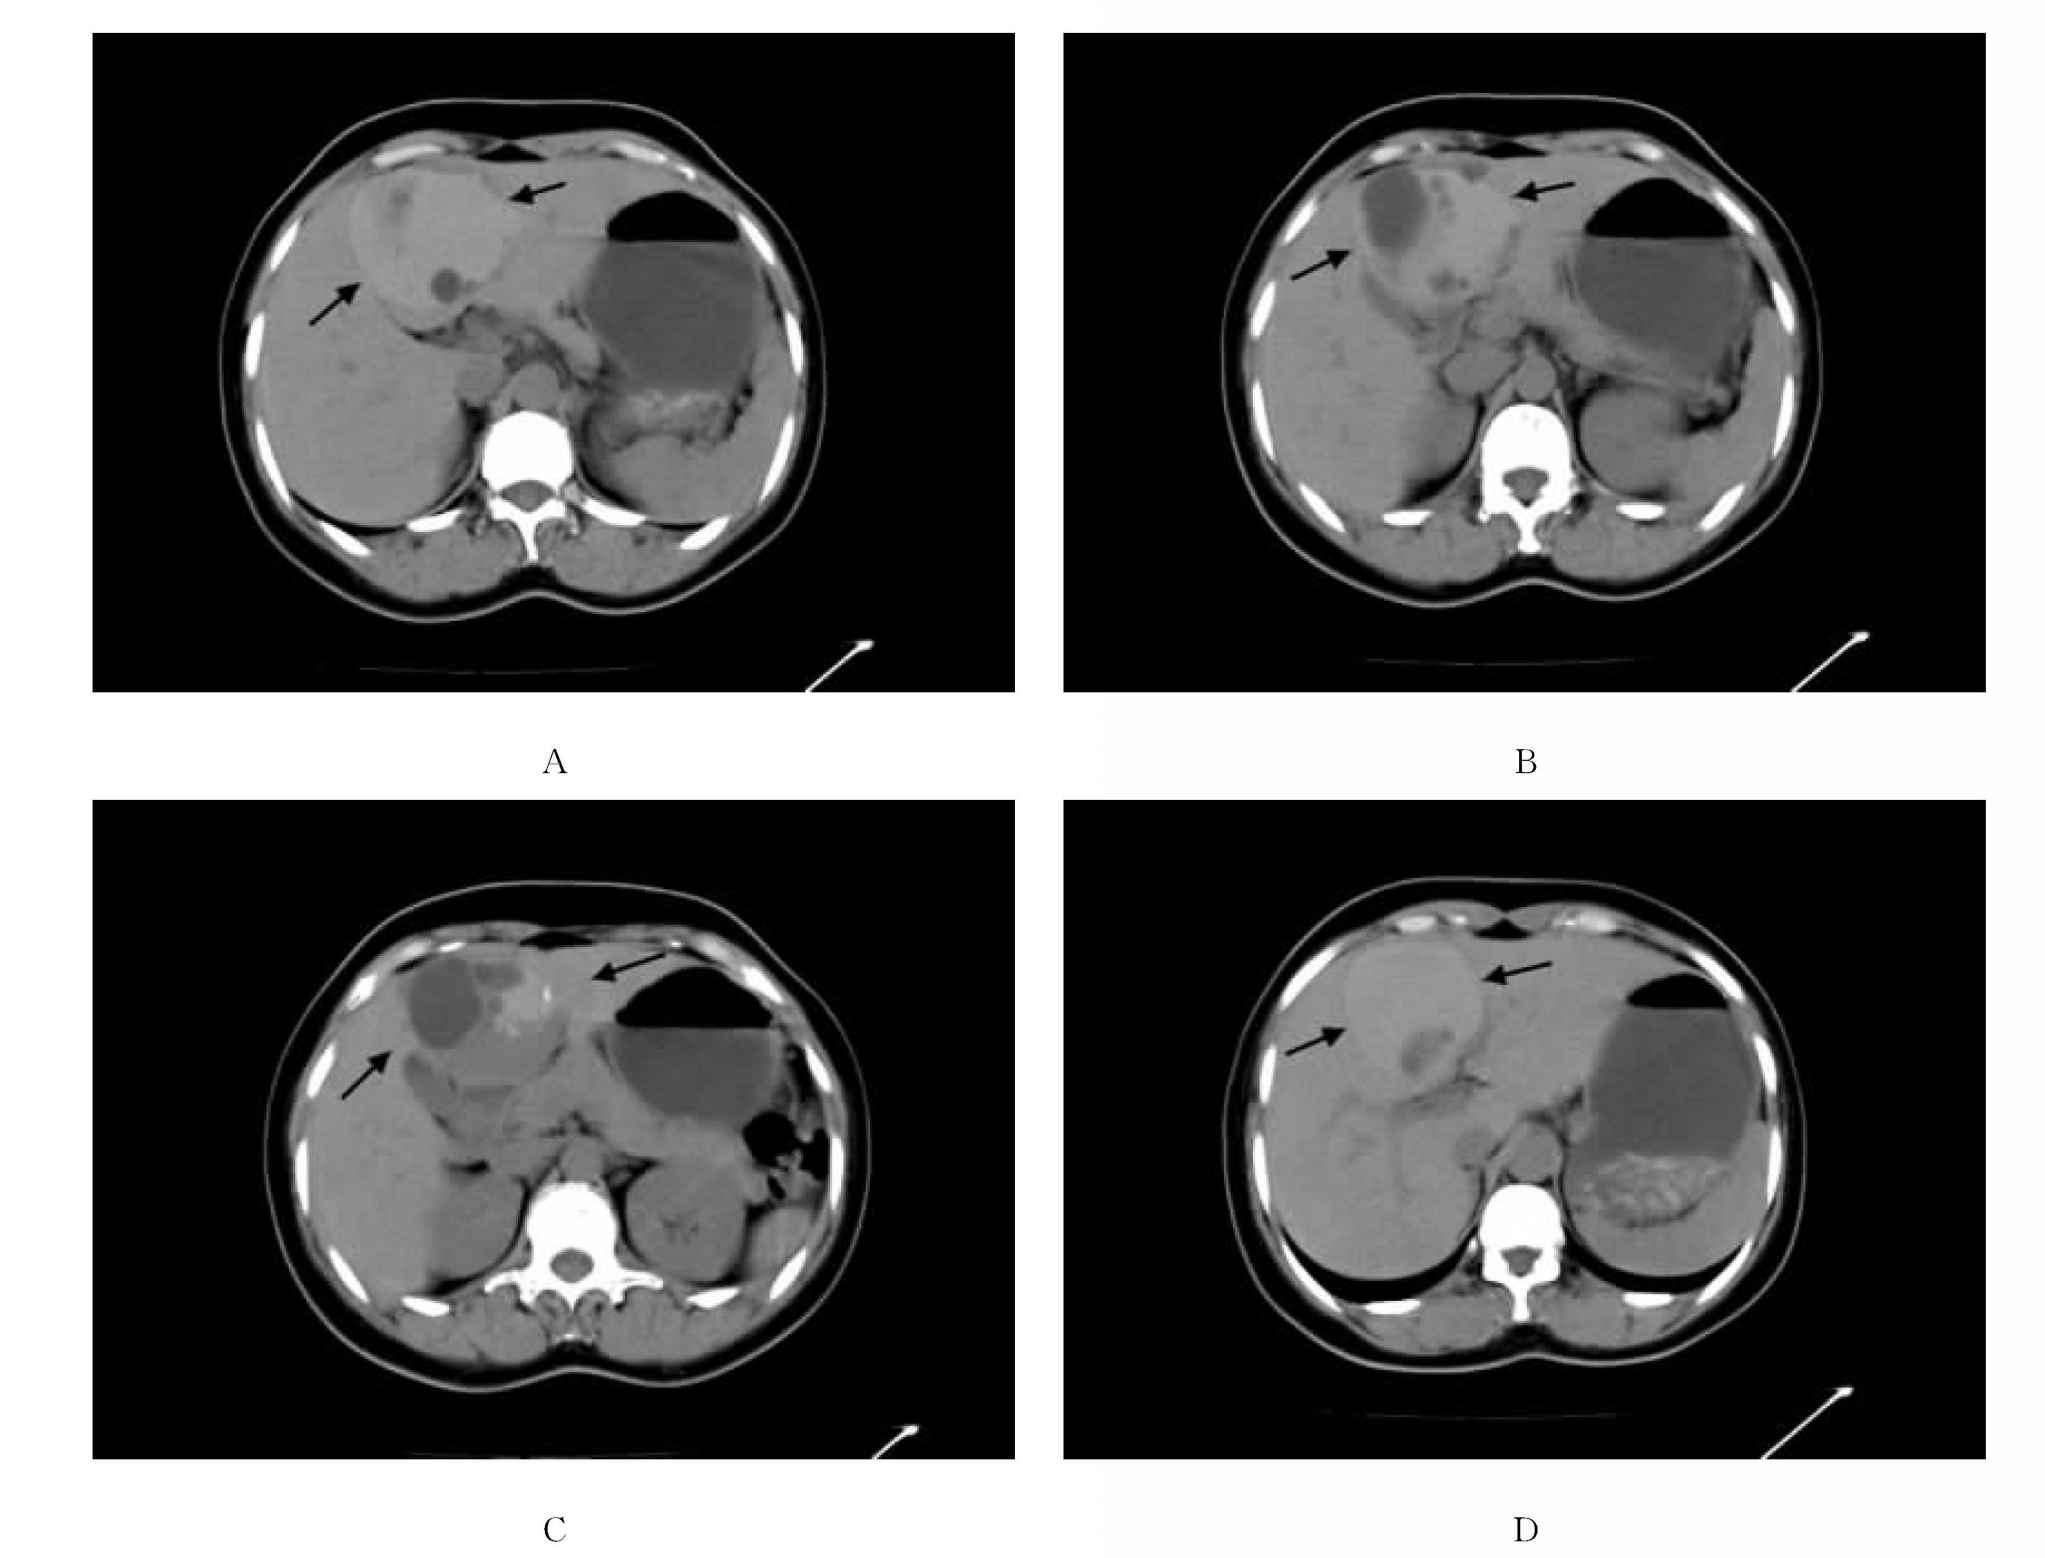
\includegraphics[width=.7\textwidth,height=\textheight,keepaspectratio]{./images/Image00281.jpg}
 \captionsetup{justification=centering}
 \caption{肝脏囊腺瘤\\{\small A~D为同一患者,女,45岁。肝左叶内段有近圆形囊实性密度灶,边缘光整、界限较清晰,近病灶边缘处有斑点状钙化}}
 \label{fig11-9}
  \end{figure} 

\textbf{【鉴别诊断】}
单从影像学囊腺瘤与囊腺癌不易区别,主要依靠病理。如肿瘤内软组织成分多,壁和间隔较厚而不规则,囊内出血以及伴粗大钙化者则恶性可能性大。恶性者还可见周围卫星灶。本病还需和其他囊性肿块如单纯囊肿、包虫病、脓肿、错构瘤及其他囊样肿瘤相鉴别。

\subsection{肝脂肪瘤}

肝脂肪性肿瘤为较罕见的良性肿瘤,代表性疾病为脂肪瘤及血管平滑肌脂肪瘤,其他还有血管髓样脂肪瘤、腺脂肪瘤等。

\textbf{【病理和临床】} 肝脂肪瘤少见,由成熟的脂肪细胞构成。一般无症状。

\textbf{【CT表现】}
平扫可见肿瘤呈边缘清楚的类圆形均匀低密度占位性病变,CT值<-50Hu。增强扫描肿瘤基本无强化。

\textbf{【鉴别诊断】}
脂肪瘤及其他肝脏脂肪性肿瘤,病灶内脂肪成分少者与其他实性肿瘤鉴别困难。此外,还需注意与少见的含脂肪成分的肝细胞癌、肝腺瘤以及局灶性脂肪肝等相鉴别。

\subsection{肝血管平滑肌脂肪瘤}

本病又称为肝错构瘤,罕见。

\textbf{【病理】}
由脂肪、血管及平滑肌3种成分构成。多为单发,亦可多发或伴肾血管平滑肌脂肪瘤。其与结节性硬化的关系尚不清楚,有学者报道10%与肾错构瘤同时并可伴结节性硬化。

\textbf{【临床表现】}
多见于青年女性。有文献报道男女之比约1∶5。临床上常无症状而偶然发现。亦可有上腹部不适、疼痛或包块。

\textbf{【CT表现】}
平扫可见边缘光滑锐利、界限清晰的肿块,密度高低不等,可见血管、软组织、脂肪成分。增强扫描动脉期、门静脉期可见软组织成分轻、中度强化及粗大血管的明显强化,脂肪成分一般无或仅轻度强化。

\textbf{【鉴别诊断】}
①脂肪瘤:边缘清晰、均匀的脂肪密度肿块,无血管及其他成分。②局部脂肪浸润:呈边界不清的低密度灶,无占位效应。③髓脂肪瘤:为乏血管肿块。

\subsection{肝脏良性间叶错构瘤}

本病又称为囊性间充质错构瘤,是除血管内皮细胞瘤外,第二位常见的儿童肝脏良性占位性病变(肿瘤样病变)。可恶变为恶性间叶瘤。

\textbf{【病理】}
肿瘤边界清楚、无包膜,含有多个大小不等的囊性区域,囊腔内含有黏液或凝胶物质,被间充质、异常胆管和肝细胞所组成的纤维基质间隔所分开。

\textbf{【临床表现】}
最常见于3岁以下男孩,可扪及肿块或表现为无痛性的腹部膨隆,常无症状。

\textbf{【CT表现】}
平扫病变呈边缘清楚的低密度囊性肿块,可见分隔,囊壁和间隔光滑、无钙化,囊内密度不一致。也可呈实性肿块,其内有多个大小不等的囊。增强扫描实性部分、较厚的间隔可以强化。

\subsection{肝囊肿}

通常说的肝囊肿为先天性,又称为真性囊肿,不包括创伤性、炎症性、寄生虫性和肿瘤性。肝脏真性(上皮源性)囊肿分为两类:①单纯性肝囊肿:可单发、多发。②多囊肝:又称为多囊病性囊肿,与单纯性多发性肝囊肿含义不同,但两者从影像学角度鉴别困难。多囊肝常合并肾、胰等其他脏器囊肿,尤其多见于肾,为常染色体显性遗传性疾病。

\textbf{【病因病理】}
两类囊肿均可能是胆管在胚胎期发育异常形成小胆管丛,出生后逐渐扩大、融合而成。囊壁一般衬以分泌液体的立方上皮细胞,少数衬以柱状上皮细胞,亦可无内衬上皮细胞,只是纤维囊壁。外被以纤维组织包膜。囊肿大小悬殊大,可小如针尖、大如人头。大囊肿可能由相邻囊肿相互融合而成。多囊肝之囊壁薄,切面呈蜂窝状,约50%合并多囊肾。

\textbf{【临床表现】}
一般无症状。大囊肿或多囊肝者,可有腹部膨隆、肿物及对邻近脏器的压迫症状。合并囊内出血、破裂时可有剧烈腹痛,继发感染时类似肝脓肿症状。多囊肝很少损害肝功能。

\textbf{【CT表现】}

1.单纯性肝囊肿:①呈边缘光滑、境界清晰之圆形低密度灶,囊壁极薄如线状,常不易显示。囊内密度均匀,CT值近于0。增强扫描无强化(图\ref{fig11-10}A)。②小的囊肿因部分容积效应,CT值稍高(可薄层CT确诊);合并感染时囊内容物密度也稍高,囊壁增厚并有强化;合并出血时,囊内密度不均,有高密度区。③大的囊肿压迫肝内胆管可有局限性胆管扩张。

2.多囊肝:可见多发、大小不等的圆形囊肿,病变形态与性质与上述相同,如与多囊肾等同时存在有助于诊断(图\ref{fig11-10}B)。个别可合并出血、破裂,甚至恶变。

\begin{figure}[!htbp]
 \centering
 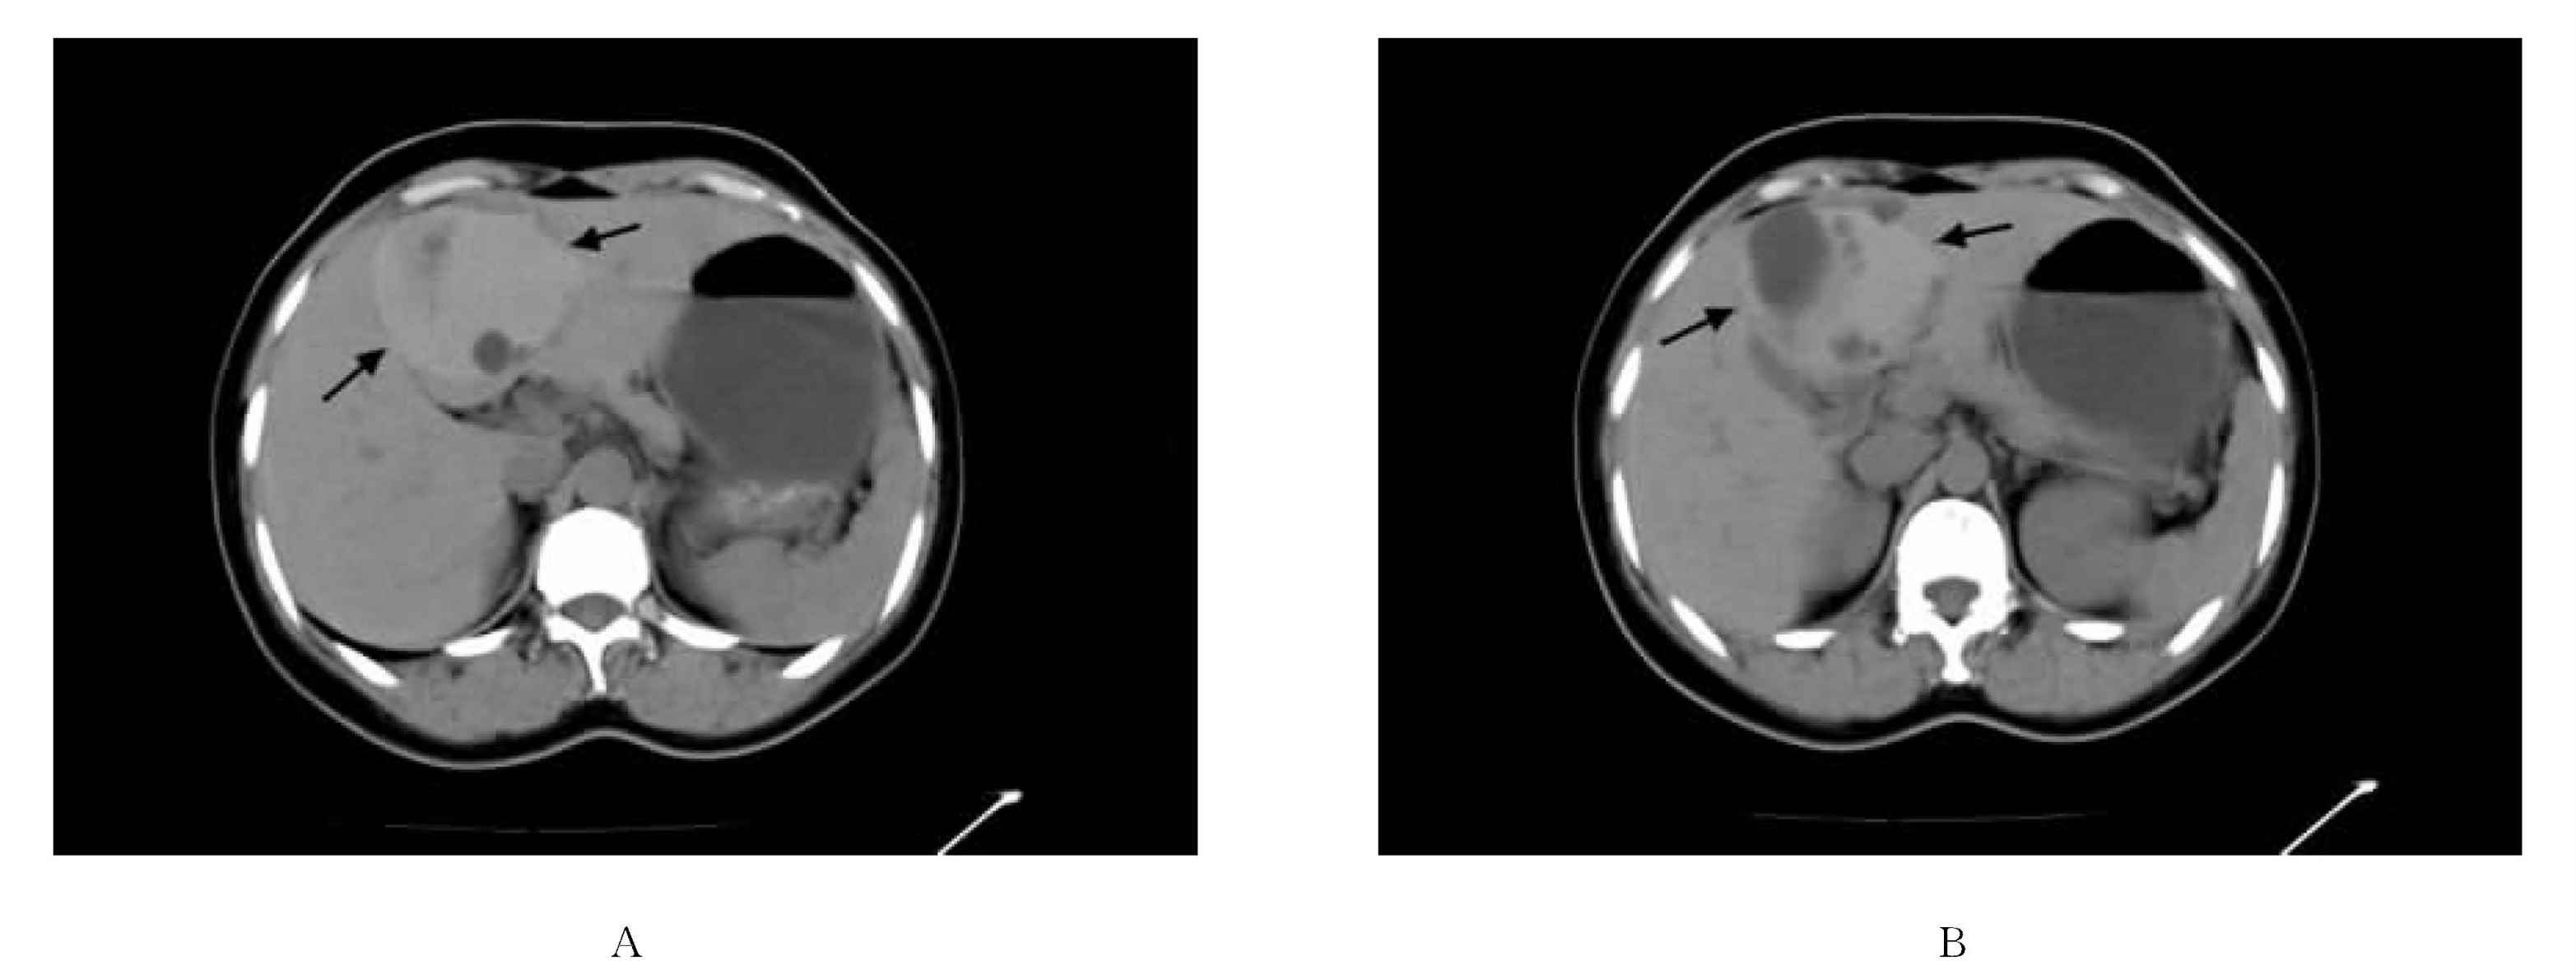
\includegraphics[width=.7\textwidth,height=\textheight,keepaspectratio]{./images/Image00282.jpg}
 \captionsetup{justification=centering}
 \caption{肝囊肿\\{\small A.多发性肝囊肿;B.多囊肝(合并多囊肾)}}
 \label{fig11-10}
  \end{figure} 

\textbf{【鉴别诊断】}
①在平扫或增强图上,边缘清晰的数毫米大小的低密度结节影几乎都是小囊肿,因为如此小的实性占位在平扫图上一般不能显示,至少不清楚。但与扩张的肝内胆管断面可难以区别。②典型囊肿或不典型囊肿(囊肿内出血、感染和分隔),应注意与不典型的肝内囊样病变如囊样转移瘤、肿瘤坏死、囊腺瘤或癌、脓肿、包虫病等相鉴别。注意有无壁肥厚、壁结节、内部间壁、子囊等特征性改变以利于鉴别。③真性上皮囊肿与纤维前肠性肝囊肿、外伤后囊肿、肝内胆汁瘘(胆汁性假囊肿)或其他假性囊肿CT无法鉴别,也无临床意义。

\section{肝脏炎性疾病和寄生虫病}

\subsection{肝脓肿}

肝脓肿主要分为细菌性和阿米巴性两类,前者远为多见。

\textbf{【病因病理】}

1.细菌性肝脓肿:致病菌以革兰氏阴性菌多见。在热带和亚热带如广州和海南还可见类鼻疽假单胞菌肝脓肿(常还累及其他脏器如肺、脾、肾等,且常有糖尿病、白血病、SLE等基础疾病)。

主要感染途径为:①胆道炎症;②经门静脉:所有腹腔内、胃肠道感染均可经门静脉系统进入肝脏,常见的为急性化脓性阑尾炎;③直接蔓延:邻近器官如胆囊等化脓性炎症的直接蔓延;④经肝动脉:全身各部化脓性炎症均可,患者常有败血症。

肝脓肿可单发或多发,单房或多房,右叶远多于左叶。早期病理改变为局部炎症、充血、水肿和坏死,然后液化形成脓腔。脓肿壁由炎症充血带或(和)纤维肉芽组织形成,周围常伴水肿。多房性脓肿由纤维肉芽组织或尚未坏死的肝组织形成房内分隔。

2.阿米巴肝脓肿:继发于肠阿米巴病,溶组织阿米巴原虫经门静脉系统进入肝脏。脓液有臭味、巧克力样。易穿破到周围脏器或间隙如膈下、胸腔、心包腔和胃肠道等。病理所见与细菌性肝脓肿一致。

\textbf{【临床表现】}

1.细菌性肝脓肿:典型表现为寒颤、高热、肝区疼痛和叩击痛、肝大、血白细胞和中性粒细胞计数升高,以及全身中毒症状。少许病例症状不明显。

2.阿米巴肝脓肿:发病前有痢疾或腹泻史,然后出现发热及肝区疼痛,血白细胞及中性粒细胞计数不高,粪便中可找到阿米巴滋养体。

\textbf{【CT表现】}
习惯上人们根据肝脓肿的病程及CT表现,将其分为典型和不典型肝脓肿。

1.典型肝脓肿

脓肿呈圆形、椭圆形或不规则(巨大者可)低密度占位。其中心区域CT值略高于水而明显低于邻近正常肝组织,密度均匀或不均匀。病灶边缘多不清楚。周围可有低密度水肿,少数病灶内有积气等。增强扫描呈单环、双环甚至三环状强化是其特征性表现(图\ref{fig11-11})。在动脉期病灶中心呈低密度区,伴极轻或轻度环状强化。门静脉期强化环更明显,双环者其外侧低密度环开始强化,但强化程度低于内侧强化环和肝实质。实质期强化环仍明显高于周围肝实质,且病灶周围的低密度环可消失,而使病变显示“缩小”。多房脓肿有单个或多个间隔。

\begin{figure}[!htbp]
 \centering
 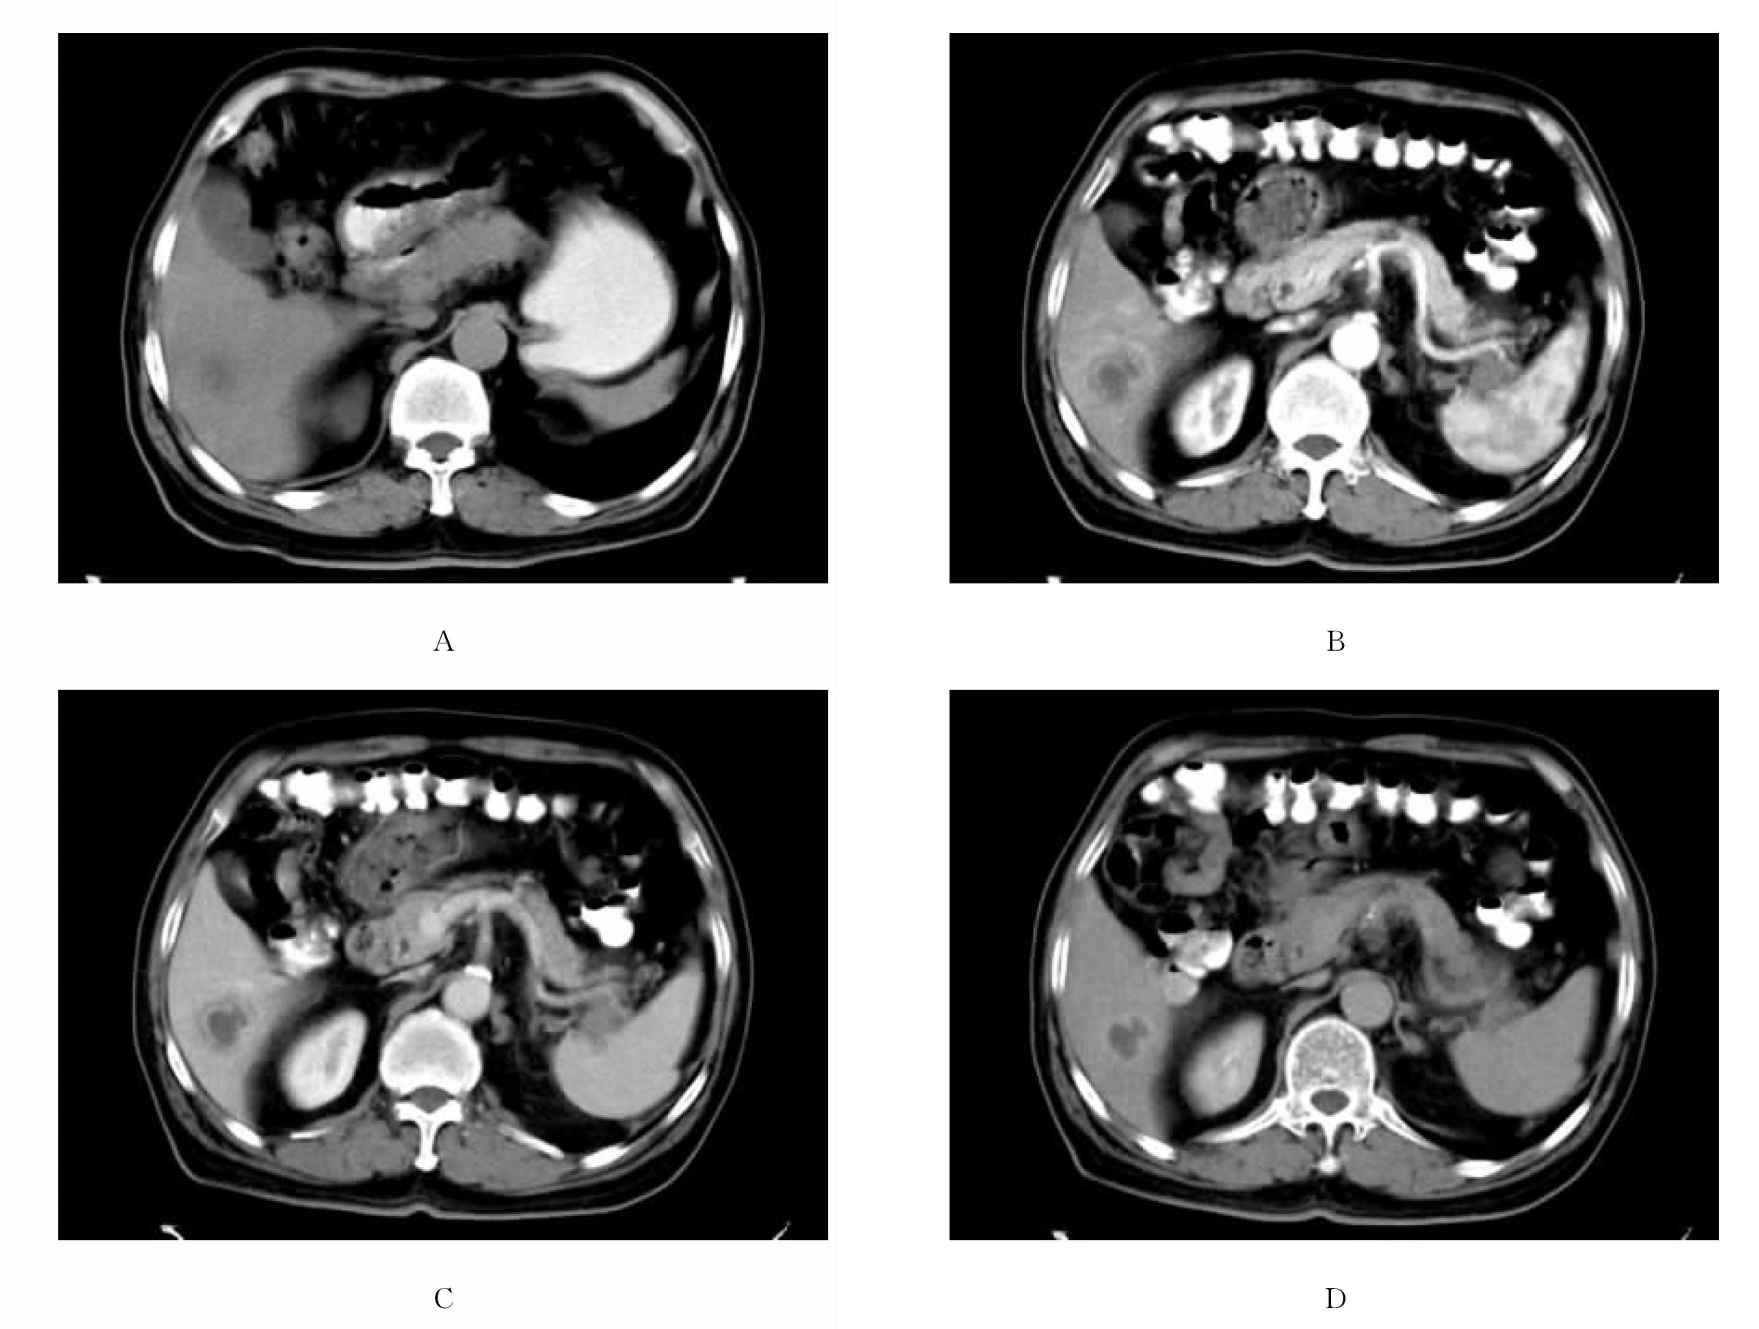
\includegraphics[width=.7\textwidth,height=\textheight,keepaspectratio]{./images/Image00283.jpg}
 \captionsetup{justification=centering}
 \caption{肝脓肿\\{\small A~D为同一患者。A.平扫病灶呈边缘模糊的低密度灶;B.动脉期可见双环征;C.门静脉期仍可见双环征;D.为平衡期(延迟4分钟扫描)强化环仍明显高于周围肝实质,病灶周围的低密度环消失}}
 \label{fig11-11}
  \end{figure} 

一般而言:①单环代表脓肿壁的显示,说明周围水肿带不明显;②双环表明脓肿壁(内环)周围有水肿带(外环)存在,外环的密度低于内环;③三环的出现表明除了水肿带(外环)外,脓肿壁有两层构成。脓肿壁外层(中环)一般为纤维肉芽组织,强化最著;内层(内环)由炎症组织构成,强化不及肉芽组织,如内层有坏死组织构成,则不出现强化。

2.不典型肝脓肿

国内外学者习惯上将具有液化坏死、边缘有双环征、病灶内有积气等称为典型脓肿,否则归为不典型脓肿。不典型脓肿可能与脓肿早期液化不完全、纤维肉芽包膜未形成(故无强化环)、致病菌毒力较低(灶周水肿带不明显)等原因有关。由于抗生素的广泛应用不典型者逐渐增多。

平扫表现无特征性。呈边缘模糊或清晰、密度均匀或不均匀的低密度肿块,CT值多在10~30Hu之间。增强扫描病灶内均见多房近水样更低密度区,以及中心分隔样、斑片状强化。实质期亦可见病灶“缩小”。具体有以下特征:①水样密度房腔有3个特点:其一是绝大多数呈类圆形;其二是边缘多清晰锐利;其三是房腔多紧贴病灶边缘分布,且外缘多达病灶表面而使整个脓肿灶大部分边缘显得清晰锐利。故国内有学者将其称为“周边多囊征”及“边缘锐利征”。②房隔样强化:多呈自病灶中央向边缘伸延的、蜘蛛足状分布的、较细的条索状影,其内端多在病灶中心区互相连接,典型者连接部构成病灶中心蜘蛛体样结构,称之为“蜘蛛征”。③大多延迟至15分钟扫描房隔样结构持续强化,故称之为“持续强化征”。

上述特征均在增强早期及延迟扫描时出现,以病灶中心层面最易显示,但亦有不少作者以蜂窝状表现、簇状征、花瓣征、分隔样强化作为对不典型脓肿的描述(图\ref{fig11-12})。

\begin{figure}[!htbp]
 \centering
 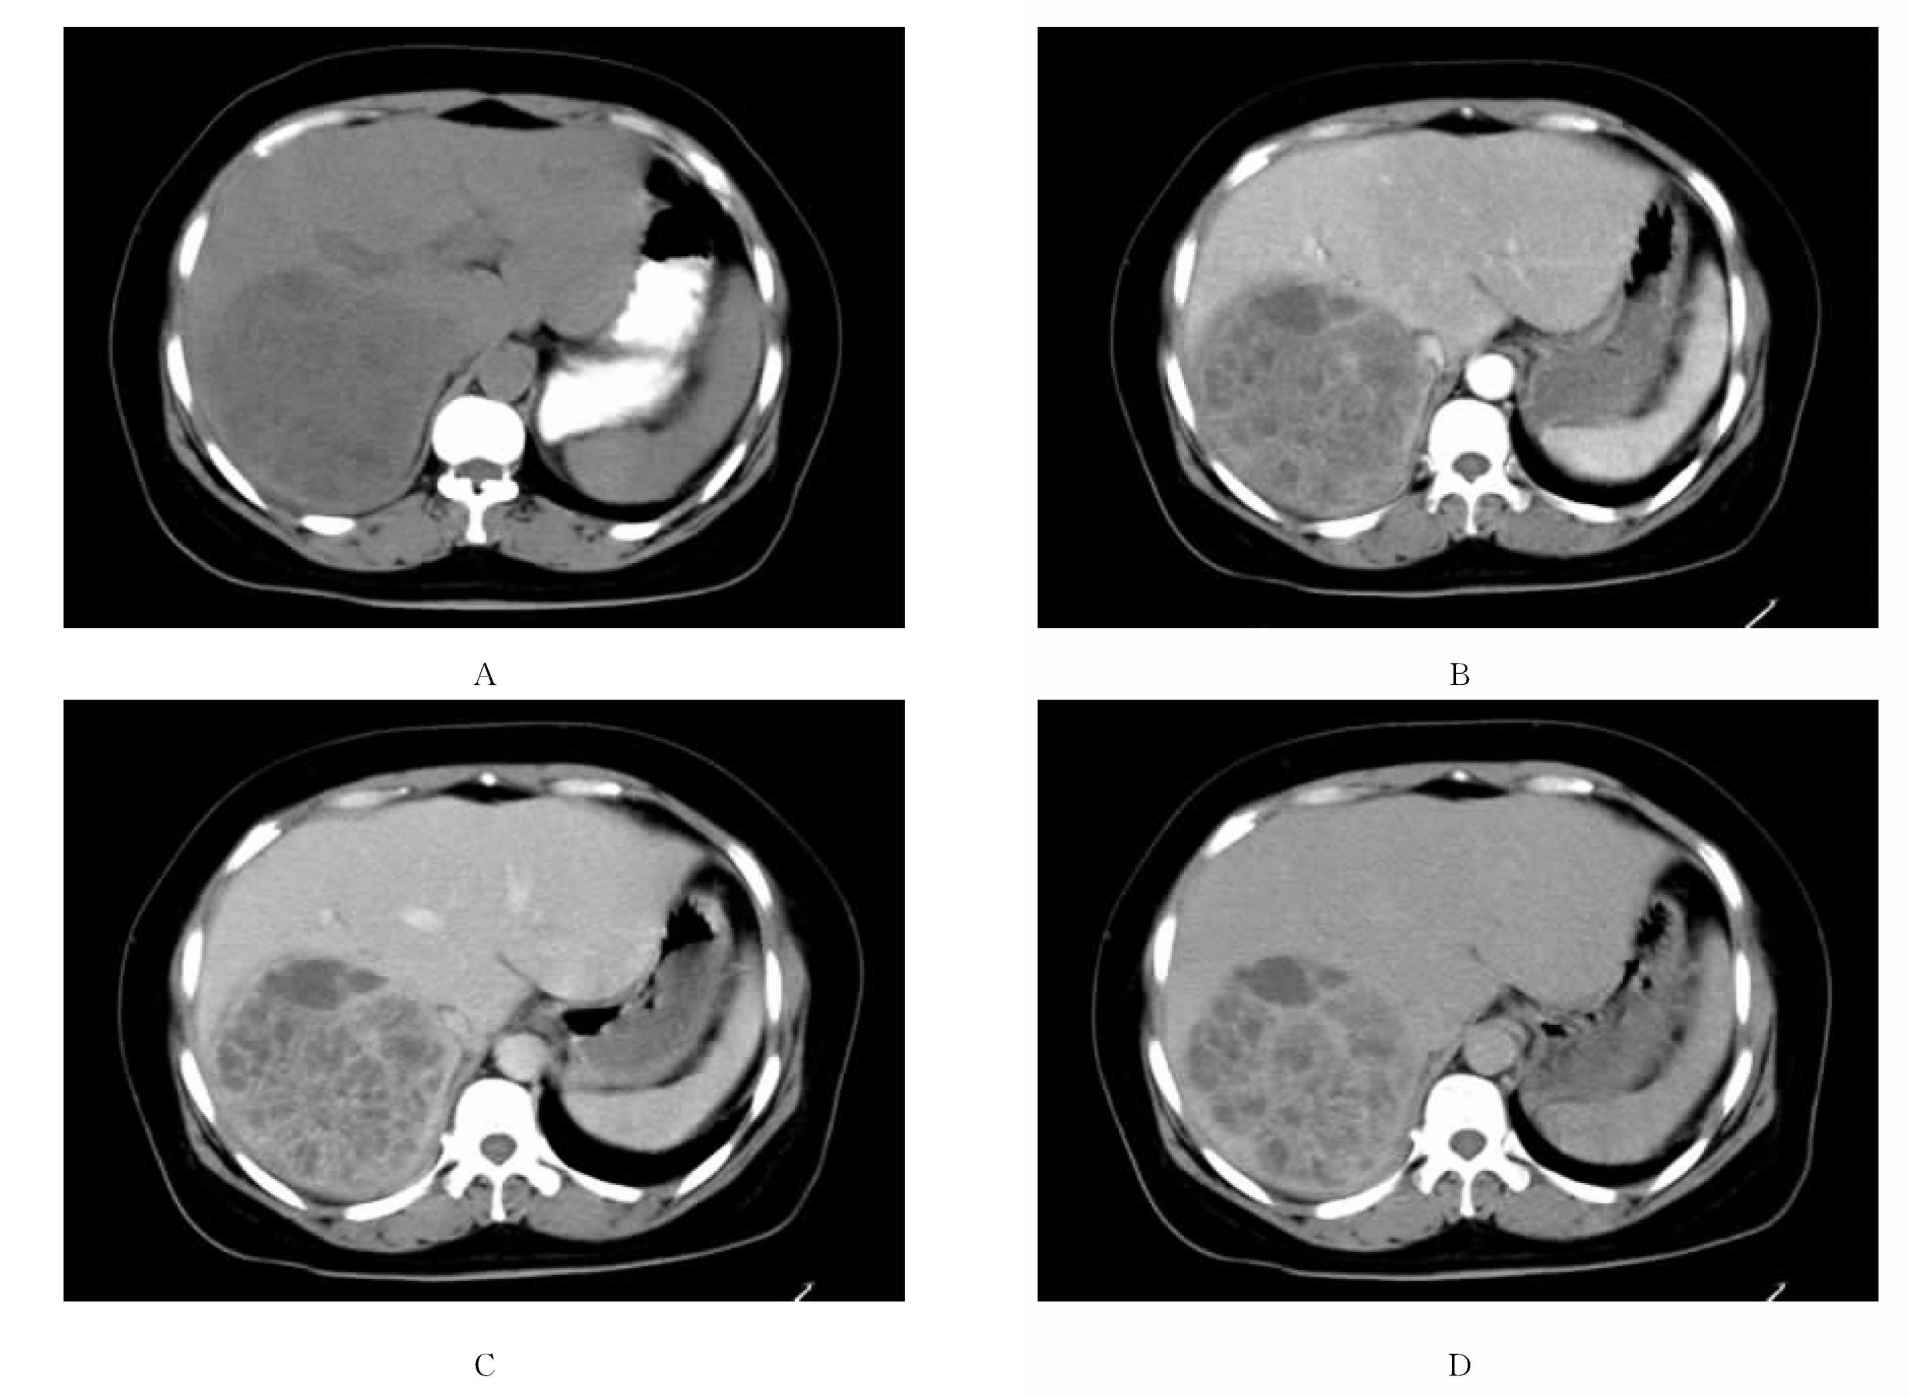
\includegraphics[width=.7\textwidth,height=\textheight,keepaspectratio]{./images/Image00284.jpg}
 \captionsetup{justification=centering}
 \caption{不典型肝脓肿\\{\small A~D为同一患者。A为平扫病灶呈边缘模糊的低密度灶;B、C、D分别为动脉期、门静脉期和平衡期(延迟5分钟扫描),可见病灶呈蜂窝状强化,周围有轻度的低密度水肿环}}
 \label{fig11-12}
  \end{figure} 

3.脓肿周围肝组织一过性段性强化

国内有学者报道近75%的肝脓肿可出现段性强化。表现在增强扫描动脉期,病灶周围的肝实质出现楔形强化,少数为圆形;当多个强化灶邻近时则呈大片状不规则强化区;门静脉期这些强化区消失。这种强化在典型和不典型肝脓肿均可出现。

其病理机制可能是因围绕脓肿周围的门静脉分支有明显的炎性浸润,导致管腔狭窄,从而引起门静脉血流减少和动脉血流代偿性增加所致。

但这种病灶周围的一过性强化,还可见于门静脉分支受压或阻塞、肝静脉阻塞、胆管炎、胆囊炎、肝硬化、血管变异、肿瘤(如HCC、血管瘤)等。应注意结合上述脓肿的典型及不典型表现予以鉴别。

\textbf{【鉴别诊断】}
脓肿早期易与肿瘤混淆,脓肿增强扫描的单环、双环、三环状强化和积气等典型表现,以及周边多囊征、边缘锐利征、蜘蛛征和持续强化征等不典型表现,是与其他疾病鉴别的关键。

1.肝癌:①肝癌坏死区域的CT值一般高于脓液、边缘明显高低不平(但脓肿内壁亦可不规则)、强化曲线多呈速升速降型、强化持续时间短等有别于脓肿的上述典型及不典型表现。②脓肿强化持续时间长,明显有别于肝癌。③增强扫描肝癌病灶多无缩小趋势,而脓肿常见。④掌握上述不典型脓肿之特殊表现,亦是与胆管细胞癌鉴别的关键。

2.肝转移瘤:囊性转移的病灶边缘多强化,如为单个或病灶数目不多,尤其是具有“牛眼征”者可与脓肿混淆。但转移灶周围无水肿带,结合病史及临床症状多可鉴别。

3.肝囊肿:少数脓肿边缘清晰,需与囊肿鉴别。但脓肿的某一边缘总是模糊的,边缘有强化,密度稍高于单纯囊肿。如囊肿继发感染则两者极为相似,治疗后边缘转为清晰,且大小无变化,则支持囊肿诊断。

\subsection{真菌性肝脓肿}

真菌致病力很弱,只有机体抵抗力下降时,真菌进入血液循环到达肝脏引起感染,才能形成真菌性肝脓肿。

\textbf{【病理】}
本病主要是真菌在肝组织内产生变态反应,引起肝组织损伤、坏死,形成多发、大小不等的脓肿,脓肿壁一般较厚,有组织细胞、淋巴细胞浸润。有时脓肿可形成真菌性肉芽肿。

\textbf{【临床表现】}
多无特异性症状。一般起病缓慢,可有肝大、发热以及肝功能损害。

\textbf{【CT表现】}
平扫显示肝实质内多发、散在的小低密度灶。增强扫描脓肿壁无强化或少数边缘轻度强化。有时脓肿中心可见点状高密度影,可能是霉菌丝积聚影,称为“靶征”。肉芽肿愈合可出现高密度钙化。

\subsection{肝结核}

肝结核为结核病全身性播散之局部表现,患者常同时患肺结核或肠结核。据统计约50%~100%粟粒性肺结核患者同时合并肝结核。其感染可经血行、淋巴及直接侵犯等途径进入肝脏。

\textbf{【病理】}
一般先产生弥漫性粟粒性肝结核,因胆汁有抑制结核菌生长的能力,且肝脏抗结核能力也强。故一般病情趋向好转、钙化及治愈;若病情恶化,则小结节扩大、相互融合,中心发生干酪坏死,形成结核性脓肿。以后,脓肿被纤维组织包绕,形成结核瘤;亦可穿入胆道,产生结核性胆道炎症;还可穿入胸、腹腔。

\textbf{【临床表现】}
多无特异性症状。一般起病缓慢,重者有低热、乏力、盗汗、消瘦、肝区疼痛,血沉快。

\textbf{【CT表现】} 其CT表现多为非特异性的,有以下3类。

1.粟粒型:此型最常见。肝肿大伴多发性粟粒状低密度灶;或肝大伴密度减低,而多发的小病灶显示不清。此型如无肝外结核存在,多不能确诊。绝大多数经药物治疗后吸收、纤维化、钙化。有学者注意到血行播散型结核累及肝脏主要表现为均匀增大,较少有散在低密度灶;而脾、肾受累常形成低密度灶。

2.结节型:①平扫呈结节状低密度灶,或密度不均之混合密度灶,病变单发或多发。增强扫描轻至中度边缘强化。②结核性肝脓肿:病灶中心坏死可形成结核性肝脓肿。增强扫描动脉期病灶边缘及分隔强化明显,而门静脉早期强化降低,远不如肝实质的强化;门静脉后期、平衡期病灶边缘及分隔轻度强化,分隔影增厚、病灶缩小。结核性肝脓肿亦可呈“双环”表现,而难以与其他肝脓肿鉴别。

3.混合密度型:①呈类圆形2~5cm大小的结节状病变,中心为高或等密度,并可有斑点状或粉末状钙化,有报道粉末状钙化是肝结核的特征性表现。②周围低密度,边缘有一均匀的薄环,并可有环状强化表现。③结核性胆管炎极为少见,可呈沿胆管壁走行的钙化。

此外,腹腔淋巴结增大(呈环状或多个环状强化)、病变周围卫星灶及肝外其他结核有助于诊断和鉴别诊断。

\subsection{肝脏炎性假瘤}

本病又称为肝脏炎性肌纤维母细胞瘤、浆细胞性肉芽肿、纤维组织细胞瘤、纤维黄色瘤等。本病较为少见,于1953年首先由Pack等报道。

\textbf{【病因病理】}
曾有人认为与感染有关,与复发性化脓性胆管炎及闭塞性静脉炎关系密切,可能是对肝内细菌感染的异常组织反应;目前多人认为可能是一种自身免疫性疾病。病理上是由各种致炎因子引起的局部肝组织的炎性细胞浸润、凝固坏死、肉芽肿形成和纤维组织增生为特征的肿瘤样病变。炎性细胞包括浆细胞、淋巴细胞、嗜酸性细胞及吞噬细胞。病灶多为单发,少数为多发(20%)。以肝右叶常见。

\textbf{【临床表现】}
可发生于任何年龄,多见于婴幼儿和青壮年男性,国外报道男女比例约29∶1,但国内报道1组为3∶2。有上腹部隐痛不适、发热、乏力、呕吐、纳差、全身不适、体重下降等症状,以发热多见,且多为高热。如累及胆管可有黄疸。近半数患者无明显症状而偶然发现。实验室检查多数WBC升高,ESR增快,C反应蛋白阳性等;肝功多正常。临床及影像学常误诊为不典型肝癌或其他占位性病变。

\textbf{【CT表现】}
病灶常局限于一个肝叶,以右叶多见,左叶和肝门区亦可发生。病灶大小多在2~14cm。有人认为有症状者(平均8.3cm)大于无症状者(平均3.6cm)。

1.平扫:呈等或低密度结节样病灶,内部均匀或混杂,偶可有钙化,边界多清晰。形态多样化,呈圆形、类圆形或类三角形、杵棒状、哑铃状、香蕉状、结节融合型等。

2.增强扫描:其表现复杂多样。动脉期多无强化,门脉期和延迟期病灶大部分呈中心部弱强化、边缘部相对明显的轻、中度环状强化是其相对特异的影像学表现。国内还有学者认为门静脉期和延迟期病灶的环状强化合并核心强化或内缘“钟乳石”样强化,以及病灶内有高密度纤维分隔形成是其另一特征。病灶也可均匀强化、不均匀强化(其内可有高密度分隔)或无明显强化。少数病灶动脉期轻度强化,可能与其中凝固坏死少而炎性细胞浸润相对较多,或病灶内含有一定肉芽组织有关。国内还有学者报道1例,动脉期呈显著强化,随后迅速下降呈等密度,而边缘包膜及中央瘢痕延迟强化,与肝局灶性结节增生(FNH)的动态增强相似。也有报道病灶始终无强化。

因病灶中央主要为纤维组织和炎性肉芽肿,没有肝动脉供血,故早期多无强化表现。因病灶有较多的纤维组织和毛细血管,所以门脉期和延迟期都能见到病灶周围轻、中度的环状强化,这是由于造影剂进入血管外不能迅速廓清所致。

\textbf{【鉴别诊断】}
①肝转移瘤:由于肝转移瘤常伴丰富的纤维组织,亦可出现边缘环状强化,故两者常混淆。但仔细辨别病灶内有无核心强化和纤维分隔等有助于定性和鉴别。②肝脓肿:具有典型临床表现和CT表现者不难鉴别,但不典型者常很难与炎性假瘤鉴别。此外,有时与乏血供的肝癌不易鉴别。③应注意与FNH、纤维板层样肝癌鉴别。

\subsection{肝脏坏死性结节}

本病较少见。

\textbf{【病因病理】}
肝脏结节性坏死主要为炎性肉芽肿及肝内小血肿,以结核性肉芽肿最常见。病变最初为组织内巨噬细胞增生,后变为类上皮细胞并围绕成境界清楚的小结节,小结节内有残存的肝细胞再生及新生的细小胆管等。结核性肉芽肿的中心常发生干酪坏死、钙化。

\textbf{【临床表现】}
国内有学者报道1组,见于青壮年。多无症状,可有上腹部不适。

\textbf{【CT表现】}
①平扫单发或多发不规则、类圆形低密度灶,直径多<4cm。②密度不均匀,内可见点、片状钙化,边缘清晰。③占位征象不著,多数病灶可见一个以上边缘平直或凹陷,相邻血管或胆管无推移,位于肝边缘处无突起征象。④因病灶以纤维增殖为主,基本无肝动脉供血,故增强扫描动脉期无明显强化,延迟期轻度均匀强化,但低于肝实质。⑤半年或更长时间复查,病灶钙化、缩小,甚至消失。

\subsection{肝包虫病}

包虫病即棘球蚴病,是一种人畜共患的寄生虫,可分为两类。①囊型包虫病:由细粒棘球蚴绦虫感染引起的囊型包虫病,又称为棘球蚴、单房型包虫。②泡型包虫病:由泡状(或多房状)棘球蚴绦虫感染所致,又称为包球蚴、多房型包虫,该型很少见。

\textbf{【病理】}

1.囊型包虫病:细粒棘球蚴在肝内以包裹的膨胀方式逐渐长大,包虫囊肿的壁分为内囊和外囊。内囊系棘球蚴本身形成的囊,甚薄,由内外两层组成,内层为生发层,外层为角质层。角质层具有保护和渗透作用,生发层向囊腔内长出雏囊。外囊为包围囊虫的肝组织形成的纤维组织层,生长较久的外囊常发生钙化。

2.泡型包虫病:泡状棘球蚴在肝内呈弥漫性浸润性生长,由无数小囊泡聚集而成,没有大囊或纤维组织层包绕,与正常肝组织界限不清。小囊泡常因病程较长,囊壁有颗粒状及无定形钙化。大的病灶中心可因组织变性或坏死而形成空腔。

\textbf{【临床表现】}
早期,囊型发展缓慢,可长期无症状;泡型症状出现早,主要为过敏反应症状,如荨麻疹、哮喘、恶心、呕吐、休克等。进展期可出现肝脏及邻近脏器压迫性症状。包虫破入不同的脏器、组织而临床表现不同。常破入胸、腹腔,还可破入胆系引起胆管扩张和黄疸。血嗜酸细胞增高、包虫间接血凝试验及补体结合试验多为阳性。晚期常可经过血行或淋巴途径转移到其他器官,如脑、肺和肾、肾上腺和纵隔等。

\textbf{【CT表现】}

1.囊型肝包虫病

(1)基本表现:平扫可见单发或多发圆形、椭圆形或分叶状低密度灶,边缘光滑锐利,界限清晰,大小不一。单房或多房性。囊壁厚度不一,与肝实质呈等密度而不易区分。内容物呈水样,有的很均匀而不易与单纯囊肿相鉴别。干酪或感染时内容物密度升高。增强扫描囊壁及囊内分隔有强化。

其特征性表现为囊内密度不均,囊内有子囊或囊内有分隔而呈多房性。囊内可有软组织团块。

(2)囊内子囊征象:①子囊囊液密度较母囊低,呈母囊内多个小圆形更低密度灶或环状边缘。子囊少时,靠近母囊内壁排列呈车轮状;子囊多时,于母囊内呈葡萄状小囊结构。②若子囊大又多,而填满母囊,由于相互挤压则由球形变为方形或菱形,呈蜂窝状分隔。这都是本病的特征性表现。

(3)钙化表现:可见环状、半环状囊壁钙化,还可见索条状内容物钙化、子囊钙化以及团块状整个包囊钙化。

(4)内囊分离表现:因感染或损伤可造成内囊分离,表现为:①双边征;②水上荷花征;③飘带征;④水蛇征。

(5)并发症:以感染常见,表现为:①囊内密度增高;②囊壁增厚;③偶见气泡影或液气平面。

此外,还有人将其分为无子囊型、内囊分离型、多子囊型、实质钙化型,这4型反映了本病的自然演变过程。

2.泡型肝包虫病

(1)特征性改变:地图样浸润的实性低密度灶,界限不清,包膜不明显。增强扫描无强化。可见到不规则和结节状、点状丛集钙化,而不像囊型多呈环状钙化。病变还可扩展到腹壁、膈、肝门,因此很像肝脏的肿瘤浸润。

(2)大囊肿性病变:平扫呈类圆形低密度病变,周边密度略高,但仍低于肝组织。增强扫描边缘轻度增强为肉芽组织,其内液化坏死区更清晰。有时可见边缘部环状排列的细颗粒状、多结节状或块状钙化灶。

(3)实质性病变:伴有钙化的低密度病变,钙化呈散在分布的结节状、颗粒状。伴有坏死的实质性病变,坏死部分无强化。亦可呈大小不等的圆形低密度集合体,边缘有轻微强化。

此外,该型还可对门管系统及下腔静脉有侵犯征象;转移到其他脏器可有相应的表现。

国内还有学者将该型分为3类:①巨块型:包括实性肿块型、肿块液化型、钙化型;②结节型;③混合型:即巨块合并结节状病灶。并认为泡型肝包虫病的CT特征性表现为病灶内小囊泡和点状、丛集状钙化。

\subsection{肝血吸虫病}

本病即血吸虫寄居在门静脉系统,虫卵随血流沉积于肝内,引起门静脉小分支阻塞。

\textbf{【病理】}
虫卵主要栓塞在汇管区,导致炎症、肉芽组织、纤维组织增生,以及汇管区扩大,破坏肝组织,造成肝组织营养不良,最终导致肝硬化、门静脉高压。

\textbf{【临床表现】}
早期主要为虫卵及虫体引起的组织反应及过敏反应,有发热、肝区痛、末梢嗜酸细胞增多等。晚期主要为肝硬化及门静脉高压症状。

\textbf{【CT表现】}
①肝硬化及门静脉高压表现。②肝内钙化:呈线状、蟹足状、地图状、包膜下及团块状钙化。肝内钙化为晚期血吸虫病肝硬化的基本病理特征和诊断的主要依据。③肝内汇管区低密度灶及中心血管影:虫卵在汇管区沉积,造成纤维化反应,致汇管区增宽和密度下降,其内的门脉分支扩张迂曲。平扫可见肝内0.5~1.0cm的低密度灶,CT值<20Hu,部分为负值,其中心血管呈小圆形影,以增强扫描为著。④门静脉系统钙化:门静脉高压时部分虫卵随血流逆流到脾静脉和肠系膜上静脉,故两者管壁亦可钙化。⑤肠系膜改变:因纤维化反应产生增厚、收缩,甚至大饼样肿块。多伴有大量腹水。⑥结肠壁增厚钙化:呈线状或弧形,主要累及左半结肠。⑦合并肝占位:可合并肝癌,但与肝癌的关系有争议;还可合并血管瘤和囊肿。

\subsection{肝囊虫病}

肝囊虫病少见,有散在报道。

\textbf{【临床表现】}
可有上腹部疼痛。血清酶免疫试验(ELISA)囊虫IgG(+),而包虫等其他寄生虫IgG(-)有助于确诊。

\textbf{【CT表现】}
肝内散在、弥漫的细小囊状低密度灶,直径0.2~1.2cm,多<1.5cm,CT值多为10~20Hu;囊内或囊壁可见针尖大小壁结节(头节)。增强扫描壁结节更清晰,囊内无强化,胆管无扩张。肝脏有时可增大。

\subsection{肝弓形虫病}

弓形虫生活史以猫、狗为终末宿主,而哺乳类、鸟类和人类为其中间宿主。其感染途径有先天性和获得性两种。

\textbf{【病理】}
实验研究表明,弓形虫损害肝脏的重要途径是虫体在组织血管和毛细血管周围的肝细胞内寄生、繁殖,导致肝细胞发生肿胀变性,细胞破裂形成坏死区,以及周围组织的肉芽肿样炎性病变;晚期会导致血管壁破坏、肝内广泛出血等。

\textbf{【临床表现】}
先天性感染多为弓形虫经血流穿过胎盘感染胎心,致不良妊娠等恶性结果,发生流产、早产、死胎和各种胎儿畸形。获得性弓形虫病临床表现多样,以发热、干咳、纳差、体重减轻为主,可侵犯眼、脑、淋巴结等全身器官。肝脏受侵可有肝大、纳差等症状。获得性有长期喂养猫、狗等宠物史。血清酶免疫试验(ELISA)弓形虫抗体IgG、IgM阳性是确诊的关键。

\textbf{【CT表现】}
由于局部肝组织细胞坏死液化,平扫肝内出现多发片状、不规则状低密度灶。增强扫描病灶无明显强化,门静脉期随着正常肝实质的强化,病灶显示更清晰。

应注意与肝炎和早期多发性肝脓肿相鉴别。

\section{肝脏弥漫性病变及血管病变}

肝脏弥漫性疾病根据大体病理可分为4类:①弥漫均匀型:如脂肪肝、血色素沉着症、糖原沉积症等;②节段型:脂肪肝、亚急性肝炎等;③弥漫结节型:病毒感染后的肝硬化、肝豆状核变性、结节病、布加综合征等;④血管周围型:肝淤血、日本血吸虫病等。

\subsection{肝硬化}

本病为慢性弥漫性肝病发展过程中的后期阶段。

\textbf{【病因病理】}
肝硬化是以广泛结缔组织增生为特征的一类慢性肝病。其病因甚多,如肝炎、酒精和药物中毒、胆汁淤积、肝脏淤血及其他少见原因(代谢、寄生虫病等),国内以乙型肝炎为主要原因。

主要病理改变为肝细胞变性、小灶性坏死,肝细胞再生、结构改建及纤维结缔组织增生,形成假小叶。肝表面弥漫分布细小或大小不等的再生结节,小者1~2mm,大者1~2cm。结节之间为纤维结缔组织。肝脏体积缩小、变硬,尤以肝右叶为著;尾叶相对增大。因纤维结缔组织增生及肝细胞再生结节压迫,引起肝内静脉小分支阻塞,使门静脉血流受阻而导致门静脉高压,产生侧支循环及静脉曲张。病理学按病变形态不同分为:①小结节型:相当于门静脉性肝硬化,再生结节大小<1cm;②大结节型:相当于坏死后性肝硬化,再生结节大小约1~3cm,肝明显变形;③混合型:多为坏死后性肝硬化,大小结节共存。

\textbf{【门静脉高压的侧支循环】}
正常情况下,门静脉属支与体循环之间存在着交通支,但门静脉血流都流入肝脏。门静脉高压时,因血流受阻,门静脉血流则经过这些交通支逆流到体循环系统。

主要途径有4条:①经食管静脉、胃左静脉(胃冠状静脉)、胃后静脉与腔静脉系统的肋间静脉、膈静脉、奇静脉、半奇静脉交通,是最主要的侧支循环;②经脐静脉、脐旁静脉(附脐静脉)与胸壁、腹壁静脉交通,以脐为中心向上或向下走行,犹如水母状;③经脾静脉、胰静脉、胃静脉与膈静脉、左肾上腺静脉、肾静脉交通;④腹腔脏器包括肝-膈的Sappy静脉、肠壁(Retzius)静脉丛可将门静脉、肠系膜上下静脉与体循环的腰静脉、膈静脉、肾上腺静脉、肾静脉相交通。

\textbf{【临床表现】}
①慢性肝病症状:早期可无明显症状,晚期有肝功能异常、黄疸、发热、腹水、肝昏迷等;②脾大、脾功能亢进症状;③门静脉高压:侧支循环形成,静脉曲张表现;曲张静脉可破裂导致上消化道出血。

肝硬化的CT表现与临床症状和肝功能紊乱可不一致,即CT表现可先于临床诊断,或者反之。CT表现正常不能否定肝硬化的临床诊断。

\textbf{【CT表现】}

1.肝脏大小和形态:①肝各叶大小的比例失常。由于肝右叶和左叶内段缩小,肝门及叶间裂增宽。尾状叶和左叶外侧段增大,尾叶与右叶横径的比例在0.65以上时,有96%的把握诊断为肝硬化。有学者认为尾状叶的增大是肝硬化的特征性表现。晚期也可普遍萎缩(图\ref{fig11-13})。②结节增生显著者,肝表面明显凹凸不平,边缘变钝,呈分叶状或扇贝形。

\begin{figure}[!htbp]
 \centering
 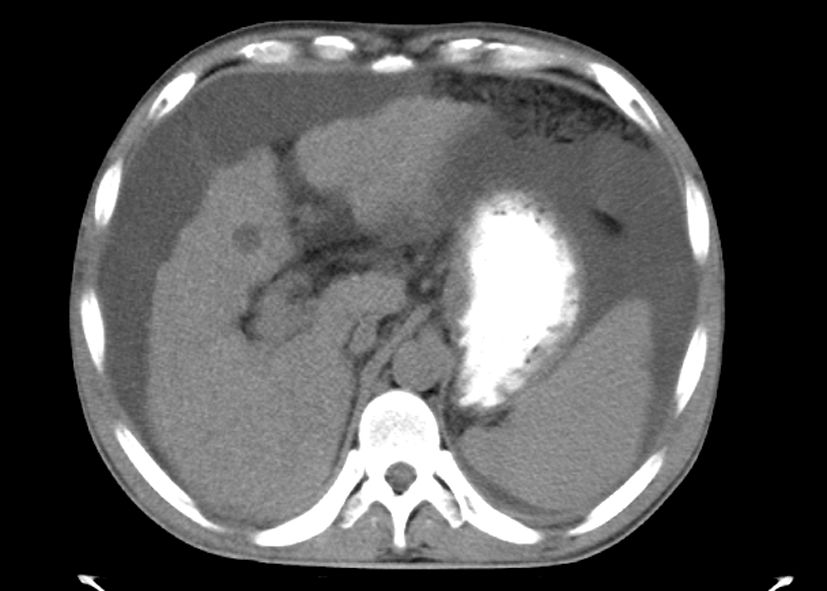
\includegraphics[width=.7\textwidth,height=\textheight,keepaspectratio]{./images/Image00285.jpg}
 \captionsetup{justification=centering}
 \caption{肝硬化并腹水\\{\small 肝脏体积缩小,边缘凹凸不平;肝脾周围有水样密度区}}
 \label{fig11-13}
  \end{figure} 

2.肝脏密度:纤维化、结节再生、变性坏死和脂肪变性等病理改变常致肝密度高低不均。肝硬化再生结节呈相对高密度。结节型肝硬化需注意结合增强扫描与弥漫性肝癌鉴别。

3.继发性改变:①脾大;②腹水;③门静脉高压;④胃肠道管壁增厚:常见于失代偿期,右半结肠好发,白蛋白水平降低及门脉高压可能是其发生的原因。

4.门静脉高压的CT表现:①主要表现为门脉主干及分支扩张,门静脉主干宽径>13mm;脾静脉(宽径>10mm)和肠系膜上、下静脉的曲张、扩张;脾大(图\ref{fig11-14})。②其次为侧支循环血管的建立扩张。

\begin{figure}[!htbp]
 \centering
 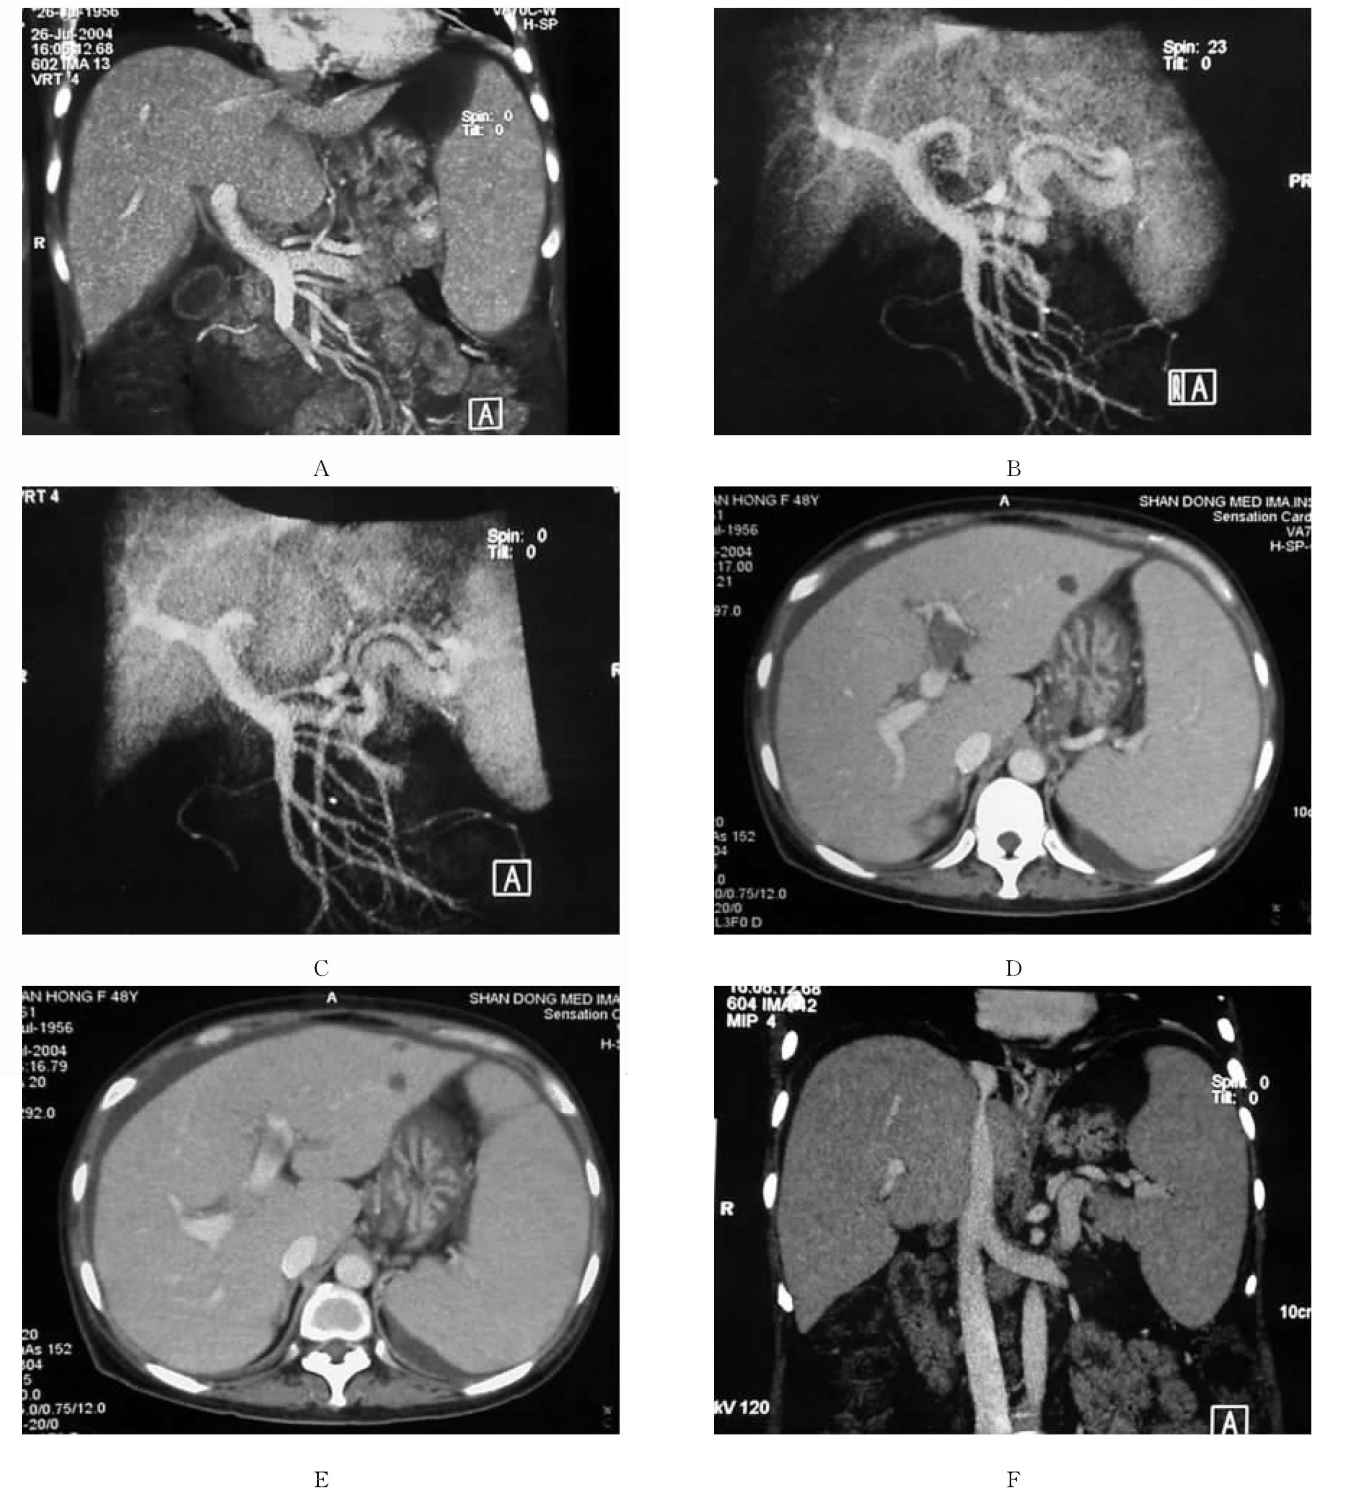
\includegraphics[width=.7\textwidth,height=\textheight,keepaspectratio]{./images/Image00286.jpg}
 \captionsetup{justification=centering}
 \caption{门静脉高压\\{\small 门静脉、脾静脉显著扩张,并可见迂曲扩张的侧支循环血管;门静脉左支栓塞}}
 \label{fig11-14}
  \end{figure} 

扩张的侧支循环血管表现为:①食管下端和食管周围静脉曲张:表现食管外形不规则或分叶状、壁厚;增强可见向腔内、外突出的结节状、条状、蚯蚓状、簇状血管影;可伴奇静脉和半奇静脉扩张;②小网膜静脉曲张:包括胃周静脉(由胃左静脉、胃网膜左及右静脉、胃短静脉、胃后静脉构成)、肝门及胆囊窝静脉丛的曲张,呈密集梳齿状或蚯蚓状软组织影(图\ref{fig11-15});③脐静脉曲张:表现为肝圆韧带裂内一明显增粗、扭曲的强化血管,一端与门脉左支矢状部相连,另一端至肝下缘或延续至腹壁浅静脉并与脐部周围血管相续;曲张静脉越接近脐部越明显,并形成“海蛇头征”;④脾肾、胃肾静脉侧枝曲张:表现为胃后左膈与左肾静脉平面之间异常增粗的强化血管,左肾静脉扩张;⑤腹膜后静脉曲张:可见后腹壁静脉、腰静脉、腰升静脉、卵巢静脉等扩张、扭曲。

\begin{figure}[!htbp]
 \centering
 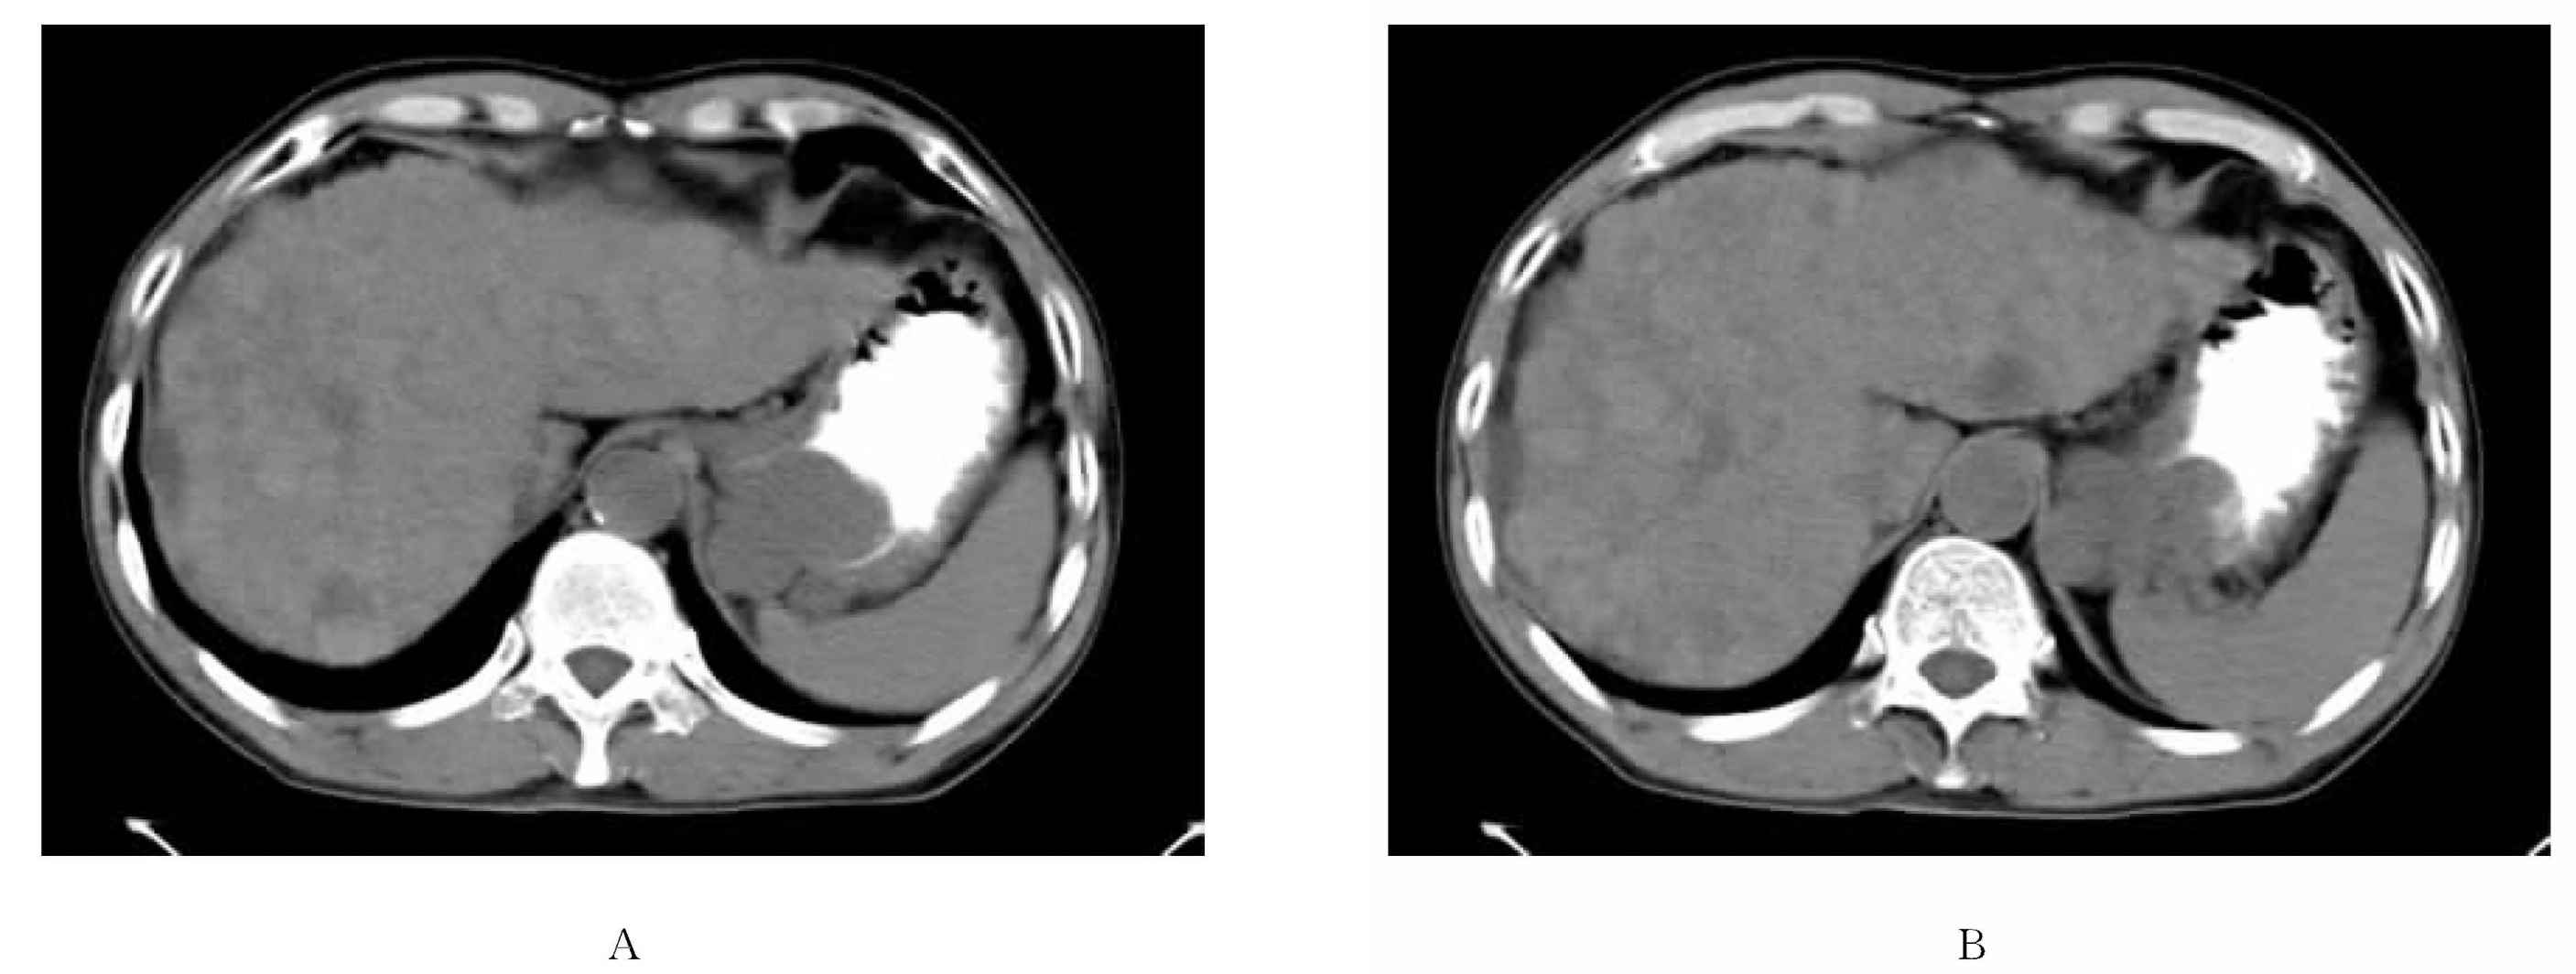
\includegraphics[width=.7\textwidth,height=\textheight,keepaspectratio]{./images/Image00287.jpg}
 \captionsetup{justification=centering}
 \caption{胃底静脉曲张\\{\small 胃底有分叶状软组织肿块(曲张的静脉),肝内有许多高密度硬化结节}}
 \label{fig11-15}
  \end{figure} 

\subsection{脂肪肝}

本病为肝脏酯类代谢功能异常,导致甘油三酯和脂肪酸等酯类物质过多沉积于肝实质内所致。正常肝内的脂肪含量低于5%,超过5%则可致脂肪肝。

\textbf{【病因病理】}
病因主要有:①肥胖症;②糖尿病;③囊性纤维变:约4%有脂肪肝;④酒精中毒;⑤肝代谢性疾病:如糖原沉积症及糖原合成酶缺乏症(部分患者存在脂肪肝)、脑病-脂肪肝综合征(Reye综合征);⑥营养不良类疾病;⑦肝炎、肝硬化;⑧药物所致:如应用糖皮质激素、化疗药物等;⑨库欣综合征患者和妊娠等。

病理镜下见肝细胞浆有大量脂肪堆积,使肝细胞胀大出现脂肪空泡。也可见肝细胞坏死、多核细胞浸润和胆汁潴留。肝脏可有不同程度肿大。

\textbf{【临床表现】} 肝大,血酯升高,还可有原发病之临床症状。

\textbf{【CT表现】}

1.弥漫型脂肪肝

诊断标准:一般参照脾的CT值,正常人肝的CT值总是高于脾脏。如果肝的CT值低于脾脏的CT值即可诊断为脂肪肝。也有文献认为,肝/脾CT值之比<0.85,则可诊断脂肪肝。

正常肝实质明显高于血管密度,肝静脉和门静脉主支清晰可辨。脂肪肝时,肝实质密度普遍下降并与血液密度接近时,两者的密度差异缩小或消失,肝内血管变得模糊不清或不能显示。严重脂肪肝时,肝密度呈负值,平扫血管呈相对高密度影,其表现如同增强的血管(图\ref{fig11-16}A)。

分度:CT平扫分为3度。①轻度:肝衰减值轻度低于脾,CT值约35~45Hu;②中度:肝衰减值明显低于脾,对比明显,肝内血管显示不清,CT值约25~35Hu;③重度:肝衰减值显著降低,且肝实质与肝内血管形成鲜明对比,CT值约-15~18Hu。

2.局灶型脂肪肝

又称为局限性脂肪肝。平扫多呈界限不明显的低密度区,如地图状(图\ref{fig11-16}B)。少数呈圆形或椭圆形、结节状低密度灶(好发于左叶内段镰状韧带旁和肝门旁),易误诊为肿瘤或其他病变。增强扫描病变范围和形态不变,CT值可轻度升高,但密度均匀一致。无占位效应,亦无门静脉及肝静脉等阻塞、移位表现有助于诊断和鉴别诊断。

总之,本型有以下4个特征:①通常为非球形病灶,界限不清,呈移行性;②无占位效应,增强扫描往往见血管进入病灶内,无周围血管受压推移表现;③增强扫描CT值升高不及正常肝组织及脾,形成更明显的密度差异;④其强化的时间-密度曲线与正常肝组织类似。

肝血管穿行于低密度的肝实质内,且无扭曲或狭窄虽是脂肪肝(弥漫型、局灶型)的较特征表现,但偶可见于淋巴瘤、转移性腺癌、转移性黑色素瘤等。

3.弥漫型脂肪肝残留的正常肝岛

残留的正常肝岛多发生于肝包膜下沿叶间裂或胆囊分布(图\ref{fig11-16}C、D)。这是由于体循环的包膜穿静脉或副胆囊静脉以及第3血供与门静脉的小分支直接沟通,局部门静脉的血流减少,动脉-门静脉短路,局部门静脉血流稀释,脂肪沉积减少,故仍保持正常肝密度。膈动脉和肋间动脉等对肝周局部的供血可能是肝岛好发于肝周边部的原因。

\begin{figure}[!htbp]
 \centering
 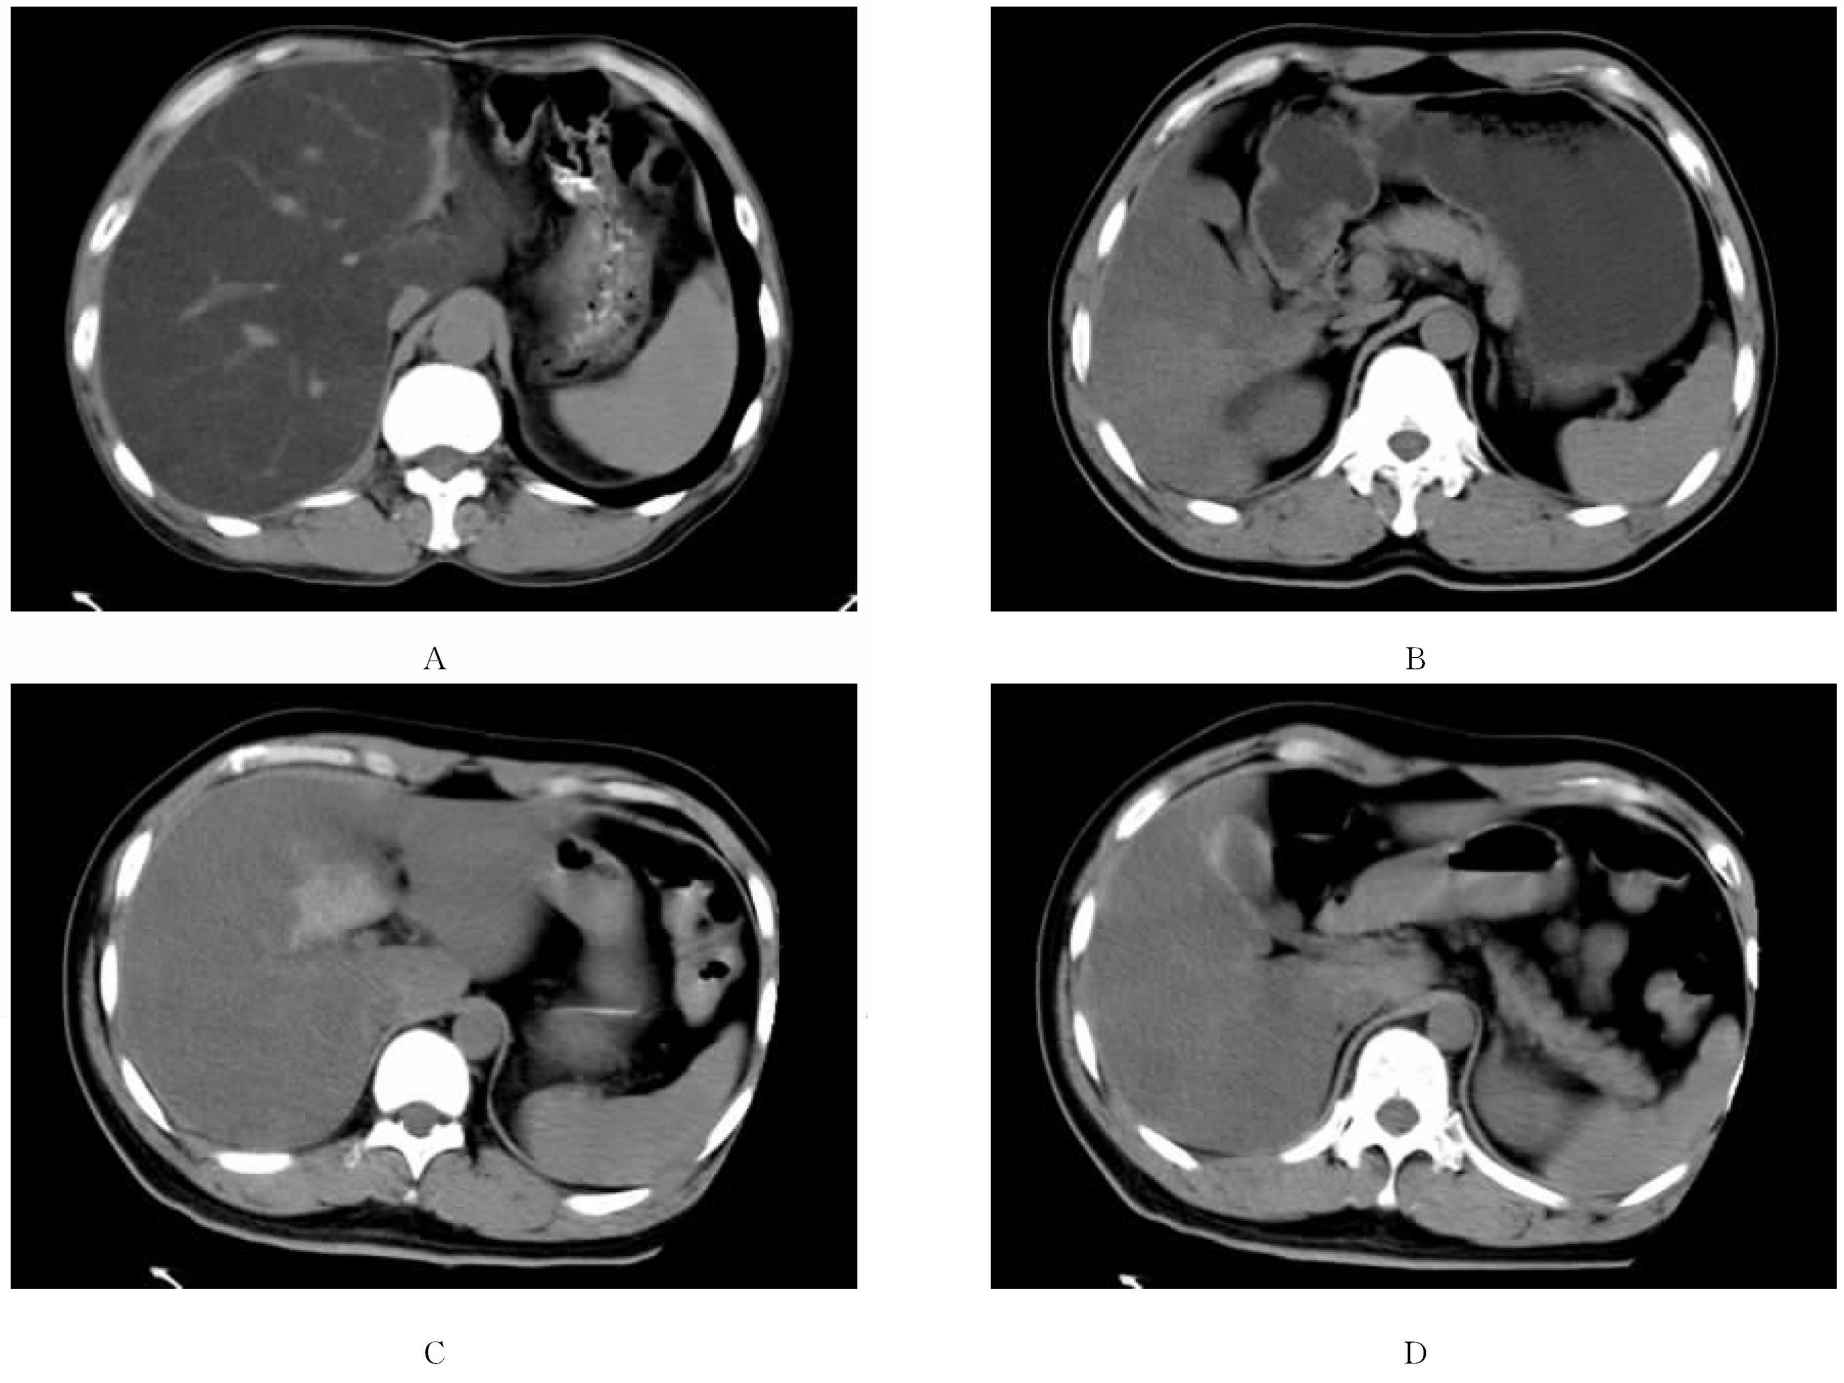
\includegraphics[width=.7\textwidth,height=\textheight,keepaspectratio]{./images/Image00288.jpg}
 \captionsetup{justification=centering}
 \caption{脂肪肝\\{\small A、B非同一患者。A为重度弥漫型,血管密度明显高于肝脏,如同强化的血管;B为局灶型,肝右叶前下段楔形低密度灶。C、D为同一患者,表现为沿叶间裂和胆囊分布的相对高密度区(正常肝岛)}}
 \label{fig11-16}
  \end{figure} 

其CT特点为:①肝岛呈相对高密度,其扁平的形状有助于与肿瘤鉴别;②肝岛与肝缘交角多为钝角,而肝边缘的肿瘤与肝缘的交角多为锐角;③肝岛边缘模糊,无占位效应;④增强扫描密度均匀。

4.弥漫型脂肪肝合并肿瘤

重度脂肪肝者,肿瘤呈相对高密度;中度脂肪肝者,肿瘤可呈高、等、低密度影;有报道平扫时肝内有全周或部分高密度环影是肝内占位病变的一个重要征象。增强扫描有助于肿瘤的检出和确诊。

\subsection{肝血红蛋白沉着症}

本病又称肝血色素沉着症、肝含铁血黄素沉着症、肝过量铁质沉积症、血色病。

\textbf{【病因病理】}
①先天性:为遗传性疾病。因肠黏膜细胞缺陷,导致铁的过量吸收及器官内的过量沉积,肝、脾、胰腺、肾、肾上腺、心肌、淋巴结等易受累。多合并肝硬化、糖尿病及心肌病等,还常见皮肤色素沉着及性腺萎缩。②后天性:多因各种原因之顽固性贫血,而长期反复大量接受输血,过剩的铁质沉着于肝、脾、骨髓等网状内皮系统,而不伴脏器实质损害。其他脏器多不受累或受累较轻。

\textbf{【临床表现】}
先天性者可有肝硬化、皮肤色素沉着、糖尿病、心肌病和性腺萎缩等一系列临床表现。后天性有顽固性贫血且大量输血病史。晚期可发生肝硬化,5.8%~42.9%继发肝癌。

\textbf{【CT表现】}
平扫肝密度普遍性增高,CT值约为75~132Hu,且病情与CT值升高呈正比关系;门静脉及肝静脉则相对呈极低密度改变。本病还可伴有脂肪肝,而致肝实质密度并不升高,故肝密度正常并不能完全排除肝血色素沉着症。由于铁是顺磁性物质,MR检查明显缩短T\textsubscript{2}
有助于确诊。

先天性者还可表现胰腺、肾、肾上腺密度增高;继发性者,除肝脾密度增高外,而无胰腺受累。

\subsection{肝糖原沉积病}

本病是一种先天性糖原代谢紊乱性疾病。

\textbf{【病因病理】}
多数由于糖原代谢酶的缺陷而导致糖原分解或合成障碍,从而产生不同组织器官中糖原或异形糖原的过多蓄积。主要受累的脏器有肝、肾、肌肉和小肠等。本病根据缺陷的酶不同而分为6型,其中Ⅰ、Ⅲ、Ⅳ型主要影响肝脏。

\textbf{【临床表现】}
本病以Ⅰ型最常见,为肝内葡萄糖-6-磷酸酯酶缺乏所致。典型的表现为新生儿期出现肝大、低血糖、心肾增大、高乳酸血症、脂肪代谢紊乱和血尿酸增多等。

\textbf{【CT表现】}
①肝显著增大。②肝密度的改变:当肝细胞内糖原聚集到一定量时肝密度增高。但本病常并发不同程度的弥漫性脂肪肝,而致肝密度升高、正常或降低。脂肪浸润好发于较大儿童。

此外,本病可继发肝硬化、门静脉高压、腺瘤甚至肝癌而出现相应表现;X线平片还可见骨骼成熟延迟、骨密度下降以及尿酸石、痛风改变,而有助于诊断。

\subsection{肝豆状核变性}

本病是一种常染色体隐性遗传病,表现为铜代谢障碍。

\textbf{【病理】}
主要病理改变为神经系统的豆状核变性和肝脏出现坏死后肝硬化。

\textbf{【临床表现】}
多见于10~25岁。典型表现为进行性加剧的肢体震颤、肌张力增高,以及眼角膜缘与巩膜交界处出现绿褐色色素环即Kayser-Fleioker环,为本病的特征性表现。

\textbf{【CT表现】}
①本病肝的铜蓄积较轻微,故肝的密度并无显著增加,而肝硬化的表现反而明显;②颅脑表现为以豆状核为主的对称性低密度改变。

此外,本病可继发骨质疏松,椎体、骨盆等CT示骨盐定量降低,小关节边缘毛糙和软骨下骨质吸收及小片碎骨,韧带、肌腱的过早钙化或骨化等也有助于诊断。

\subsection{肝淀粉样变性}

淀粉样变性为代谢性疾病,淀粉样物质沉积于细胞外,主要沿血管壁分布,可侵及肝、脾、胰、胃肠道、心肌和肾脏等。临床无特异性。

\textbf{【CT表现】}
肝增大,可见弥漫性或局限性低密度区,增强不明显,肝内血管不移位。脾脏亦有类似表现。总之,本病与脂肪肝表现相似,但脂肪肝无脾脏异常改变。

\subsection{布加(Budd-Chiarl)综合征}

本病是因肝静脉和(或)肝静脉开口水平上下的下腔静脉阻塞或狭窄,导致窦后性门静脉高压的一组临床综合征。最早由Chiarl(1899年)和Budd(1945年)分别报告。

\textbf{【病因】}
主要有3类:①肝静脉血栓形成:欧美国家多见;②肿瘤压迫肝静脉或下腔静脉;③下腔静脉肝段阻塞:多为先天性,亚洲国家多见。总之,本病可见于先天性异常和血液凝固性过高、妊娠、口服避孕药、肿瘤、外伤等。虽然本征可由肝癌所致,但肝癌亦可由慢性布加综合征发展而来。

\textbf{【临床表现】}
病程较长,同时存在下腔静脉阻塞和继发性门静脉高压的临床表现。前者如下肢肿胀、静脉曲张、小腿及踝部色素沉着以及腹壁静脉曲张(侧支通道);后者如腹胀、肝脾大、腹水、黄疸和食管静脉曲张等。

\textbf{【CT表现】}

\subsubsection{急性期}

1.平扫:肝弥漫性增大,肝实质呈弥漫性低密度,反映肝实质严重充血。

2.增强扫描:①下腔静脉和大的肝静脉分支内血栓呈管腔内低密度,管腔周围有一个强化的边,可能是其滋养血管显影所致;②增强扫描肝实质呈中心性斑片状低密度,肝周边部无明显强化,说明存在离肝的门静脉血流;③肝实质内的出血和坏死呈无强化的低密度区。

\subsubsection{慢性期}

1.平扫:常表现为腹水、肝脾增大和肝硬化。可见周边部非节段性萎缩或肝萎缩,而尾状叶正常或增生肥大。周边部的低密度区反映了肝实质充血或出血性坏死,或静脉阻塞所致的纤维化。

2.增强扫描:①下腔静脉和肝静脉内血栓,表现为管腔扩大和腔内充盈缺损;②肝静脉可不显示(图\ref{fig11-17});门静脉分支可变细、僵直;还可见肝动脉增粗并肝内分支增多;③肝中央区呈放射状进行性斑片状强化,从大的门静脉分支向周边部呈放射状扩展,提示此区域有正常的门静脉向肝供血;④肝周边部先呈低密度,以后渐进性迟发均匀强化,数分钟后整个肝呈等密度,说明该部有正常或相对的增强的动脉血流而窦后压力增高,门静脉血流逆向;⑤可见肝内、肝外侧支循环血管影,其中肝内者位于肝包膜下和外周带,呈网格状连接于肝静脉及其与副肝静脉之间。

\begin{figure}[!htbp]
 \centering
 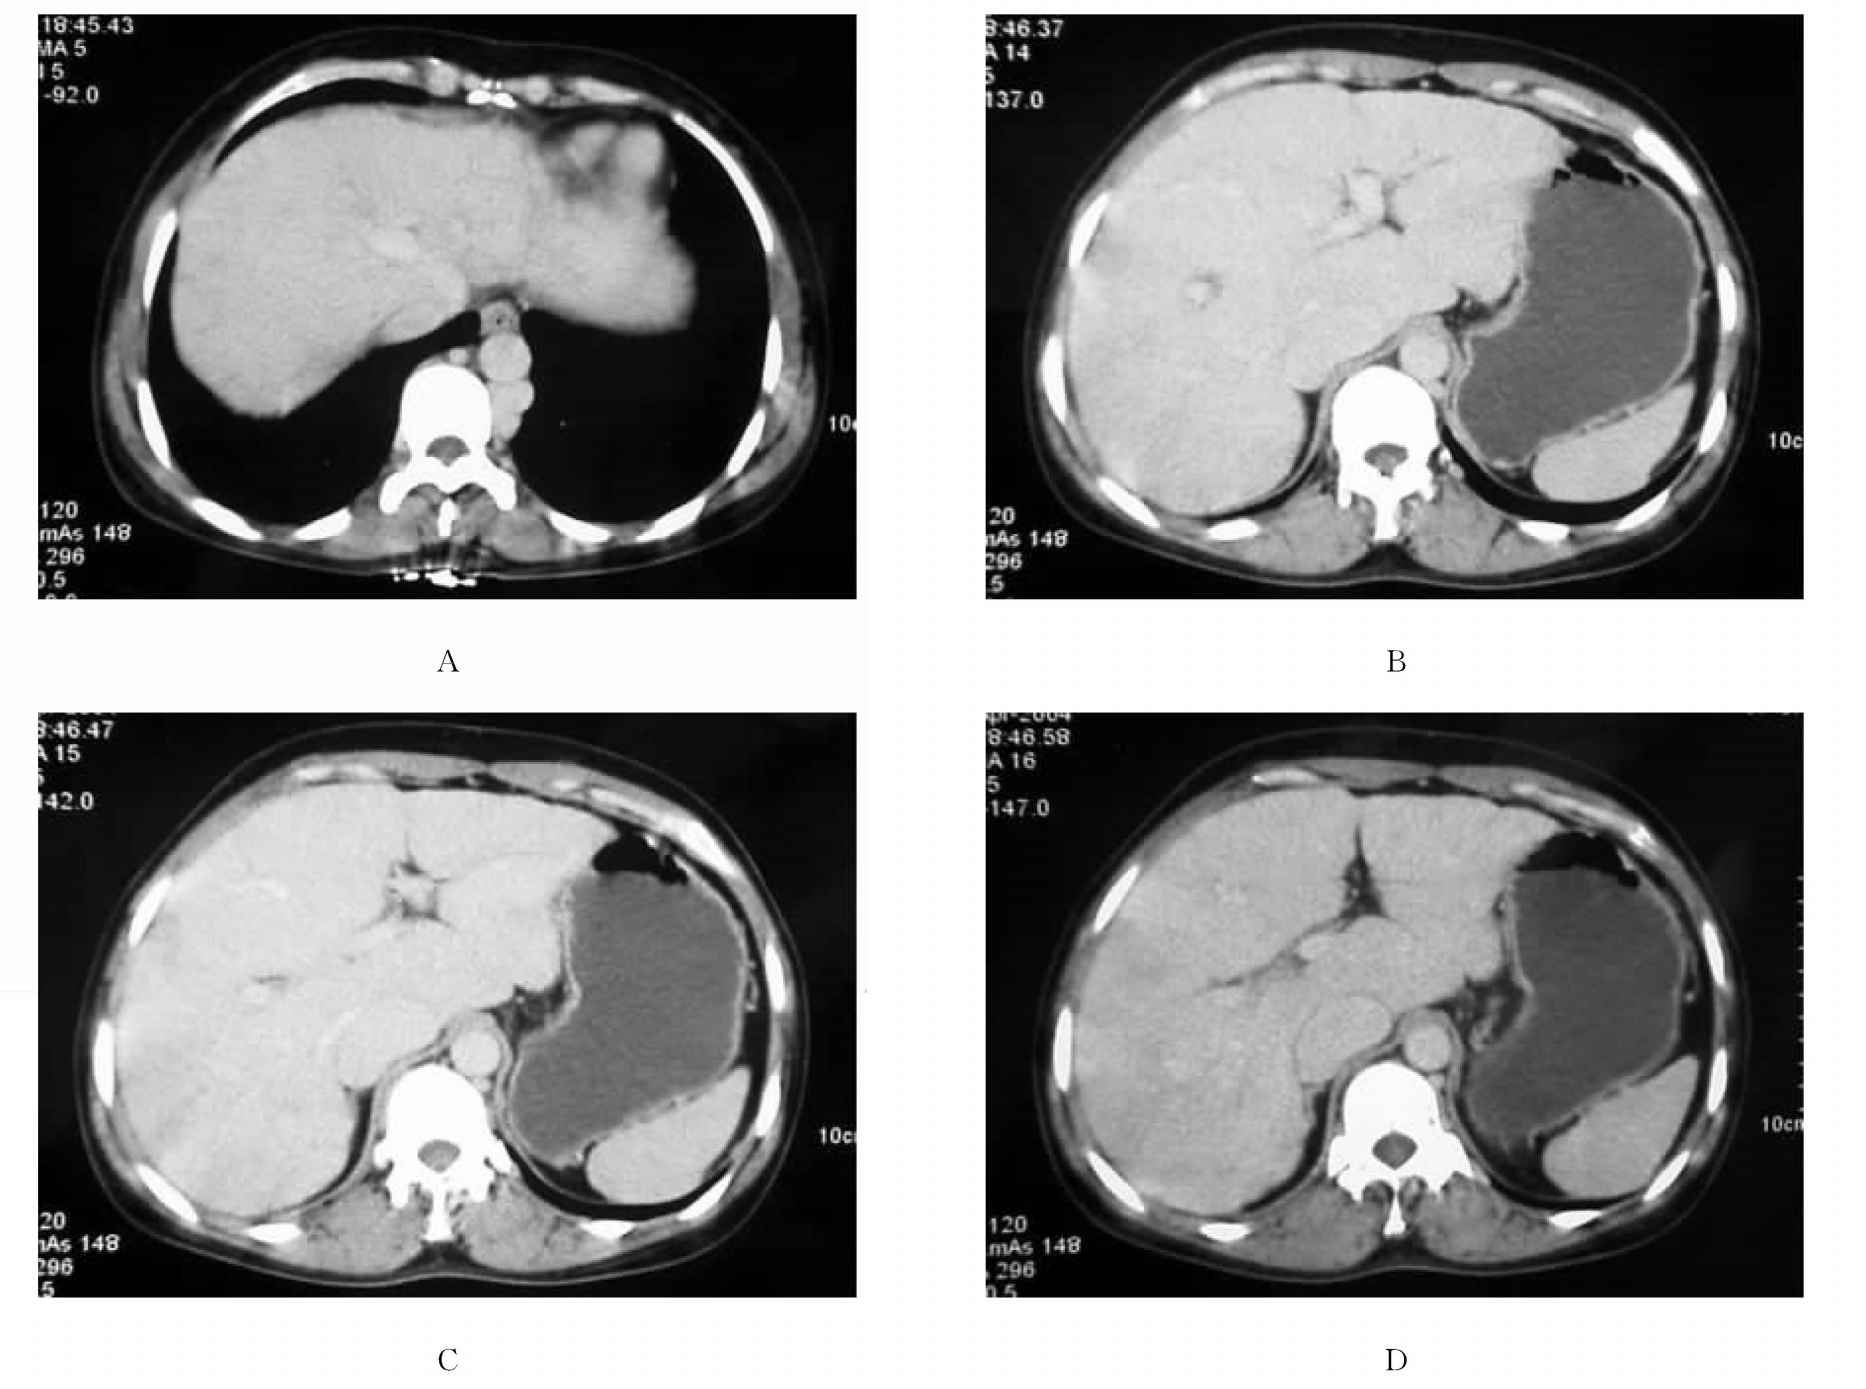
\includegraphics[width=.7\textwidth,height=\textheight,keepaspectratio]{./images/Image00289.jpg}
 \captionsetup{justification=centering}
 \caption{布加综合征\\{\small A~D为同一患者增强扫描表现,肝静脉未明确显影;肝脏增大,以尾状叶为著}}
 \label{fig11-17}
  \end{figure} 

总之,肝淤血引起的门静脉血流受阻是肝实质异常强化的基础,门静脉血流量减少是引起肝脏强化程度减低和延迟强化的主要原因。

3.再生结节:慢性期肝内可有再生结节形成,只有部分能显示,增强扫描所显示的结节多于平扫。①平扫大部分结节呈等密度或因较小而不易显示,所显示者多为高密度(与结节周围肝实质的淤血、坏死造成的低密度有关)。②增强扫描动脉期多明显均一强化而呈高密度(富血供),门脉期仍呈稍高密度。有时结节周围有强化不明显的低密度环,低密度环与结节周围的组织萎缩、淤血及肝窦扩张有关。

\subsection{门静脉血栓形成}

\textbf{【病因病理】}
常见的原因有肿瘤、感染、胰腺炎、肝硬化门静脉高压、外伤、血液高凝状态或肝静脉阻塞等。病变范围可局限在门静脉主干或大的分支,以及脾静脉、肠系膜上静脉,或广泛累及整个门脉系统。门脉血栓形成又将导致门脉高压和大量侧支血管形成。

\textbf{【临床表现】} 常存在急性或亚急性腹部疼痛,偶有脾肿大。

\textbf{【CT表现】}
急性期门静脉轻度扩张,平扫除新鲜血栓呈高密度外,一般与血液密度一致;增强扫描可见血栓形成段门静脉腔无强化,管壁增厚,而扩张的滋养血管显著强化;部分呈腔内充盈缺损表现。慢性期可显示血管再通、扩张的侧支循环等,还可见门脉海绵样变表现。

\subsection{肝梗塞}

因肝脏为双重供血,肝动脉阻塞引起肝梗塞少见。

\textbf{【病因】}
肝动脉阻塞的原因有动脉粥样硬化、栓塞、血栓形成、血管炎或低血压及休克,偶见于妊娠或口服避孕药后。

\textbf{【CT表现】}
与脾、肾梗塞类同。①增强后呈周围性楔形低密度影;偶尔可涉及整个肝叶,导致弥漫性低密度;亦可位于中央呈圆形。②吸收时最初表现为梗塞区边缘模糊,继而变为散在边缘锐利的低密度灶。③继发坏死可导致气体积聚于梗塞中央,并可感染。④慢性征象包括受累肝叶、肝段的萎缩,并伴有残留的低密度和囊变。

\subsection{被动性肝充血}

\textbf{【病因病理】}
被动性肝充血是充血性心力衰竭或缩窄性心包炎者的一种临床和病理表现,中心静脉压升高反向传导至肝静脉系统,引起中央小叶充血,最终导致肝大和肝功能不全。

\textbf{【临床表现】}
患者常有肝大和肝区触痛。并有心衰或缩窄性心包炎等病史。

\textbf{【CT表现】}
①肝增大。增强扫描早期可见肝实质呈斑片状不均匀强化;延迟扫描呈等密度;部分病例可见门脉周围低密度水肿。②下腔静脉和肝静脉扩张,动态增强扫描早期在肝实质强化前肝静脉逆向显影。

\subsection{肝紫癜病}

本病最早报道于1986年,是在肝内分布着许多或无数血斑的一种病变,不是血管瘤。

\textbf{【病因病理】}
血斑大小1~5mm,可分为两型。①实质型:血斑分布在肝实质内,形态不规则;镜下见小血腔无内皮细胞被覆,腔内除血液外,还可见坏死肝组织的碎屑,血腔与中央静脉不相通。此型病因尚不明,有报道由于使用乙基去甲基睾丸酮治疗其他疾病而引起的,且死于肝功能衰竭。②静脉扩张型:血斑呈圆形,位于小叶中央;血腔壁有内皮细胞被覆。邻近肝索有被压迫性改变。此型病因也不明,似与血管壁的病变有关。

\textbf{【临床表现】}
多见于成人,临床无任何明显症状。但以上两型往往发现合并重型结核病或其他消耗性疾病。严重者可致肝功能衰竭;破裂出血可导致失血性休克甚至死亡。穿刺活检无法获得有价值的病理细胞或组织,且有大出血的危险。

\textbf{【CT表现】}
关于其CT诊断价值尚有争议。平扫缺乏特征性,多表现为低密度影,脂肪肝时反而呈高密度。增强扫描可见病灶不规则形强化或边缘性强化。这种强化表现实际是血液滞留腔和血窦的直接交通,导致对比剂进入而显影。国外有学者发现增强扫描的强化特点是从病变的中心向边缘逐渐扩展。有些病灶不强化是被机化的血栓阻塞所致。

本病应注意与囊肿等其他囊样病变相鉴别。

\protect\hypertarget{text00019.html}{}{}

